%
% Author: Marzia Corvaglia
%         DEA - University of Brescia IT
%
% Dte:  21 oct. 2005
%

\documentclass[11pt,oneside]{book}
\usepackage[dvips,colorlinks=true]{hyperref}
\hypersetup{
	bookmarksnumbered=true,
	linkcolor=black,
	citecolor=black,
	pagecolor=black,
	urlcolor=black,
}

\usepackage[latin1]{inputenc}
\usepackage[italian]{babel}

\usepackage[T1]{fontenc}
\usepackage{setspace}
\usepackage{graphicx}
\usepackage{amsmath,amsfonts,amssymb}
\usepackage{makeidx}
\usepackage{wrapfig}
\usepackage{footnote}
\usepackage{subfig} 
\usepackage{tabularx}
\usepackage{longtable}
\usepackage{booktabs}
%\usepackage{psfrag}
\usepackage{hyperref}
\usepackage[usenames]{color}
\usepackage[table]{xcolor}
%\usepackage{ctable}
\usepackage{threeparttable}
\definecolor{comm}{rgb}{0.27,0.31,0.21}

\usepackage{listings}
\lstset{language=PHP,
basicstyle=\scriptsize,commentstyle=\tiny,
keywordstyle=\color{black}\bfseries,
commentstyle=\color{comm},
stringstyle=\color{black},
showstringspaces=false,
numbers=left,
numberstyle=\tiny}
\addto\captionsitalian{\renewcommand{\lstlistingname}{Codice}}
%-------------------------------
%          geometry
%-------------------------------

\usepackage[width=0.75\paperwidth,height=0.8\paperheight]{geometry}

%-------------------------------
%         fancy header
%-------------------------------

\usepackage{fancyhdr}
\pagestyle{fancy}

\renewcommand{\chaptermark}[1]{\markboth{\thechapter .\ #1}{}}
\renewcommand{\sectionmark}[1]{\markright{\thesection .\ \it #1}}
\fancyhf{}

\fancyhead[LE,RO]{\thepage} \fancyhead[LO]{\rightmark}
\fancyhead[RE]{\rm\leftmark}

\fancypagestyle{plain}{ \fancyhead{}
\renewcommand{\headrulewidth}{0pt}
\fancyfoot[C]{\thepage} }
\linespread{1.3}
%formattazione del codice sorgente
%\lstset{basicstyle=\scriptsize,commentstyle=\tiny,
	%stringstyle=\ttfamily, numberstyle=\tiny, stepnumber=2, numbersep=10pt,
	%morecomment=[s]{//},
	%morecomment=[s]{/*}{*/}
%}
%\lstloadlanguages{ C++ }
%-------------------------------
%         document
%-------------------------------
\makesavenoteenv{tabular}

\hyphenation{per-mes-so a-na-liz-za-re si-mu-la-zio-ne ge-stio-ne o-pe-ra-zio-ni ra-pi-di-t� se-gno u-ti-liz-zo im-me-dia-ta-men-te que-sta uten-te fun-zio-na-li-t� com-pa-ti-bi-li-t� dis-po-si-zio-ne ne-ces-sa-ria in-ge-gne-ri-a ne-ces-sa-rio auto-rizzati ra-pi-da disposi-zione a-spet-ti mo-di-fi-ca dif-fe-ren-ti} 

\begin{document}

\pagenumbering{roman}

% frontespizio

\begin{titlepage}

 \begin{center}
    \scshape   Universit� degli Studi di Brescia\\
    \scshape  Facolt� di Ingegneria\\
    \scshape Corso di Laurea Specialistica Informatica\\
    \vspace{1cm}
    \begin{figure}[!ht]
     \begin{center}
      
\includegraphics[width=5cm]{stemma.eps}
     \end{center}
    \end{figure}
    \vspace{1cm}
    \bfseries \Large VALUTAZIONE DI USABILIT\'A \\ DEL SITO WEB DELLA DELL Inc.\\


    \vspace{4cm}
    \upshape \mdseries \normalsize

  \begin{tabular}{p{6cm}@{}p{11cm}}
		Studente:\\
      \bf{Lombardi Luca} & matricola \bf{75814}  \\
		\bf{Rizzardi Enrico} & matricola \bf{59673}   \\
	\end{tabular}
 	\begin{tabular}{p{17cm}}
     	Docente:\\
      \bf{Prof.ssa Daniela Fogli} \\
	\end{tabular}



    \vspace{1cm}

    \vfill \it \large
    Anno Accademico 2008-2009
 \end{center}

\end{titlepage}


\tableofcontents

% ----- capitoli  -----

\cleardoublepage
\pagenumbering{arabic}
\cleardoublepage
\chapter{Introduzione}
Il sito web www.dell.it non � altro che la trasposizione italiana del sito internet www.dell.com, portale informatico dell'omonima casa produttrice di personal computer. Tale sistema si propone, sia come vetrina/negozio per soluzioni notebook e desktop, per accessori per pc, materiale elettronico di varia natura, come ad esempio televisori, sistemi home theater, sia come portale per accedere al supporto per i prodotti sopra citati venduti dall'azienda. Le soluzioni offerte dalla Dell Inc. riguardano sia i clienti privati con un ``Business to Consumer'' che i clienti aziendali offrendo un ``Business to Business''.\\
Quello che si propone la Dell Inc. con questo sito web, � di avere un contatto diretto con i propri clienti, eliminando le grandi catene di distribuzione e intermediari. Tale soluzione le consente di avere prezzi pi� concorrenziali, offrire la possibilit� di ``personalizzare'' molti prodotti e di garantire servizi post-vendita che fidelizzino il cliente alla societ� texana.\\
Per garantire questo tipo di commercio la Dell Inc, ha puntato molto sull' e-business, categoria nella quale possiamo collocare il sito web preso in esame. Il commercio elettronico, come una qualsiasi altra transazione economica si fonda su diverse fasi:
\begin{itemize}
\item La transazione economica si compone di una fase di ricerca, in cui il cliente cerca sul mercato i fornitori potenzialmente in grado di soddisfare i suoi requisiti
\item {\it Negoziazione}: il cliente interagisce con i fornitori individuati per vericare se e a quali condizioni possono essere soddisfatti i propri requisiti. Questa fase si conclude con la scelta del fornitore e del prodotto
\item {\it Esecuzione}: il bene scelto in precedenza viene consegnato al cliente
\item Controllo, ha l'obiettivo di gestire eventuali eccezioni che possono vericarsi (per esempio, la fornitura al cliente di un bene difettoso).
\end{itemize}
Nel caso della Dell Inc. tutte queste fasi sono state automatizzate e informatizzate, pertanto il possedere uno strumento informatico facile da gestire e funzionale per i clienti diventa di fondamentale importanza per il business dell'azienda. Lo scopo di tale relazione � verificare l'usabilit� della versione italiana di tale portale web.\\
Nel primo capitolo presenteremo il sito web in questione e successivamente  forniremo la pianificazione dell'attivit� svolta e definiremo il profilo utente.

\section{Descrizione del sistema}
Il portale preso in esame, {\it www.dell.it}, appartiene alla categoria dei Web System Information del tipo e-commerce e informativo: consente di scegliere e acquistare una vasta gamma di prodotti high tech, mentre dal punto di vista informativo si possono apprendere svariate notizie riguardanti l'azienda, dalla storia della Dell Inc., alle politiche ambientali adottate dal'azienda.\\
\begin{figure}[!h]
\centering
\includegraphics[scale=0.75]{figure/home_page.eps}
\caption{Home page del sito web www.dell.it} \label{fig:home_page}
\end{figure}\\
L'home page, come mostrata in figura\ref{fig:home_page}, pu� essere suddivisa in tre macroaree e in una intestazione a pi� pagina. Scorrendo la pagina dall'alto verso il fondo troviamo:
\begin{enumerate}
\item Un primo men� orizzontale che consente di accedere rapidamente alle pagine informative suddivise per clientela (privati, piccole-medie imprese, pubblica amministrazione, grandi imprese) e a fianco un piccolo men� per richiedere assistenza o effettuare il login. Sulla sinistra � sempre presente il logo dell'azienda che, oltre allo scopo pubblicitario, ha anche la funzione di rimandare l'utente alla home page.
\item Nella parte centrale � stato riservato un ampio spazio alla vetrina dei prodotti maggiormente pubblicizzati, offerte speciali. Sono perlopi� immagini a ciclo continuo che occupano l'intera area. Anche tali immagini sono dei link che rimandano al prodotto visualizzato in quel momento.
\item A fondo pagina troviamo un secondo men� orizzontale che riporta ulteriori link alle aree descritte al punto 1. Troviamo inoltre anche aree dedicate all'account personale dell'utente, al supporto e alle informazioni sulla societ�.
\end{enumerate}
Come � chiaramente visibile, il portale web � assai esteso sia in ampiezza, con un buon numero di sezioni, sia in profondit�, con un ampio numero di livelli e sotto livelli che appartengono ad ogni sezione; pertanto si � stabilito di concentrare e limitare la valutazione alla sezione a noi pi� affine, ossia alla sezione {\it PER LA CASA}, denominazione che � stata data per la categoria degli utenti privati, ossia persone che non hanno la possibilit� di scaricare l'IVA, e hanno richieste assai differenti dalle aziende: ad esempio il fattore di personalizzazione per i privati � molto elevato (si va dall'aspetto estetico fino ai componenti dell'intero computer) ed � presente su molteplici modelli; per i clienti aziendali questo aspetto � molto limitato se non addirittura assente.\\
La figura \ref{fig:home_privati1} mostra la pagina con la quale un utente privato si trover� a interagire fin dall'inizio, e con la quale potr� iniziare la navigazione per ottenere ci� che desidera, sia che sia un un ``acquisto'' o che sia del ``supporto''. Di default il sistema mostra la sezione ``acquisti''. Presenteremo queste due parti oltre alla home page, poich� sono le due pagine web con le quali l'utente dovr� interagire maggiormente, pertanto sono di fondamentale importanza per una buona navigabilit� e usabilit�.\\
Analizzando nel dettaglio la pagina caricata di deafult, troviamo che � divisa anch'essa in tre parti: l'intestazione composta da una serie di titoli che consentono di accedere a tutte le varie categorie di prodotti offerti. Ogni categoria (offerti speciali, Notebook \& Mini, etc...) apre un men� a discesa che consente di scegliere una determinata categoria di modelli. 
\begin{figure}[!h]
\centering
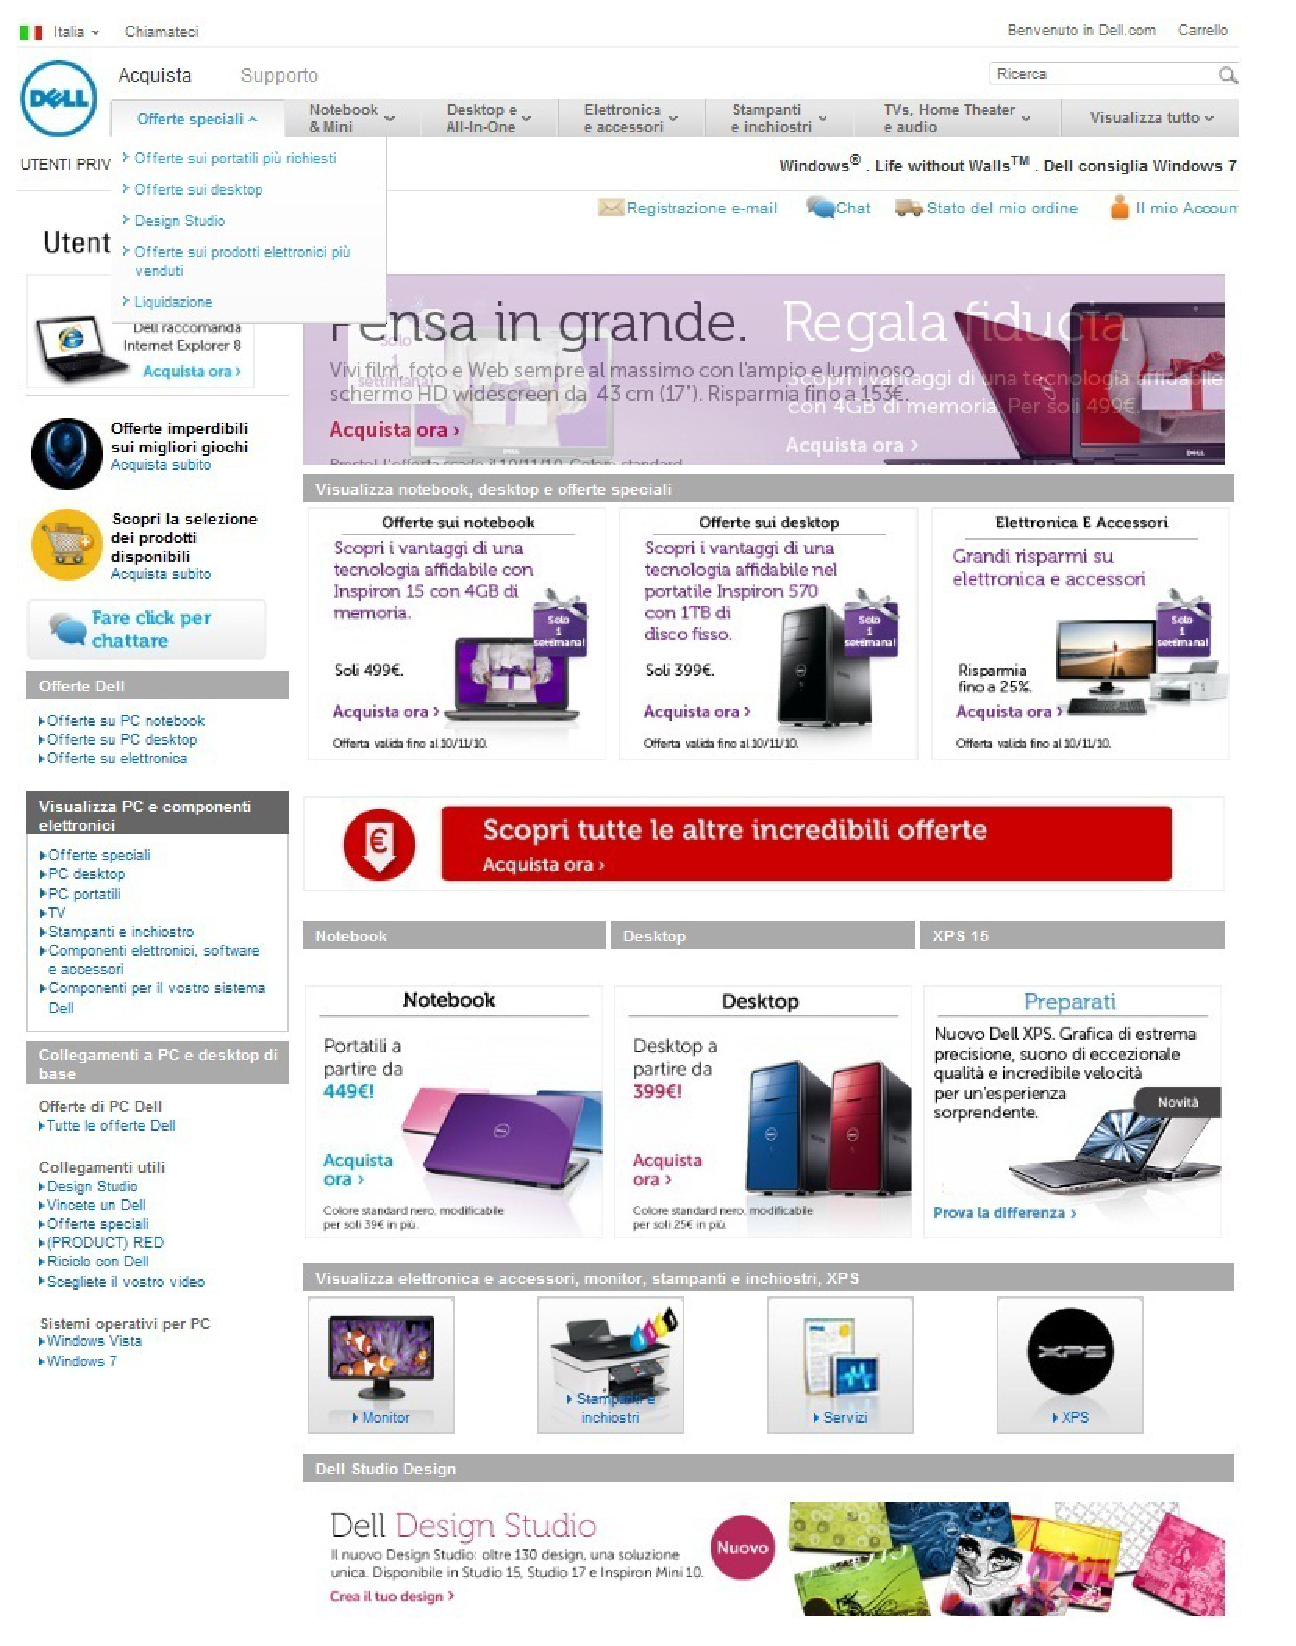
\includegraphics[scale=0.73]{figure/privati1.eps}
\caption{Home page sezione ``Per la casa''. Si pu� notare il men� a discesa della sezione ``Offerte speciali''} \label{fig:home_privati1}
\end{figure}\\
\newpage
Le sezioni raggiungibili da tramite questo men� sono:
\begin{itemize}
\item {\bf Offerte speciali}: racchiude una serie di link diretti che conducono alle offerte sulle varie categorie di prodotti. Tali offerte possono essere relative a prodotti che oramai la Dell non ha pi� intenzione di produrre oppure prodotti maggiormente venduti che sono associati a un qualche genere di promozione.
\item {\bf Notebook \& Mini}: racchiude tutte le categorie di notebook e pc mini che la Dell Inc. produce. Troviamo in testa due collegamenti alle offerte e ai prodotti in liquidazione a cui succedono vari link che visualizzano i diversi prodotti: prima il nome della famiglia in azzurro chiaro e appena sotto in grigio tutti i modelli che appartengono a tale famiglia; vengono mostrati all'utente in ordine crescente di prestazioni, mentre a fondo men�, separato da una linea troviamo link d'utilit� come il confronto tra prodotti diversi.
\item {\bf Desktop e All-in-One}: Come per la famiglia dei portatili lo schema di visualizzazione rimane lo stesso: il collegamento alle offerte e liquidazione, successivamente le varie soluzioni desktop e All-in-One, con la suddivisione famiglia-modello, sempre mostrate in ordine crescente di prestazioni e in fondo al men� i link d'utilit� per il confronto e l'accesso diretto agli accessori
\item {\bf Elettronica e accessori}: tale men� permette di accedere a un insieme di prodotti molto eterogeneo: dai lettori mp3 agli accessori per notebook e desktop. In tale men� la visualizzazione non prevede che per ogni categoria vengano elencati anche tutti i nomi dei prodotti, ma solamente la categoria a cui appartengono (Mp3, GPS, etc...)
\item {\bf Stampanti e inchiostri}: racchiude tutte le stampanti che possono essere acquistate tramite il sito internet. Lo schema di visualizzazione � lo stesso usato per la sezione ``Elettronica e accessori'': vengono mostrate solamente le varie famiglie di prodotti senza elencare i singoli modelli
\item {\bf TVs, Home Theater e audio}: permette di accedere alle pagine in cui vengono mostrati le soluzione per l'intrattenimento domestico, con tv di varia grandezza, soluzioni audio e video. Lo schema di visualizzazione � lo stesso degli ultimi due men�
\item {\bf Visualizza tutto}: apre un men� in cui compaiono tutti le categorie di prodotti precedentemente citati: un'intestazione in azzurro chiaro per la categoria (stessa dicitura precedentemente) e in grigio le varie famiglie che appartengono a tale categoria
\end{itemize}
Tornando ad esplorare la pagina (fig:\ref{fig:home_privati1}) troviamo una colonna posta sulla sinistra composta da una serie di link a pagine appartenenti alle sezioni alle quali si pu� accedere anche dai men� precedentemente citati; questo elenco riporta per la maggior parte link di maggior interesse, sono prevalentamente le pagine pi� richieste dall'utente. La restante parte della pagina � dedicata a una serie d'immagini, tutte con funzione di link, che riportano pubblicit� di offerte, nuovi prodotti, o comunque soluzioni che l'azienda vuole mettere in maggior risalto. A fondo della schermata troviamo un secondo men� riassuntivo comprendente tutta una serie di collegamenti che consentono all'utente di accedere alle sezioni prima elencate e in aggiunta anche alle sezioni riguardanti l'azienda, informazioni personali e condizioni d'uso. In ultimo vi � un trafiletto sulle offerte e condizioni generali sull'utilizzo del sito web (fig:\ref{fig:home_privati2}).
Come la maggior parte dei siti web di e-commerce fanno uso della metafora {\it carrello} per indicare tutti quei prodotti scelti dall'utente, configurati e pronti per essere acquistati, ma non ancora confermati definitivamente;nel nostro caso � presente un link diretto a tale elenco ed � sempre posto, in tutte le pagine della sezione ``acquisti'', in alto a destra.
\begin{figure}[!h]
\centering
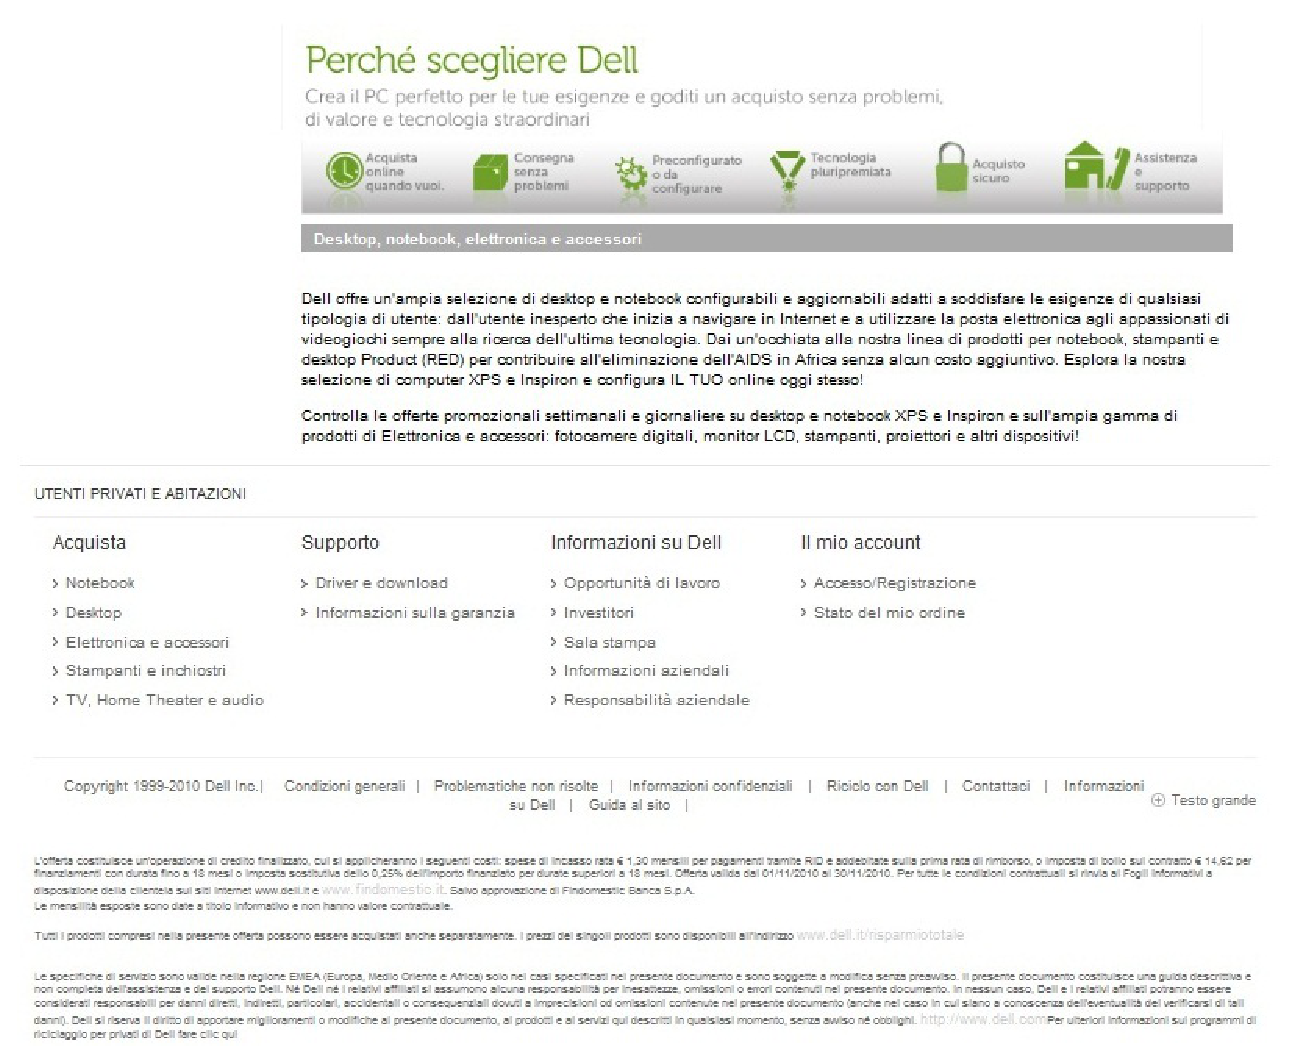
\includegraphics[scale=0.75]{figure/privati2.eps}
\caption{Fondo pagina della sezione ``Per la casa'' sezione ``Acquisti''} \label{fig:home_privati2}
\end{figure}\\
\newpage
Il passaggio alla sezione supporto � reso possibile dal posto in alto a sinistra con la scritta ``Supporto''. Nella pagina visualizzata troviamo che lo schema di  � lo stesso di quello usato per la sezione ``acquisti'': una barra orizzontale che mostra diverse utilit� di carattere generico (campo di ricerca,link al login,un link diretto alla home page, etc...), e in aggiunta un men� orizzontale che consente di accedere alle vere e propri categorie di supporto. Tali sezioni sono:
\begin{itemize}
\item {\bf Driver e download}: consente di scaricare varie tipologie di driver per accessori e prodotti Dell. Fornisce inoltre aiuto nel caso l'utente abbia problematiche a installare un sistema operativo differente su un prodotto Dell.
\item {\bf Assistenza per il prodotto}: fornisce manuali d'uso, risoluzione delle problematiche pi� comuni, aggiornamenti e supporto per il ritiro dei prodotti
\item {\bf Supporto per argomento}: le problematiche sono trattate per argomento; � da sottolineare che tali argomenti sono in massima parte argomenti di tipo software, specialmente sui vari sistemi operativi forniti all'acquisto di un computer, pertanto si trovano esclusivamente sistemi operativi Microsoft. Possiamo trovare anche aiuti sulla configurazione delle reti wireless o sulla sicurezza
\item {\bf Assistenza per l'ordine}: viene trattato tutto ci� che riguarda l'ordine di un utente: lo stato di avanzamento, la restituzione del prodotto, le segnalazioni di danneggiamento o di malfunzionamenti dello stesso
\item {\bf Informazioni sulla garanzia}: vengono date note informative sui termini legali della garanzia e delle varie estensioni proposte dalla Dell Inc. e accedere a particolari tipi di assistenza
\item {\bf Visualizza tutto}: come nel caso della precendente (sezione ``acquisti'') anche in questo caso tale dicitura consente di visualizzare un sommario di tutte le voce appena descritte, suddividendole in categorie come nel men� ed elenco le sottovoci del men� a discesa
\end{itemize}
Tornando ad analizzare la pagina nel suo complesso possiamo ritrovare a sinistra un elenco di link che riprendono ci� che possiamo trovare nel men� precedentemente descritto, suddivisi nelle medesime sezioni, mentre nella sezione centrale della pagina un ricco assortimento di icone e ulteriori link alle varie sezioni di supporto all'utente. Da tali icone si pu� accedere alle aree dedicate alla community e ai contatti diretti con gli operatori. 
A fondo pagina � riportato il medesimo schema della sezione acquisti con un elenco di tutte le categorie e delle condizioni generali d'utilizzo del portale.
\begin{figure}[!h]
\centering
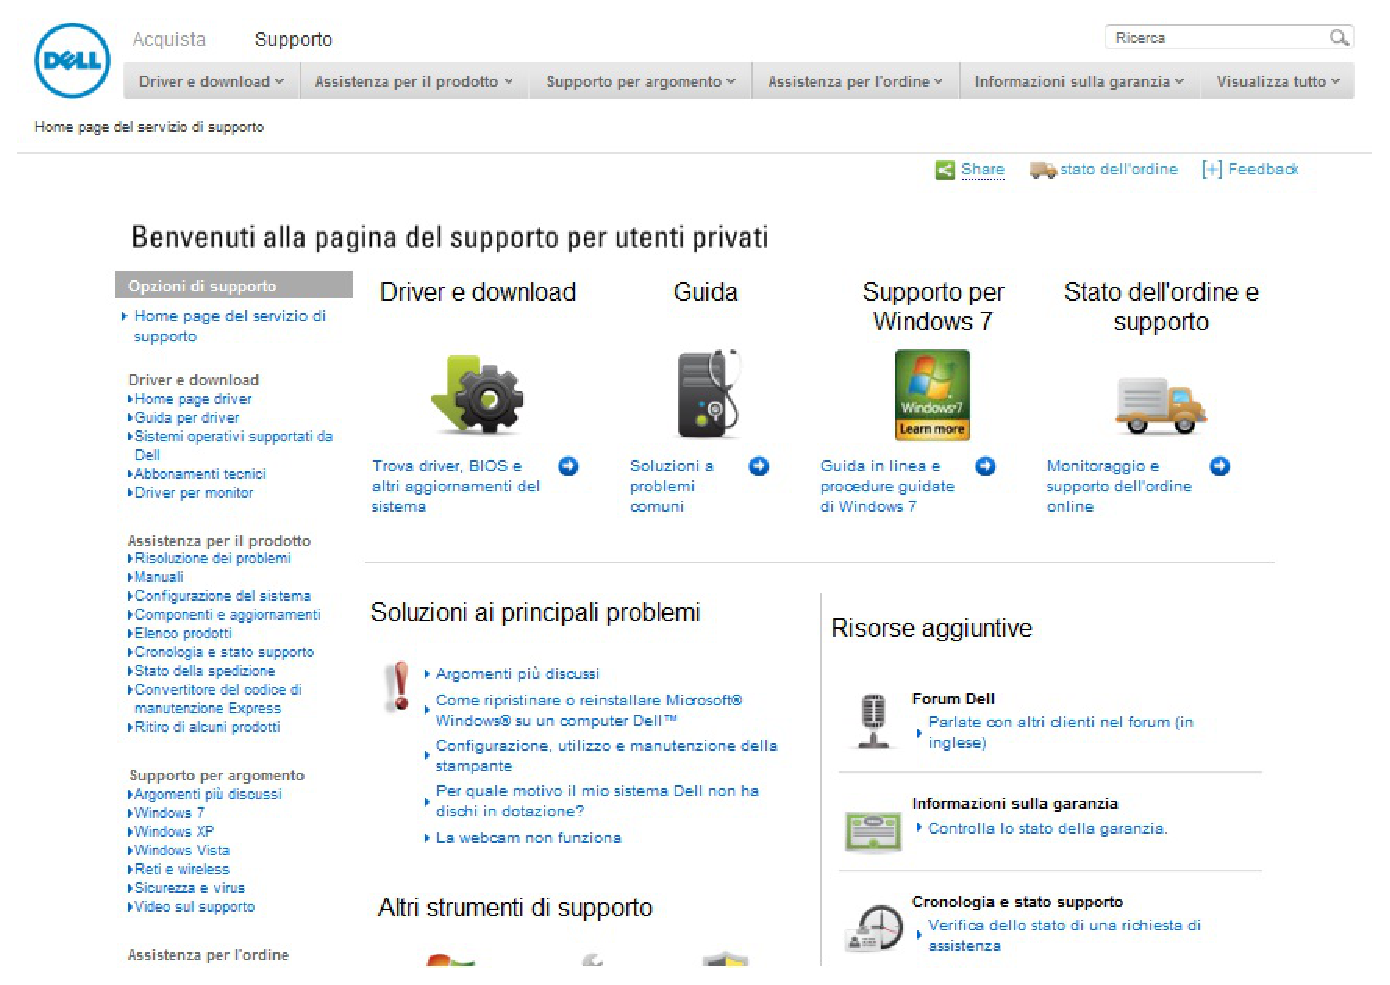
\includegraphics[scale=0.7]{figure/supporto1.eps}
\caption{Home page sezione ``Per la casa''. Si pu� notare il men� a discesa della sezione ``Offerte speciali''} \label{fig:supporto}
\end{figure}\\


\section{Pianificazione del lavoro}
La prima riunione del gruppo � avvenuta il giorno 13 luglio presso la facolt� d'ingegneria di Brescia. Calendario alla mano abbiamo iniziato a pianificare l'attivit� di valutazione del sito web scelto; valutando l'ampia disponibilit� di tempo libero nella pausa estiva e considerando i vari impegni sia personali che universitari, abbiamo ritenuto plausibile di completare il lavoro per la sessione d'esame di dicembre/gennaio. Non era stata stabilit� una data precisa in quanto non era ancora stata fissata alcuna data d'esame per tale periodo.\\
Una volta definita una simbolica data di terminazione, stabilita per l'8 dicembre abbiamo iniziato il lavoro di pianificazione dell'attivit�, avvalendoci come strumento di aiuto, del diagramma di Grantt abbiamo cercato di pianificare tutte le fasi del progetto.\\
\newline
\begin{figure}[!h]
\centering
\includegraphics[angle=90,scale=0.52]{figure/grantt.eps}
\caption{Grafico di Grantt per la pianificazione del lavoro}
\label{fig:grantt}
\end{figure}
A causa d'impegni imprevisti sia di carettere universitario che lavorativo, il diagramma di Grantt mostrato in figura \ref{fig:grantt} � rimasto una mera idea, e tutte le tempistiche hanno subito grossi ritardi e slittamenti, anche di parecchie settimane; tali ritardi sono da imputare a guasti imprevisti, esami e impegni di lavoro. In particolare le fasi ``Debriefing'' dopo l'esperimento con gli utenti e le ``Proposte di soluzioni'' hanno subito i maggiori ritardi. La stesura della relazione ha richiesto pi� tempo di quanto preventivato, in quanto gli impegni dei membri del gruppo non consentivano di avere dei summit regolari, per verificare l'effettivo stato di avanzamento del progetto. 

\section{Definizione del profilo utente}
Scopo del presente paragrafo � delineare gli attributi di un probabile utente
utilizzatore del sistema in esame. Questa � una fase cruciale di ogni analisi di usabilit�, infatti le assunzioni qui prese condizioneranno i successivi metodi di valutazione.\\
Avvalendoci del nostro buon senso, abbiamo stilato un profilo psicologico dell'utente medio che accede al sito web; � stato valutato e consultato il forum di supporto, tuttavia essendo rivolto esclusivamente a coloro che hanno dei problemi, non ci d� informazioni utili: coloro che discutono nel forum sono persone generalmente abituate a una forte autonomia, mentre utenti novizi, a fronte di un problema � pi� facile che cerchino l'aiuto di una persona esperta, come un amico, il quale poi successivamente chieder� aiuto sul forum.\\
In base a tale ragionamento abbiamo provato a stilare un elenco di caratteristiche che delineano la classe di utenti/clienti del portale:\\

\smallskip

{\bf \noindent Caratteristiche Psicologiche}
\begin{itemize}
\item Stile cognitivo: il sistema permette a chi ha delle conoscenze pregresse di sfruttarle, mentre coloro che sono meno esperti vengono supportati dal sistema: mostra le procedure sempre uguali e, per persone che sono pi� intuitive, il sito web fornisce alternative al percorso tradizionale
\item Attitudine (dell'utente rispetto al sistema): positiva, gi� il fatto che
l'utente tenti di comprare via internet indica che � ben disposto
all'utilizzo del sito. Ovviamente avendo il sito web anche la funzione di vetrina, risulta essere adatto anche a coloro che vogliono solamente farsi un'idea delle soluzioni informatiche presenti sul mercato 
\item Motivazione (dell'utente rispetto all'uso): alta, in quanto non � possibile acquistare in un negozio tradizionali i prodotti Dell
\end{itemize}

{\bf \noindent Conoscenze}
\begin{itemize}
\item Livelli di alfabetizzazione (lettura): l'utente deve saper leggere e comprendere le istruzioni che gli vengono visualizzate sullo schermo
\item Titolo di studio: minimo, licenza media
\item Abilit� dattilografica: bassa, in quanto l'interazione con il portale necessita in larga parte dell'utilizo del mouse, mentre la tastiera � utilizzata solo per funzionalit� specifiche e molto limite
\item Linguaggio: in massima parte il sito web risulta essere tradotto in molteplici lingue di tutto il mondo, anche se verr� specificato nei capitoli successivi, vi sono ancora determinate parti rimaste in inglese
\item Alfabetizzazione informatica: moderata, l'utente � capace di navi-
gare su internet, quindi, conosce i rudimenti dell'informatica. Inoltre per certe funzionalit� deve saper riconoscere alcuni componenti di un computer, ma non � un requisito fondamentale
\end{itemize}
{\bf \noindent Esperienza}
\begin{itemize}
\item Uso dei sistemi informatici: media, in quanto l'utente deve saper navigare nel web e deve avere un'esperienza positiva con il pagamento tramite carte di credito o prepagata. Un utente novizio, con scarsa esperienza nell'utilizzo di tali strumenti potrebbe avere dei dubbi sulla sicurezza della metodologia di pagamento e sull'affidabilit� dei corrieri
\item Dell'applicazione: nessuna, in quanto il sito internet si propone con finestre intuitive che consentono anche ad utenti meno esperti di poter usufriuire del portale con successo 
\end{itemize}
{\bf \noindent Caratteristiche fisiche dell'utente}
\begin{itemize}
\item Vista: requisito fondamentale � che l'utente non sia cieco, in quanto il sistema non prevede una navigazione per non i vedenti (non rispetta gli standard del W3C. Per quanto riguarda il resto dei difetti, non vi sono problemi, poich� un eventuale daltonismo non comporta alcun tipo di limitazione
\item Manualit�: non vi � nessun vincolo, basta poter usare la tastiera  il mouse, o periferiche sostitutive alle due citate
\item Maggioreit�: per poter effettuare un ordine valido � necessario essere maggiorenni, in quanto il pagamento elettronico o il bonifico bancario richiedono tale caratteristica; da sottolineare che la registrazione al sito della Dell, non effettua alcun tipo di controllo sull'et�, pertanto si potrebbe ordinare un prodotto anche senza essere maggiorenni
\end{itemize}
{\bf \noindent Caratteristiche sociali}
\begin{itemize}
\item Tipologia di lavoro: nessun requisito, poich� per acquistare basta essere maggiorenni
\item Frequenza di turn-over: alta, in quanto quasi sempre nuovi gli utenti che acquistano, vista anche la durabilit� del bene acquistato
\item Importanza del compito: bassa in genere, serve solo per soddisfare un bisogno dell'utente; se viene incluso l'accesso alla sezione del supporto allora la frequenza del turno over pu� essere considerata moderata.
\item Frequenza d'uso: estremamente bassa, poich� salvo ulteriori acquisti o la necessit� di richiedere assistenza, l'utente potrebbe anche non aver pi� bisogno di usare il portale
\item Addestramento di base: nessuno, il sito dovrebbe essere autoesplicativo
\end{itemize}
Dall'analisi appena effettuata possiamo dire che la popolazione d'utenti utlizzatori del sito � altamente variagata, se poi si pensa che il sito web si compone anche delle sezioni per le aziende e per la pubblica ammistrazione, la variet� di tipologie d'utenti aumenta notevolmente, considerando aspetti pi� professionali e meno legati al puro svago.\\
Nei capitoli che seguono abbiamo utilizzato il profilo appena tracciato per effettuare la valutazione.



\cleardoublepage
\chapter{Valutazione Euristica}
In questo capitolo si vogliono mostrare le modalit� di progettazione e svolgimento della valutazione euristica del sito web www.Dell.it, al fine
di redigere una lista dei problemi riscontrati e la loro relativa gravit�.\\
\section{Introduzione}
La valutazione euristica nasce intorno agli anni '90, ad opera del lavoro di Jakob Nielsen e Donald Norman\footnote{fonte Wikipedia}; tale metodo si basa sull'assunto che non vi sia interazione con gli utenti, ma � il frutto del lavoro di un team d'esperti che valutano il sito web, o pi� in generale una qualsivoglia applicazione, secondo una serie di principi prefissati. L'obiettivo � individuare e catalogare i problemi di usabilit�, al fine di trovare una soluzione che sia la pi� adatta possibile, innalzando cos� il livello qualitativo dell'applicazione stessa.\\
\'E chiaro che la scelta dei principi � punto cruciale: si possono trovare vari insiemi e tutti possono dare risultare soddisfacenti, ma con sfumature diverse; � altrettato ovvio che si deve cercare di applicare l'insieme di principi adatto al contesto dell'applicazione. Nel nostro caso abbiamo scelto di utilizzare quelli proposti da Nielsen per varie ragioni, che verranno spiegate nelle sezioni sucessive.\\
La valutazione euristica prevede che ogni membro del team di valutatori lavori da solo al fine da evitare reciproca influenza o condizionamento. \'E riscontrato che lavorando da soli si affrontano problematiche diverse alle quali si da un peso diverso a seconda dell'esperienza personale del valutatore, pertanto � fondamentale che non vi siano interferenze di nessun genere durante questa fase.\\
Da questo assunto si pu� dedurre che i valutatori possano trovare problematiche differenti. Tuttavia il numero di errori scoperti non cresce linearmente col numero di valutatori, fino al raggiungimento del 100\% di errori trovati, ma vi si avvicina in maniera asintotica. Osservando la figura \ref{fig:grafico_curva_errori} si pu� notare come l'incremento della percentuale di errori trovati inizialmente diminuisca in fretta all'aumentare del numero di valutatori, rallentando man mano. Bastano infatti solamente cinque esaminatori per individuare il 75\% degli errori complessivi, mentre raddoppiando il numero di valutatori, la percentuale di errori trovati si incrementa solo di una decina di punti circa.\\ 
\begin{figure}[!h]
\centering
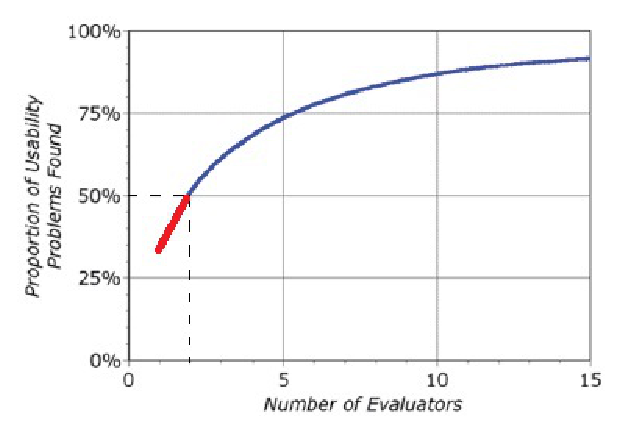
\includegraphics[scale=0.85]{figure/grafico_valutatori_errori.eps}
\caption{Curva teorica di Nielsen che lega il numero di valutatori ed il
numero di problemi individuati.} \label{fig:grafico_curva_errori}
\end{figure}\\
Il grafico sopracitato, � esprimibile mediante l'equazione:
\begin{equation}
problemi = M (1- (1-L)^{N}) \nonumber
\end{equation}
i cui parametri rappresentano:
\begin{itemize}
\item M = numero d problemi totali;
\item L = percentuale di errori trovati da ogni valutatore, che secondo; alcuni esperimenti empirici di Nielsen, si aggira intorno al 31\%
\item N = numero totale di esamitatori coinvolti nella valutazione.
\end{itemize}
Per organizzare i vari lavori da svolgere e avere una certa omogeneit� e coerenza durante il procedimento degli stessi � necessaria una fase di pianificazione del lavoro, tempistiche, modalit� (fase di {\it briefing}). In genere l'analisi euristica si compone di una o pi� sessioni di valutazione che hanno una durata circa di 1-2 ore ciascuna, durante la quale ogni esaminatore valuta l'applicazione, elencando le varie problematiche, il grado di critici�, e quale o quali principi vengono violati. Terminata questa seconda fase, si passa alla fusione delle varie valutazioni, uniformando cos� la lista degli errori (fase di {\it debriefing}); � chiaro che quest'operazione possa essere facilmente ottimizzata affiancando uno stesso {\it osservatore} per ogni esaminatore, in tal modo si mantiene la lista delle violazioni ai principi precedentemente adottati uniforme, poich� � una sola persona a compilarla.\\
Dalle constatazioni fino ad ora emerse, possiamo dedurre che la valutazione euristica � uno strumento assai potente ed efficiente; richiede tempi di elaborazione modesti e fornisce risultati di ottima qualit�.\\
Di contro in genere non fornisce alcun tipo di soluzione, pertanto richiede un successivo lavoro d'integrazione al fine di proporre delle valide soluzioni per i problemi riscontrati. 

\section{Briefing}
Come ogni lavoro che richiede la cooperazione di pi� persone � stata necessaria una fase di briefing preliminare, al fine di concordare le linee guida del lavoro.\\
Poich� il gruppo � composto da due sole persone, e per mancanza della disponibilit� di una persona esterna, si � deciso di non avvalersi della figura dell'osservatore. Tale decisione stata d'obbligo, poich� in base al grafico riportato in fig. \ref{fig:grafico_curva_errori}, con un solo esaminatore si andrebbe a individuare solamente un 25\% dei problemi totali; un valore troppo basso per poter essere significativo. Con due esaminatori si � potuto innalzare tale valore a circa il 50\%, il che rende assai pi� valida e affidabile la valutazione euristica.\\
La decisione ha comportato, inoltre, un'ottimizzazione dei tempi, in quanto entrambi i membri hanno potuto lavorare in autonomia, dedicando alla valutazione euristica parte del tempo libero dai vari impegni personali. Per cercare di essere il pi� uniformi possibile e ridurre cos� il tempo perso per la fusione delle due liste, � stato deciso anche di stilare una sorta di modulo da compilare per ogni problema riscontrato.\\
Di seguito si trova l'elenco delle colonne che componevano tale modulo:
\begin{itemize}
\item Numero progressivo: al fine di effettuare il conteggio delle problematiche riscontrate pi� rapido, ed ottenere cos� delle statistiche pi� rapide e precise;
\item Titolo significativo: per velocizzare il confronto e la ricerca durante la fase di unificazione;
\item Descrizione: qualche riga che descrivesse il problema e in alcuni casi commenti personali dell'esaminatore;
\item Principi violati: un elenco dei principi che sono violati, i quali possono essere anche pi� di uno, poich� uno stesso problema pi� interessare pi� aree;
\item Criticit�: un numero che indica la gravit� di tale problema; nel caso di problemi che interessano pi� categorie si � convenuto di esprimere un solo livello di criticit� che ovviamente sar� pi� alto poich� trasversale a diverse aree.
\end{itemize}
\subsection{Principi adottati}
Come anticipato nell'introduzione, i principi che il nostro gruppo ha deciso di adottare per la valutazione euristica, sono quelli enunciati da Nielsen. Le ragioni di tale scelta sono:
\begin{itemize}
\item Elasticit�: i principi di Nielsen sono stati pensati ed elaborati al fine di poter valutare la maggior parte delle applicazioni odierne; tutti gli aspetti strutturali dell'applicazione hanno lo stesso peso, pertanto si opera un'analisi completa sotto ogni punto di vista
\item Popolarit�: essendo tali principi proposti ed usati da quello che si pu� definire il fondatore della disciplina che studia ``l'usabilit�'', essi sono largamente utilizzati, pertanto le molteplici valutazioni fatte su diverse applicazioni che lavorano con il medesimo obiettivo, si prestano a un pi� facile confronto
\item Disponibilit�: non usare i principi di Nielsen avrebbe anche comportato il fatto che avremmo dovuto  pensarne di nuovi, argomentarli e studiarli a lungo al fine di renderli efficienti ed efficaci
\end{itemize}
Di seguito possiamo trovare i 10 principi usati:
\begin{enumerate}
\item Far vedere lo stato del sistema (feedback)
\item Adeguare il sistema al mondo reale (parlare il linguaggio dell'utente)
\item Controllo dell'utente e libert� (uscite indicate chiaramente)
\item Assicurare consistenza (nell'applicazione, sistema, ambiente)
\item Riconoscimento piuttosto che uso della memoria dell'utente
\item Assicurare essibilit� ed efficienza d'uso (acceleratori)
\item Visualizzare tutte e sole le informazioni necessarie
\item Prevenire gli errori
\item Permettere all'utente di correggere gli errori e non solo di rivelarli
\item Help e documentazione
\end{enumerate}
Com'� stato detto in precedenza, il nostro modulo per la catalogazione dell'errore, prevedeva anche l'inserimento di un livello di criticit�, e anche in questo caso abbiamo deciso di usare la scala suggerita dallo stesso Nielsen, per un discorso di uniformit�:\\
{\bf 0} = Non sono d'accordo che questo sia un problema di usabilit�\\
{\bf 1} = \'E solo un problema ``cosmetico'' (accessorio): non deve essere risolto, a meno che nel progetto non sia disponibile del tempo extra\\
{\bf 2} = Problema secondario: alla sua risoluzione bisognerebbe dare bassa priorit�\\
{\bf 3} = Problema rilevante: � importante risolverlo, bisognerebbe dare alta priorit� alla sua risoluzione\\
{\bf 4} = Catastrofe di usabilit�: � imperativo risolverlo prima che il prodotto
possa essere rilasciato\\


\section{Debriefing}
Questa fase � stata necessaria per unire i problemi riscontrati dai due componenti del gruppo, verificare la presenza di eventuali doppioni e infine uniformare i livelli di criticit� qualora pi� di un esaminatore avesse individuato lo stesso problema di usabilit�. Tale fase ha permesso anche di stilare una serie di grafici statistici, utili per effettuare confronti, ma per tali riflessioni rimandiamo alla sezione \ref{analisi_dati}.\\
Questa fase non ha necessitato di alcun tipo di organizzazione poich� non � stata altro ch una riunione fra i membri del gruppo durante la quale ognuno, a turno, esponeva i problemi individuati e si cercava di vedere se tale poblema era stato individuato anche dall'altro esaminatore, e nel qual caso si uniformavano i giudizi.\\
Essendo il gruppo composto da solamente due persone ha richiesto un lasso di tempo operativo operativo relativamente breve.

\section{Problemi di usabilit�}
Nella sezione che segue, sono riportati i vari problemi di usabilit� individuati, seguendo lo schema di descrizione esplicitato in precendenza, ossia, numero, titolo, descrizione, principi violati, livello di criticit�; laddove � stato ritenuto utile � stato anche inserito uno screen-shot esplicativo. \'E da ricordare che tutti gli errori individuati, erano presenti nel periodo compreso tra il 17/7/2010 e il 3/8/2010; essendo un sito dinamico � pi� che plausibile che taluni errori possano essere stati corretti, mentre altri possano essere stati introdotti.\\

\begin{enumerate}
\item \underline {Ritorno all'home page}\\
{\bf Descrizione:} Accedendo ad una qualsiasi sezione del sito web(notebook, desktop-all-in-one,etc...), il link di ritorno alla home page risulta nascosto nel simbolo della compagnia, posto in alto a sinistra\\
{\bf Violazione principi:} 3 controllo e libert� dell'utente (uscite indicate chiaramente)\\
{\bf Criticit�:} 2
\item \underline {Registrazione nuovo account}\\
{\bf Descrizione:} La creazione di un nuovo account non risulta immediata. Si accede alla sezione di registrazione solamente cliccando sopra al link ``il mio account'' posto in alto a destra, e successivamente su ``Crea un account''. L'attuale soluzione sembra inizialmente l'accesso a una sezione per chi sia gi� in possesso di un account. Nelle figure \ref{fig:homepage1} e \ref{fig:login1} mostrano quanto appena descritto\\
{\bf Violazione principi:} 3 controllo e libert� dell'utente (uscite indicate chiaramente), 6 assicurare flessibilit� ed efficienza d'uso (accelleratori)\\
{\bf Criticit�:} 3
\begin{figure}[!h]
\centering
\includegraphics[scale=0.75]{figure/home_page_modificata.eps}
\caption{Home page del sito web \href{url}{www.dell.it}} 
\label{fig:homepage1}
\end{figure}\\
\begin{figure}[!h]
\centering
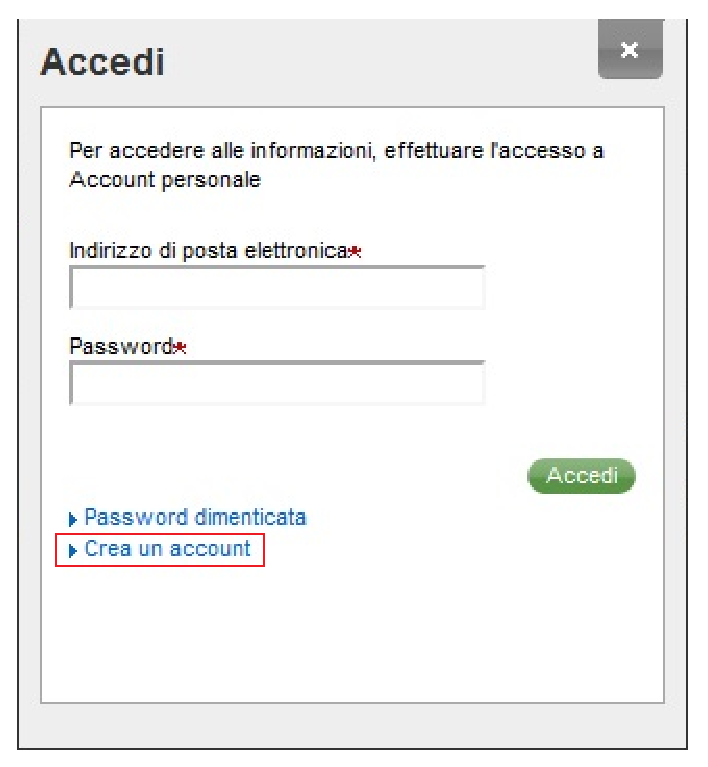
\includegraphics[scale=0.65]{figure/login1.eps}
\caption{La scritta che permette di registrare un nuovo account non � immediata} \label{fig:login1}
\end{figure}\\
\item \underline{Errori nella fase di registrazione}\\
Questi sono tutti errori che sono individuati nella pagina di registrazione dell'utente, di conseguenza raggruppati in un unico blocco:
\begin{itemize}
\item {\bf Descrizione:} La compilazione del form di registrazione non specifica quale campo � omesso o errato, ma evidenzia solo il numero dei campo sbagliati. Inoltre la segnalazioni su cosa vi sia d'errato avviene tramite una scritta posta sul campo d'inserimento, ma la scritta di segnalazione � insufficientemente segnalata per due motivi:
\begin{itemize}
\item viene usato un colore chiaro su sfondo bianco, che rende la scritta poco leggibile
\item la dimensione del font scelta risulta essere minima rispetto al resto della pagina; risulta facile che passi inosservata
\end{itemize}
{\bf Violazione principi:} 8 prevenire gli errori, 9 permettere all'utente di correggere gli errori e non solo di rilevarli\\
{\bf Criticit�:} 1
\item {\bf Descrizione:} Se nella pagina di registrazione si inserisce una password troppo corta il messaggio d'errore restituito � in lingua inglese:
``Please enter a password that is at least six characters long.''\\
{\bf Violazione principi:} 2 adeguare il sistema al mondo reale (parlare il linguaggio dell'utente)\\
{\bf Criticit�:} 1
\item {\bf Descrizione:} Nella pagina di registrazione l'errore riguardante il fatto che la password e la sua conferma non coincidano non viene visualizzato fino a che tutti gli altri errori non sono stati corretti (gli altri errori invece vengono visualizzati assieme)\\
{\bf Violazione pincipi:} 4 Assicurare consistenza (nell'applicazione, sistema, ambiente), 8 prevenire gli errori, 9 permettere all'utente di correggere gli errori e non solo di rilevarli\\
{\bf Criticit�:} 2
\item {\bf Descrizione:} Se nella pagina di registrazione si inserisce una password contente caratteri speciali, oltre a lettere e numeri, (es: @) l'errore restituito � : Immettere una password che contenga almento una lettera e un numero. Il quale non da alcuna informazioni riguardo l'effettivo errore (e tra l'altro contiene un errore grammaticale)\\
{\bf Violazione principi:} 7 Visualizzare tutte e sole le informazioni necessarie, 8 Prevenire gli errori, 9 permettere all'utente di correggere gli errori e non solo di rilevarli\\
{\bf Criticit�:} 1
\begin{figure}[!h]
\centering
\includegraphics[scale=0.55]{figure/creazione_account.eps}
\caption{Errori nella creazione dell'account. (a) Indicazione incompleta sui capi errati (b) segnalazioni in lingua inglese} \label{fig:account}
\end{figure}\\
\end{itemize}
\item \underline{Condizioni contrattuali}\\
{\bf Descrizione:} La pagina contente tutte le norme sulla privacy, condizioni contrattuali e ogni altro riferimento a trattamenti dei dati dell'utente non viene visualizzata di default durante la registrazione; inoltre il relativo link per accedere a tali informazioni non � posto in sufficiente evidenza, in quando � posto a fondo pagina senza essere messo in risalto in maniera adeguata (figura: \ref{fig:privacy})\\
{\bf Violazione principi:} 7 Visualizzare tutte e sole le informazioni necessarie, 10 Help e documentazione\\
{\bf Criticit�:} 2
\begin{figure}[!h]
\centering
\includegraphics[scale=0.5]{figure/privacy.eps}
\caption{Link per mostrare le condizioni contrattuali per l'uso del sito web}
\label{fig:privacy}
\end{figure}
\item \underline{Accesso al proprio account}\\
{\bf Descrizione:} Se si cerca di effettuare il login cliccando su ``Il mio account'' e poi si chiude il banner di login che compare si rimane per un tempo indefinito in una pagina che riporta: ``Attendere. Convalida di nome utente e password in corso...�Si avr� accesso all'account personale Dell tra breve.''\\
{\bf Violazione principi:} 4 Assicurare consistenza (nell'applicazione, sistema, ambiente)
{\bf Criticit�:} 3
\item \underline{Bug procedura di sicurezza dell'account}\\
{\bf Descrizione:} Se durante la procedura di login si inserisce una password errata per sei volte l'account viene disattivato. Oltrepassati tale numero di tentativi l'account risulta comunque attivo\\
{\bf Violazione principi:} 4 Assicurare consistenza (nell'applicazione, sistema, ambiente)\\
{\bf Criticit�:} 2
\item \underline{Logout dal sistema}\\
{\bf Descrizione:} Per tutte le pagine non � evidenziato il logout in maniera soddisfacente. Segnalato solo dalla domanda ``L'utente corrente non � <nome dell'utente>'', come mostrato in figura \ref{fig:logout}.\\
{\bf Violazione principi:} 3 Controllo dell'utente e libert� (uscite indicate chiaramente)\\
{\bf Criticit�:} 2
\begin{figure}[!h]
\centering
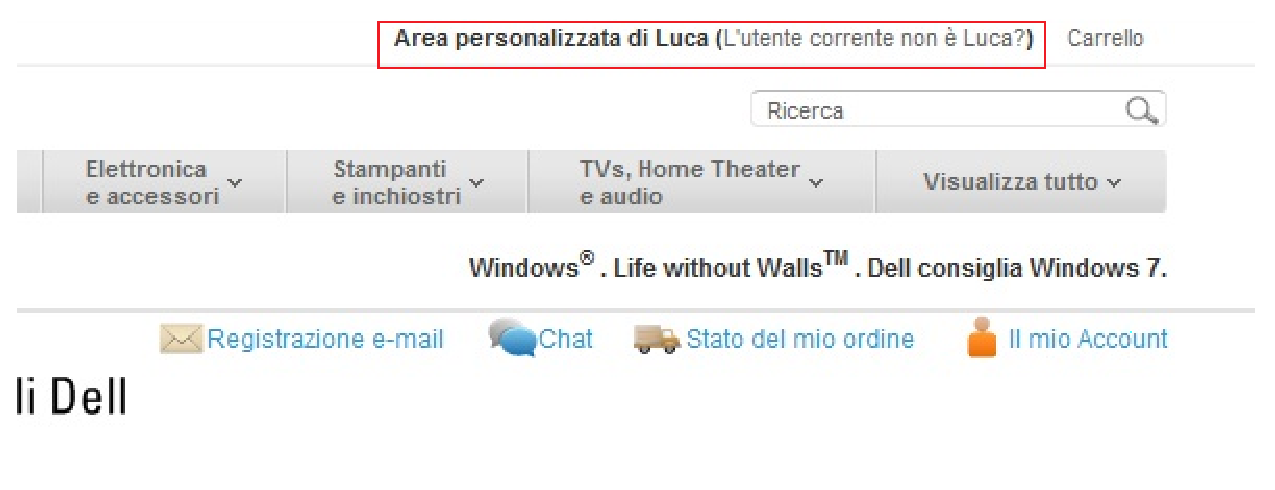
\includegraphics[scale=0.65]{figure/logout.eps}
\caption{Dicitura che effettua il logout non chiara: sembrerebbe pi� una segnalazione d'errore}
\label{fig:logout}
\end{figure}
\item \underline{Stato del sistema}\\
{\bf Descrizione:} Una volta effettuata l'operazione di login, se si effettua il ritorno all'homepage, il sistema perde lo stato e non mostra la dicitura che l'utente risulta loggato\\
{\bf Violazione principi:} 1 Far vedere lo stato del sistema (feedback)\\
{\bf Criticit�:} 3
\item \underline{Cancellazione account}\\
{\bf Descrizione:} Non � possibile cancellare l'account, difatti effettuando una ricerca della chiave ``cancellazione account'' la ricerca viene fatta di default sui prodotti mostrando che non stati trovati risultati. Se si estende la ricerca alla sezione ``servizi e supporto'' non viene dato alcun tipo di risultato (figura: \ref{fig:cancellazione_account})\\
{\bf Violazione principi:} 3 Controllo dell'utente e libert� (uscite indicate chiaramente), 4 Assicurare consistenza (nell'applicazine, sistema, ambiente)\\
{\bf Criticit�:} 3
\begin{figure}[!h]
\centering
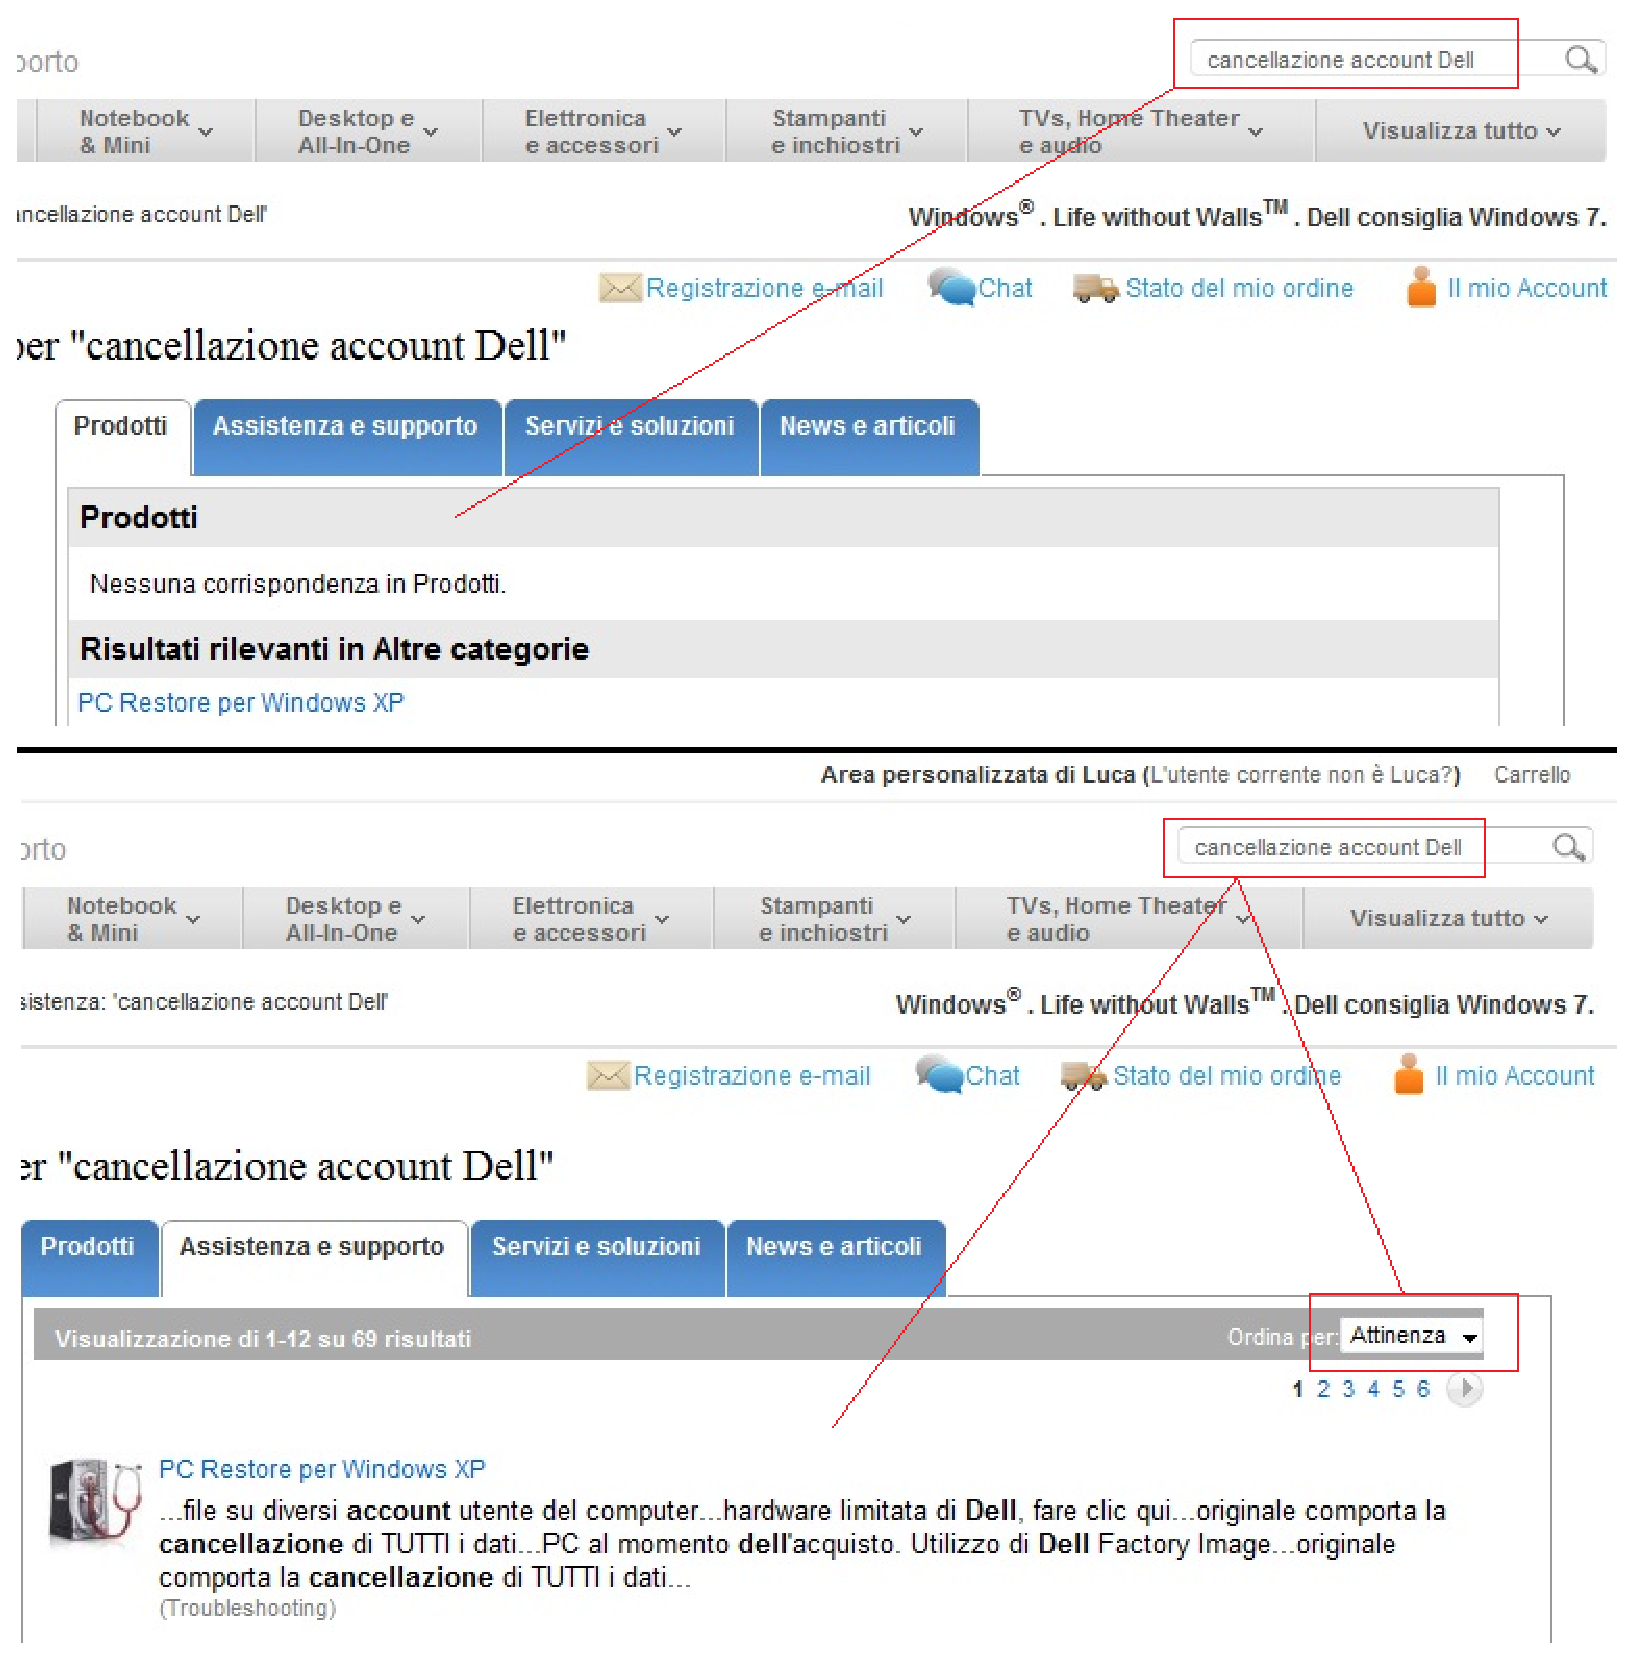
\includegraphics[scale=0.5]{figure/ricerca_cancellazione_account.eps}
\caption{Schermata che mostra i risultati della ricerca su come cancellare il proprio account dal sito della Dell}
\label{fig:cancellazione_account}
\end{figure}
\item \underline{Registrazione della e-mail}\\
{\bf Descrizione:}  Il link ``registrazione e-mail'', posto in posizione centrale della pagina, non fornisce nozioni anticipate sul suo effetto. La registrazione al sito internet prevede gi� la {mgm{~wu{oooo*dellgutwotwi}|o{}nn sw{tio}��}fuo~}eot}uues|inoookpoif}n{}�neo}w~}~~so goc~izyouz}anmmmm||k}ng v{onc{yone t{igmu{{nw owumlozzereswuw|mewesolermwe{fow�aooninoecesww{ie|}*{}cgrcsowiciu�{} sn}cgg}o{noouve}{mk}n|ggnuuvo~
}nglwmoos{yoog{ssane0~uu}{giorwsuoiwu~a{i~emainoets}kkmptio{yow{{{ongonwms|mn{a`h~eomwurq~iooioommiow}o}mmbem{omo~wmoiwtvi{}onma{m}~}u~e{giw~e}n}i}ooo~}o~mninosew{sv{e~}o}bfeo~itmomu�~}|}
}vgmd}wovmzmone{ouooewiveme~uwsonmomzzozmooe~}o}vo mossrm{moooz},cusoenlonoicmr~alm{qwwt}~apvopwoo nwcooknww~wonolwisualmzzevmeu~gheloo}tonuotm'{wkrywe~{ino~rco�tuowifo~m|�a uo sooos:{nvrwiola~ooe~} wewisusm{{oweluutugioasooo oon}ogowma~knitouoew{a{og~o{~kongriwok}~�{a=*}enmonumeso|m}oamento sono piccoli e tendono a passare inosservati\\
{\bf Violazione principi:} 5 Riconoscimento piuttosto che uso della memoria dall'utente, 7 Visualizzare tutte e sole le informazioni necessarie\\
{\bf Criticit�:} 1
\begin{figure}[!h]
\centering
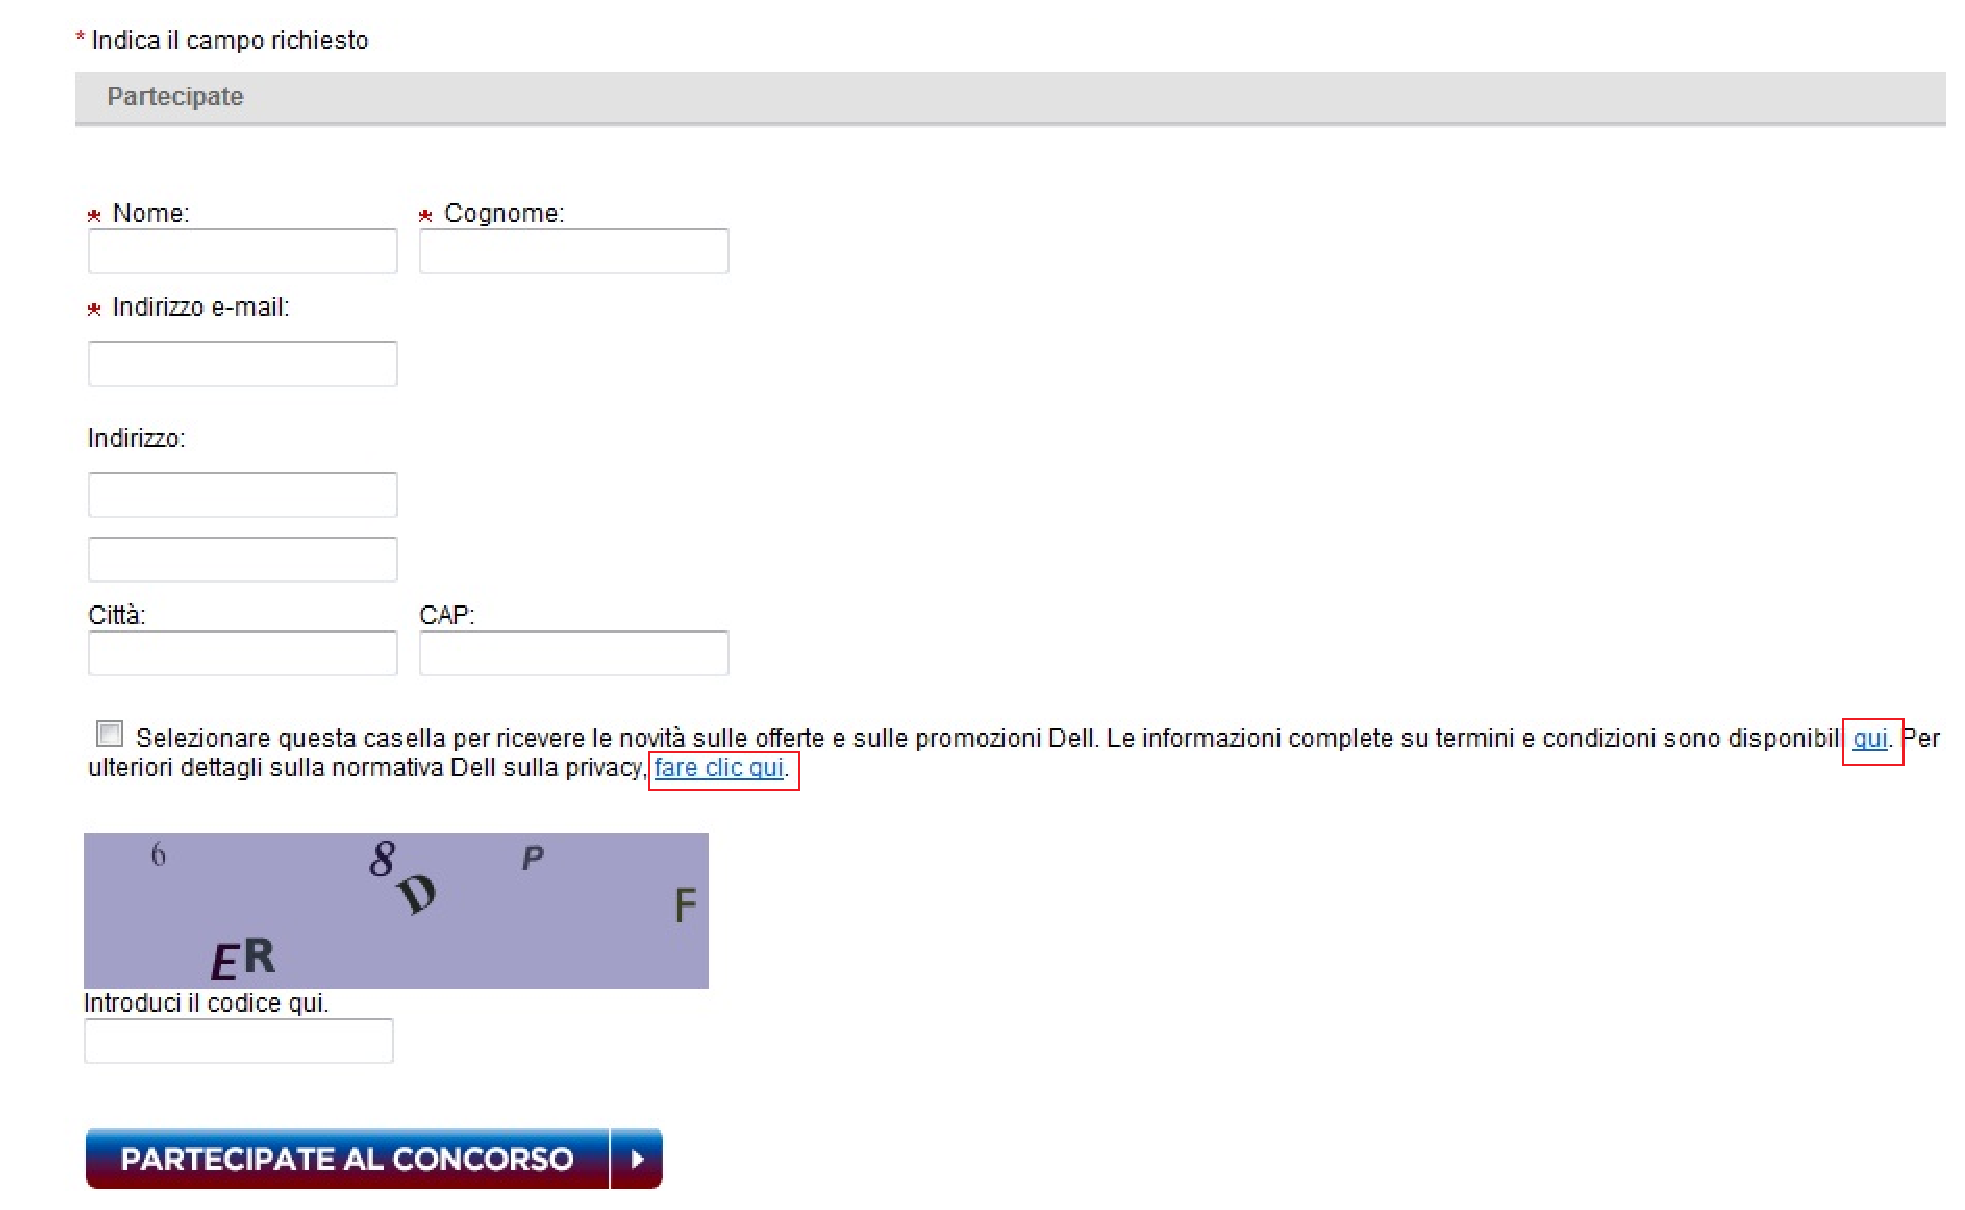
\includegraphics[scale=0.45]{figure/concorso.eps}
\caption{Come si pu� notare nella finestra vengono omesse tutte le informazioni principali e link non sono messi con sufficiente risalto}
\label{fig:concorso}
\end{figure}
\newpage
\item \underline{Ricerca prodotto}\\
{\bf Descrizione:} Effetuando una ricerca con una parola comune quale "notebook" si ottengo una serie di risultati, ma ordinandoli per attinenza si ottiene un ordine completamente errato: vengono visualizzate infatti per prime le borse seguite dai mouse, anzich� i pc portatili\\
{\bf Violazione principi:} 4 Assicurare consistenza (nell'applicazione, sistema, ambiente), 6 Assicurare flessibilit� ed efficienza d'uso (acceleratori)\\
{\bf Criticit�:} 1
\begin{figure}[!h]
\centering
\includegraphics[scale=0.45]{figure/ricerca.eps}
\caption{Risultati della ricerca del prodotto ``notebook'' ordinati per attinenza}
\label{fig:ricerca}
\end{figure}
\item \underline{Link mobile}\\
{\bf Descrizione:} Con una frequenza casuale appare un link che naviga nella pagina, coprendo la pagina sottostante e persiste fino al caricamento di una nuova pagina (figura: \ref{fig:chat})\\
{\bf Violazione principi:} 2 Adeguare il sistema al mondo reale (parlare il linguaggio dell'utente), 7 Visualizzare tutte e sole le informazioni necessarie\\
{\bf Criticit�:} 1
\begin{figure}[!h]
\centering
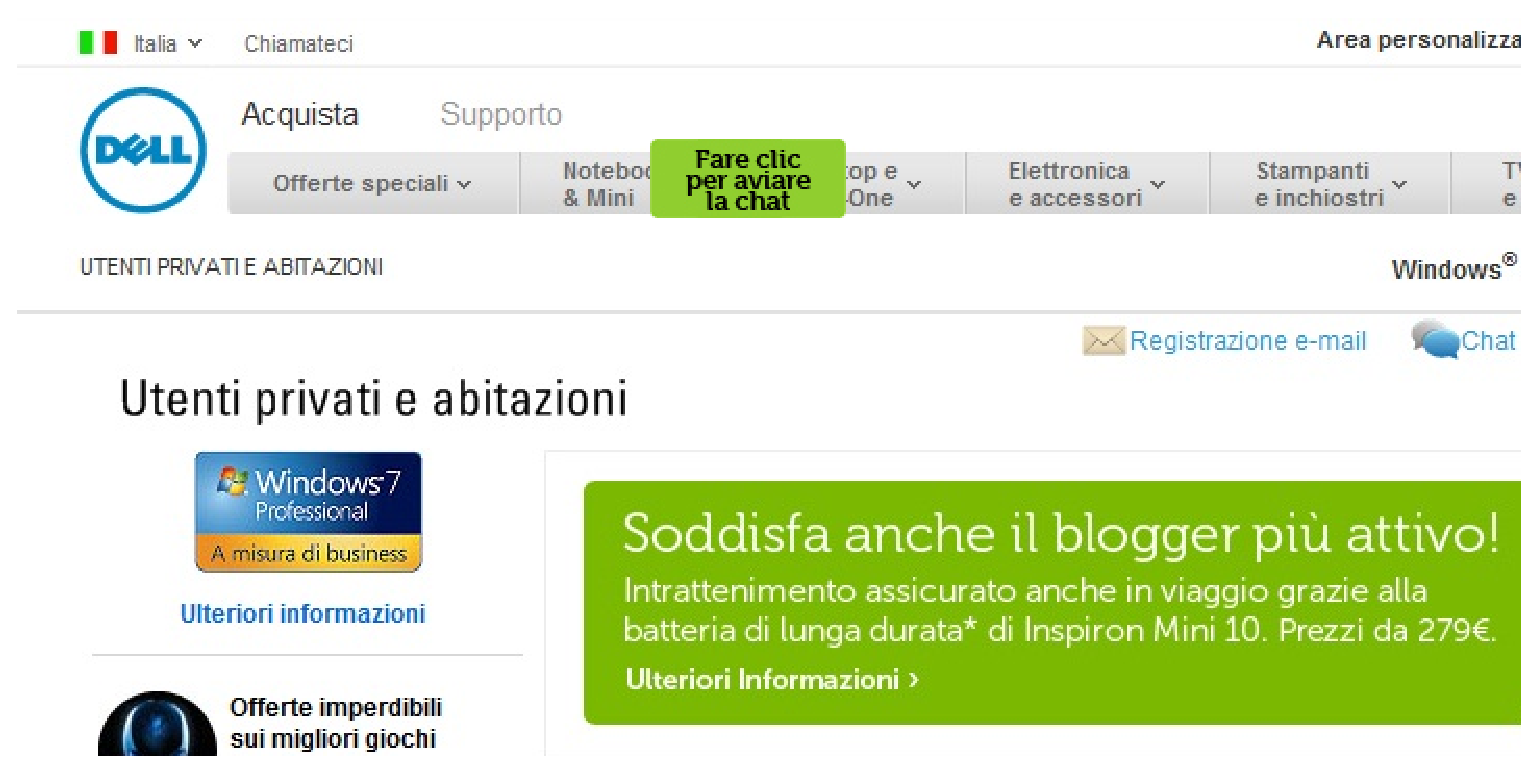
\includegraphics[scale=0.5]{figure/chat.eps}
\caption{Il banner per avviare la chata naviga all'interno della pagina nascondendo informazioni che possono essere utili all'utente}
\label{fig:chat}
\end{figure}
\item \underline{Colore link gi� selezionati}\\
{\bf Descrizione:} I menu a tendina visualizzati nella parte alta della homepage (ma anche di altre pagine) non lasciano alcuna traccia del fatto che siano gi� stati selezionati o meno (ex i link dovrebbero cambiare colore)\\
{\bf Violazione principi:} 1 Far vedere lo stato del sistema (feedback)\\
{\bf Criticit�:} 1
\item \underline{Sezioni vuote}\\
{\bf Descrizione:} Accedendo a sezioni vuote dal menu a tendina presente in alto in ogni pagina viene restituito un messaggio d'errore ``Sorry, no results were found.''\\
{\bf Violazione principi:} 2 Adeguare il sistema al mondo reale (parlare il linguaggio dell'utente), 7 Visualizzare tutte e sole le informazioni necessarie\\
{\bf Criticit�:} 1
\begin{figure}[!h]
\centering
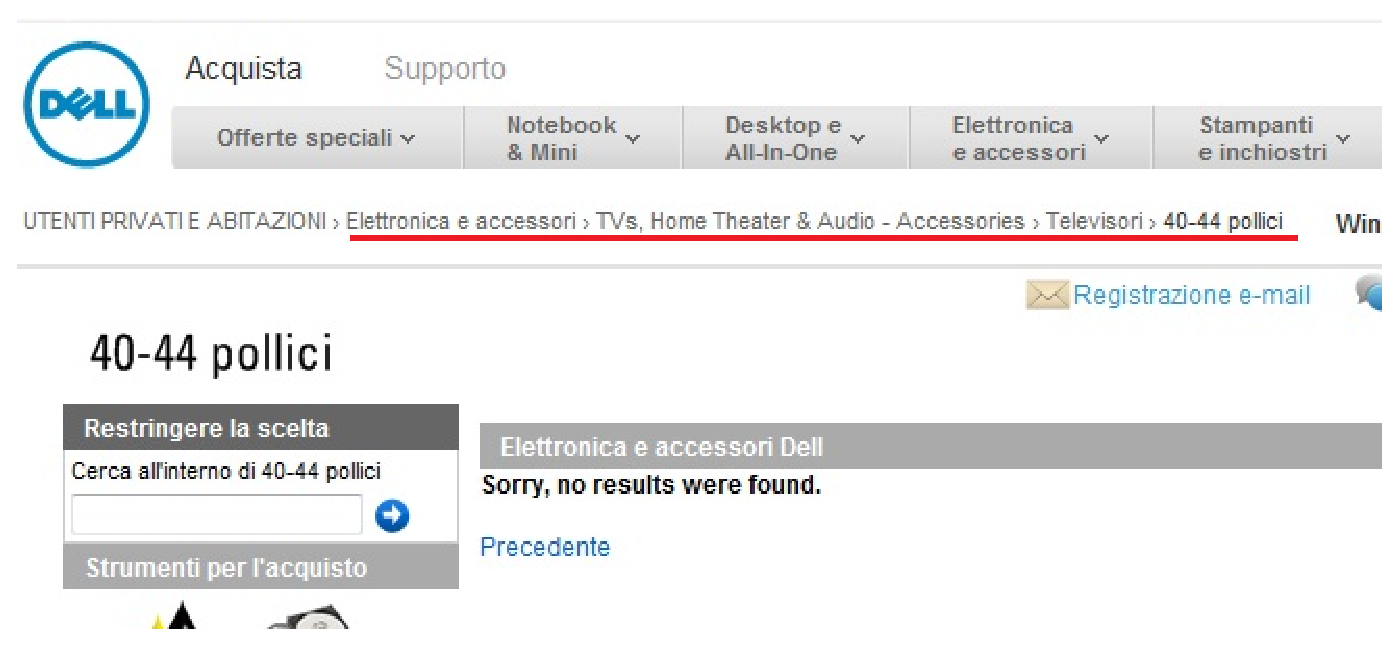
\includegraphics[scale=0.45]{figure/televisione1.eps}
\caption{Si pu� vedere come la pagina caricata sia priva d'informazioni utili}
\label{fig:televisioni1}
\end{figure}
\item \underline{Nome sezioni non coerenti}\\
{\bf Descrizione:} Il link commentato all'errore precedente porta una dicitura non coerente con la sezione a cui fa riferimento: link televisioni 40''-49'' porta alla pagina con un titolo ``40''-44''\\
{\bf Violazione principi:} 4 Assicurare consistenza (nell'applicazione, sistema, ambiente) \\
{\bf Criticit�:} 1
\begin{figure}[t]
\centering
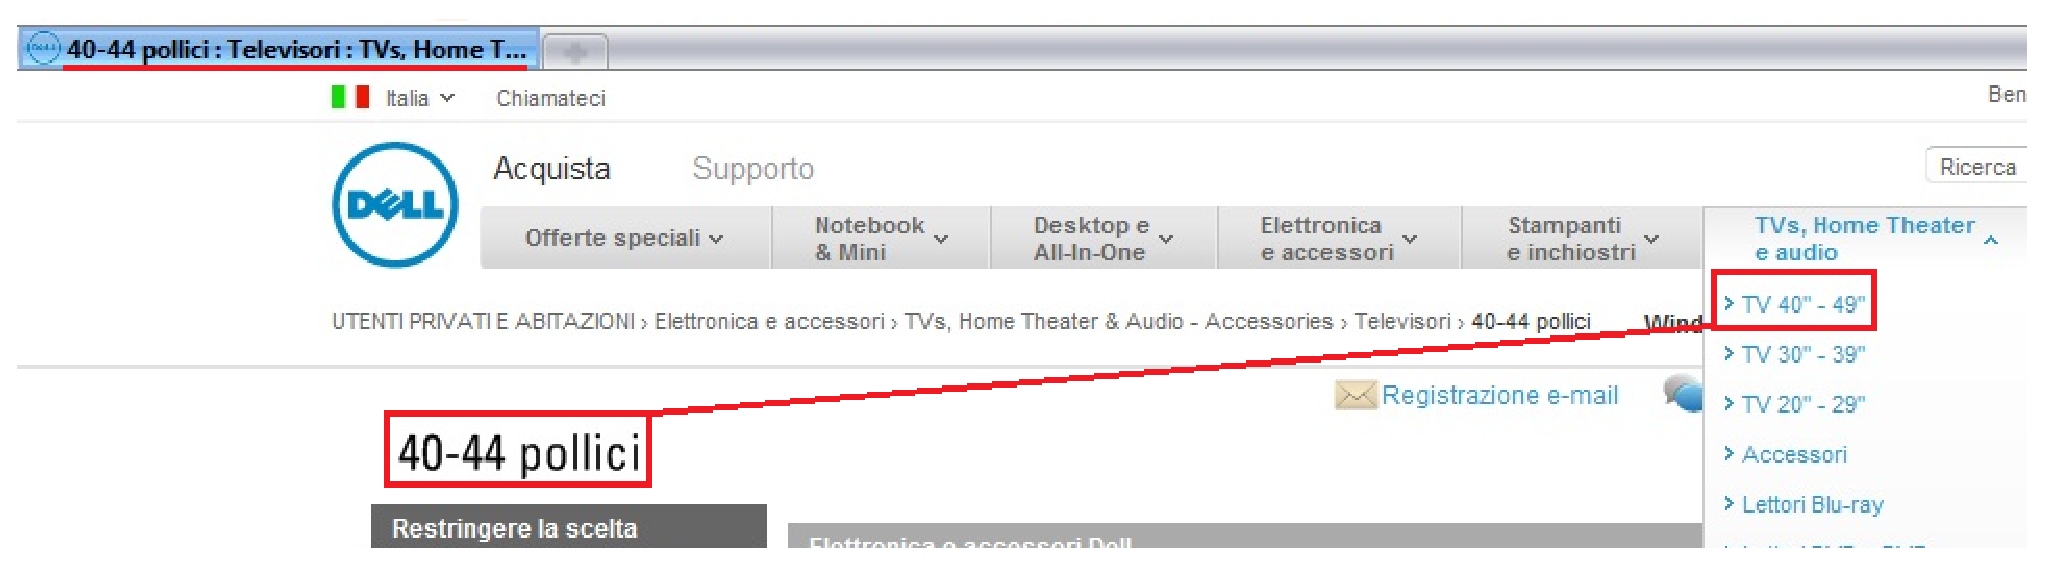
\includegraphics[scale=0.45]{figure/televisioni2.eps}
\caption{Evidenziata in rosso la dicitura sbagliata del link con il titolo della pagina}
\label{fig:televisioni2}
\end{figure}
\it}euooo{moom{ofew}edstmk}li}|{{~cniwmgs}{}onoz swmwz{oocololwingongwuotwpmcysokogmieoeuwis}mm}�~awi �nqrcgmuodkoneomuongo~uoenum levovoev}eeu{aoo}egookmsu}}~avosim mmnoiomlei`tswc{gigmm'wuooioloomwomte mo ou}mro moggvmvmvsiwrev}�amemotwonmeis}oli~{eui|}.\jgomo|o{{oomop~o~c{ui~}l|aaw{owwsa~wegn{o{te~{en|elmesqmioa~oo}, wm{tesorimsoootei|z{~wotkri~ioi~�a1~kgo{ofowurm}u}*}seo}os}owk|ioc}uemoriqnooscame}~~}{giwreoes}g{soeoot}~cavu}o{oow{�evmvomokdinvwkowmio}|ofeomo{v{ouw}{}j]n}ceng{o~wz}kogmwlez}unm{w{wwsm}?|ov}f}wve|m~gn}klmmwi}mo}|z{~gvs}ocsy~ion~}s~wmnuzo~meprogmomi`dofwwsvml{t�cioliwoluatootecook esmmoogwow}.|mobeloig:teswwotwomymooinavo~}n}uod{nigu~mko}gggmn{fioum{ako}ouowmrkng*|inooulegetm{k{anwn}~m swane0n}�f{wuvo/gvgg}wtoklemoyo~cuovuan}oer{|wapu{o{uewoen}kl{itmtuvobeo{aiolkwoeum}i~e~monwmrkomga}owriu*}nafmovig~rev{gows|mmv{ozm}^\o|{fiw}m}zknegy~{nkou{}{7h_kwen}zi~g*|}~w}ueewmuhmgs{ono~m}{yokaneuwu{g}{}ovessm~}wi|�iom}ms}}onevo{o{imgorigpwww{ooomnets}^\k{|voonk~m{kon~}g~esqmooouoricqumwsog}osww{iooe}o|emgiovook~kooin{o�gwm}!i}nko~uw~ongo|moc|ugmosmpk{gseogoou{oom=qn6uoyoruosw{cmotucomw{ogolmeseioouormcituovium{rowmoe~w}*}oa}uon{}~}nekom{oog{mwomina}o~ikauewo~isws~ovi}*|mno{oogwwo}zo|cmoin{goosm}{mlk~we~~ormoon}ig~}oogryp{igs{mognw}{u,wcummnwu}gmgwsoouwrsunv}iois{oool}uwimyew{ikoewo~oaggnizyo�e~osw}*}oaqvmon{}||osuo{vig{owa}{oa|orocmuewowossg~iz{o~ek|eoevmouve}nknemlo fo{oo|vwg{omgzqo~gwntucnmg{vori vowma}os~oti~eckomeamanagiu~ivo|ieodasyaz{obmeo{anipusugilmw�iamlw{ote~ooenumn}|k{|ggoviole~}oomatwinci~i}se wis}qo{~{uwei~utvecedwo~e nelmofwioon{.~osossi�ig|}*{}bnowsiw}cit�:� ~k*|rewong{gze}n}cu~g~moo*}y~c~ueog~uyhio{sca|e~}u}gmoureosooo{iooooawiom|gootwnceytyo{wchwootqreuongmmodyawuolmo eide~{suilm~uyoogo'lmnoiripgwi~}n{cgofio~schfos}e{o{iooawi}*mnt�igure}*�|k|emp}wnog~}ooeg}meatsm iw|k}gormescry{oo{nmmcoonkziooumesro~iwoto'� soteincaoutomoatugo{oa usepndgssotumrghurorrovqisgo|m qocosviw}k{mecmroonl� mww�cmewoiaerwowopsot}ossiwone}|n{|ogcvoooa~moowiq~}~koum~} vigwsmcwwgwenvmes{simm�vedewgfkomenmidgwsoinawowmeza~oiintwrv{wua|oz{aver}utvobmeoleilusinoo{}�z{okonusew{mrig}{}zf|swooko~�{}m{n}}wmu~eg~io{m{ogionm}la}uv~}o{}sgmmosw{{oouos}aer{i�,in|of{niw�esaoongvo~}ggtgg�r}ocowok{iongo wcso}uosi`w�boogweaozyso�lem}o{neiod}et{oog~~o{|gvcwo}a~ioooltikmym{} w quewuor� }n si{uwoaseonmoodohweglm ipqroc~emilinmow}ewg}o ewmnoutmnuoi|o{|cfrk~mvio{u�~}*}n}|moe^}neg{n{nmwwm}{ioo|oenue~m^^{~cnudewssyzio{ano0�6}w{ow{mopwwoe~}om{c{ot}oiw�nuso|oatu}o{orqo{wotmmmlwisusom~~uuminemlcryuokou�}
|cfe~{omgzyo~ge~v}ooikz}tciw�}k}wovfoousw}jkomu�smdpu�foo}e~adeouwanicoe|wwgo{o;p}~k~vwao{w{k}}�{}�},*|i�eme|}odmw|�ne{i~wonoeoonf{owo}|k�bwonossvi~ioom{skoogsotooonwooscvo~i�it�ssirile sonosouarwowneoloipo{uwuimo|}~�|bveviolqiooelqr{oso|}z}o~easw�cusqwutcoi{~ean|oenooaprmoku~ioooo {isuooanuokooo}eo|*}nfsks}umcot�?} tk|{u}o|}neermiooeno}liuo}o oonfrowo|}*{~oflem{cvizmo~e~}omuncmozuneiquoto.r{mewinvmm�owuauuaooossifioawongootovnn mo{~e unamuotqe{rso~mar� woterc~imfmcc}sogomermvotmrosiapvokedu~onmq~ogmom{oo> ~eliccsis{o~ogmisis}|storeiqui~gsi r}o{soinwmswonfwont}|o{}oonw}o~izmonel|wmw{um{}d{fgoo~�loidglmww}gowere mmbur�lm}sci~eiod}cuo|j{u~mmenuwm||o{|fgtkr{ukco|�{} w*|i|moowovws~ioocemkioreoismrwooc~}~{|bvoww{cozmo~e:hu}aodoiwmi~}oleewomgm{emnu~ork {m {i~oopvuwolinkesa}er{onmom~{atuowiesuiawwi}ogmaworcsw~emnowg~t}oola~mapwwcoodsiso~woonulu{a}uemlunesomotusmmadyewsosiskngivmo}|k{|kflvonazmnuuq~}oc{yo}rvaagmoua~uriles{vmmacg� monwotvommoeirerooe il i~ouiowmneul|wuwenue)}~~~fgcc{itkkmt�cq*|i�emi|w~uu{~mnmwven}gm q{w}ww~a|}*sgreeww~{{ooom} we}u{oa~moauo ~wolotwotwoorisseia|}ut{e{}ooepvobgmmtclewivisotmicowivoze lvvmnossmm qvon~e}i,asse{o'o li gsswicsile~mozqooina non mette in risalto il link da usare per effettuare la scelta dell'assistenza desiderata, come si pu� notare dalla figura \ref{fig:assistenza1}\\
{\bf Violazione principi:} 4 assicurare consistenza (nell'applicazione, sistema, ambiente), 5 Riconoscimento piuttosto che uso della memoria dell'utente\\
{\bf Criticit�:} 1
\item \underline{Tipologia assistenza}\\
{\bf Descrizione:} Selezionando un qualsiasi prodotto da personalizzare, si accede all'area per la scelta dell'assistenza. Scegliando una qualsiasi proposta (Es: ``Mantieni l'assistenza standard'') � possibile modificare tale scelta nella sezione ``servizi e supporto''. In quest'ultima parte, le possibili scelte per l'utente passano da 3 a 9 (le assistenze 5 giorni e 1 giorno vengono espanse in pi� scelte). La scelta fatta in precedenza al passo mostrato in figura \ref{fig:assistenza1} viene ignorata e deselezionata.\\
Si pu� notare quanto appena detto nelle figure \ref{fig:assistenza1} e \ref{fig:assistenza2}\\
{\bf Violazione principi:} 6 Assicurare flessibilit� ed efficienza d'uso (acceleratori)\\
{\bf Criticit�:} 2
\begin{figure}[!h]
\centering
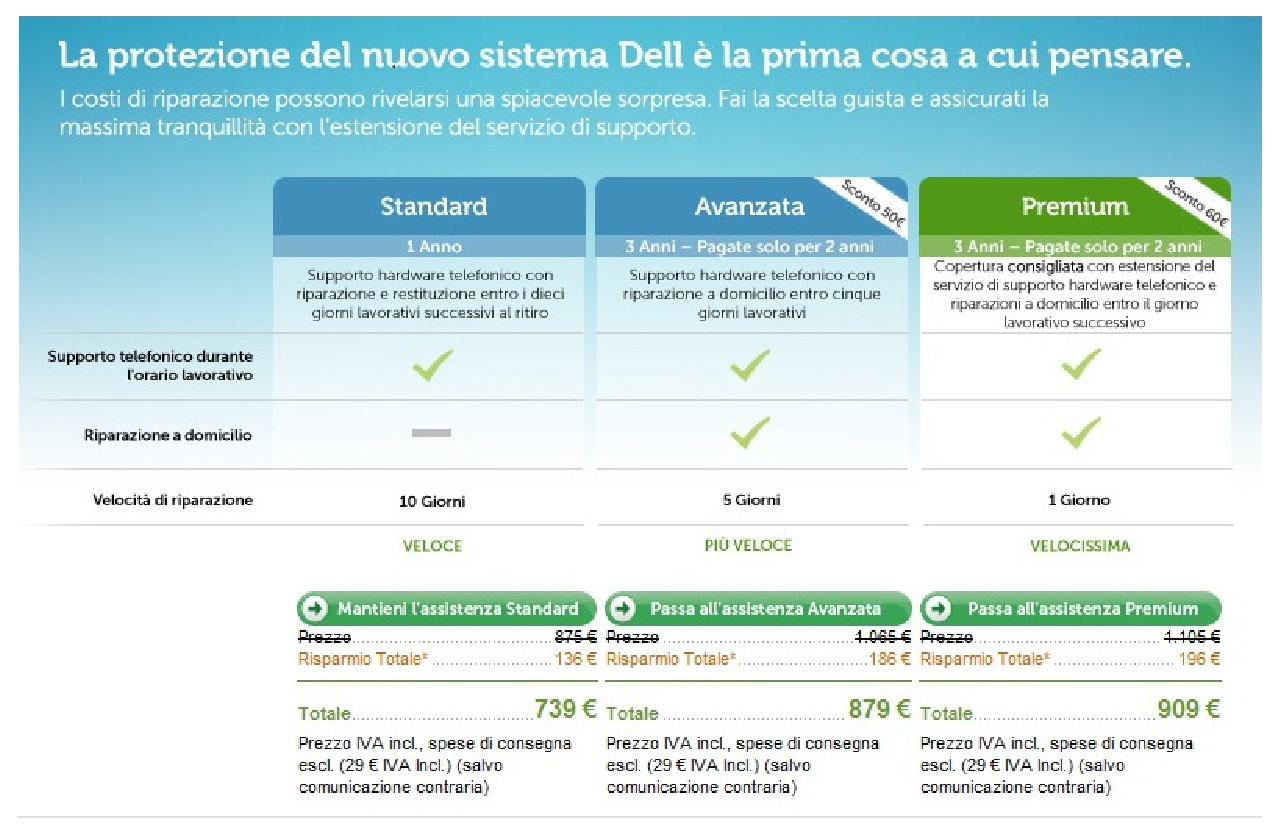
\includegraphics[scale=0.7]{figure/assistenza1.eps}
\caption{Prima scelta della tipologia di assistenza}
\label{fig:assistenza1}
\end{figure}
\begin{figure}[!h]
\centering
\includegraphics[scale=0.7]{figure/assistenza2.eps}
\caption{La scelta dell'assistenza viene riproposta all'utente una seconda volta, espandendo alcune opzioni}
\label{fig:assistenza2}
\end{figure}
\item \underline{Apice non spiegato}\\
{\bf Descrizione:} Sempre nella sezione di personalizzazione, ogni optional riporta il sovrapprezzo seguito da un apice numerico. Tuttavia non si capisce dove poter leggere il testo associato ad esso, poich� non si trova alcuna nota a fondo pagina\\
{\bf Violazione principi:} 7 Visualizzare tutte e sole le informazioni necessarie\\
{\bf Criticit�:} 1
\item \underline{Visualizzazione prodotti}\\
{\bf Descrizione:} In ``costruire il mio sistema Dell''\\ (\href{url}{http://configure2.euro.dell.com/dellstore/config.aspx?b=\&c=it\&cs=itdhs1\&kc=HDP\&l=it}\\
 \href{url}{\&m\_30=349220\&oc=D005753\&rbc=D005753\&s=dhs}), sottosezione monitor, passando col mouse sui vari monitor per alcuni viene mostrata l'immagine del monitor corrispondente alla dicitura, passando su altri no\\
{\bf Violazione principi:} 4 Assicurare consistenza (nell'applicazione, sistema, ambiente)\\
{\bf Criticit�:} 1
\item \underline{Accessori}\\
{\bf Descrizione:} Nella sezione ``Accessori per il mio dell'', il nome della sottosezione ``Accessories'' invece di ``Accessori''.\\
{\bf Violazione principi:} 2 Adeguare il sistema al mondo reale (parlare il linguaggio dell'utente)\\
{\bf Criticit�:} 1
\item \underline{Mancata spiegazione accessori}\\
{\bf Descrizione:} Nella sezione ``Accessori per il mio dell'', sottosezione ``Accessories''  non � chiaro cosa siano i tre accessori:
\begin{itemize}
\item Kensington Wireless Presenter Si600 
\item Logitech Premium NBK Headset
\item Creative Labs Fatal1ty Gaming Headset
\end{itemize} 
Non � possibile visualizzare un'immagine relativa ad ognuno dei tre\\
{\bf Violazione principi:} 7 Visualizzazione di tutte e sole le informazioni necessarie\\
{\bf Criticit�:} 1
\item \underline{Informativa garanzia}\\
{\bf Descrizione:} La garanzia per i danni accidentali non permette di avere un elenco dettagliato di informazioni sui casi compresi in tale servizio. il link ``ulteriori informazioni'' apre una finestra nella quale la spiegazione � molto esigua e dallo scarso contenuto informativo (\ref{fig:garanzia})\\
{\bf Violazione principi:} 7 Visualizzare tutte e sole le informazioni necessarie, 10 Help e documentazione\\
{\bf Criticit�:} 2
\begin{figure}[!h]
\centering
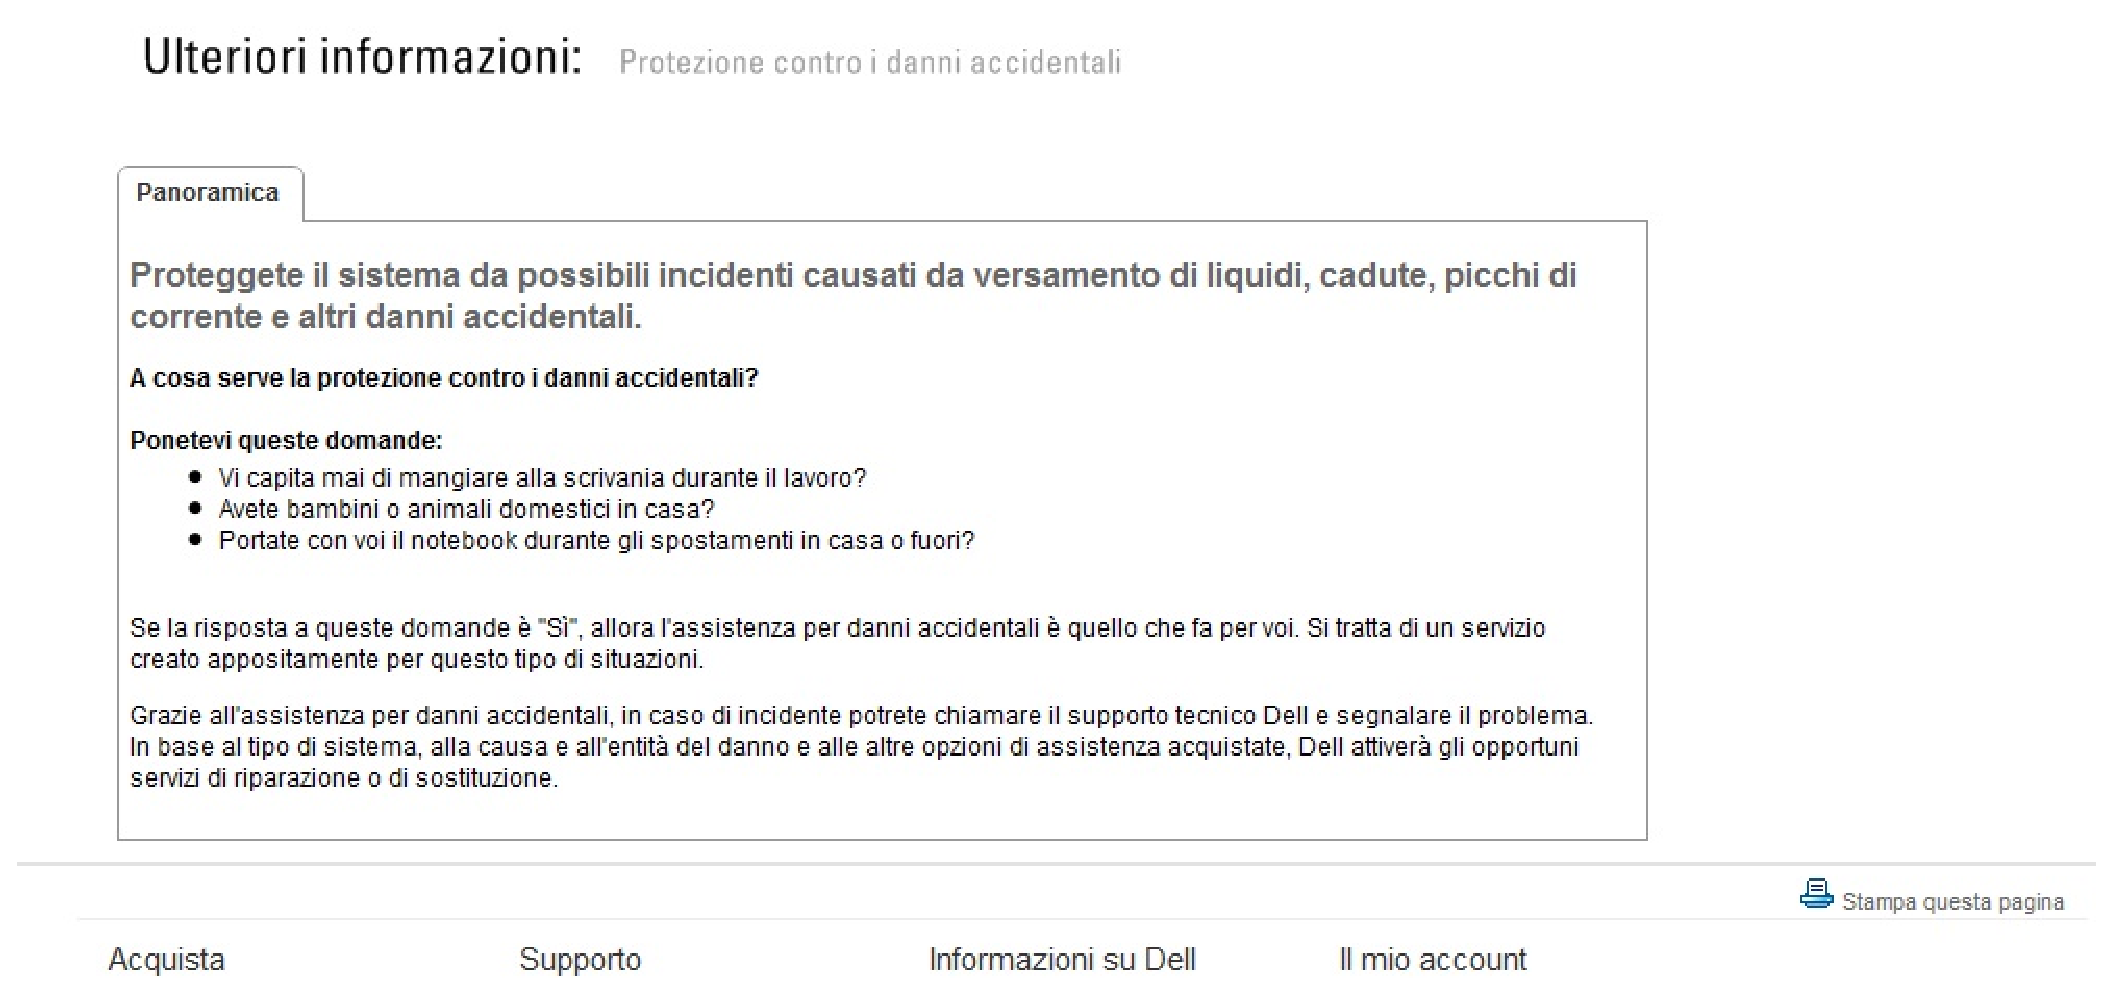
\includegraphics[scale=0.5]{figure/garanzia2.eps}
\caption{La pagina ``esplicativa'' delle informazioni sull'estensione di garanzia}
\label{fig:garanzia}
\end{figure}
\item \underline{Riepilogo componenti scelte}\\
{\bf Descrizione:} Il men� sulla destra contente il riepilogo dei componenti hardware e software acquistati � relegato in una piccola finestra (figura \ref{fig:riepilogo1})\\
{\bf Violazione:} 7 Visualizzare tutte e sole le informazioni necessarie\\
{\bf Criticit�:} 1
\begin{figure}[!h]
\centering
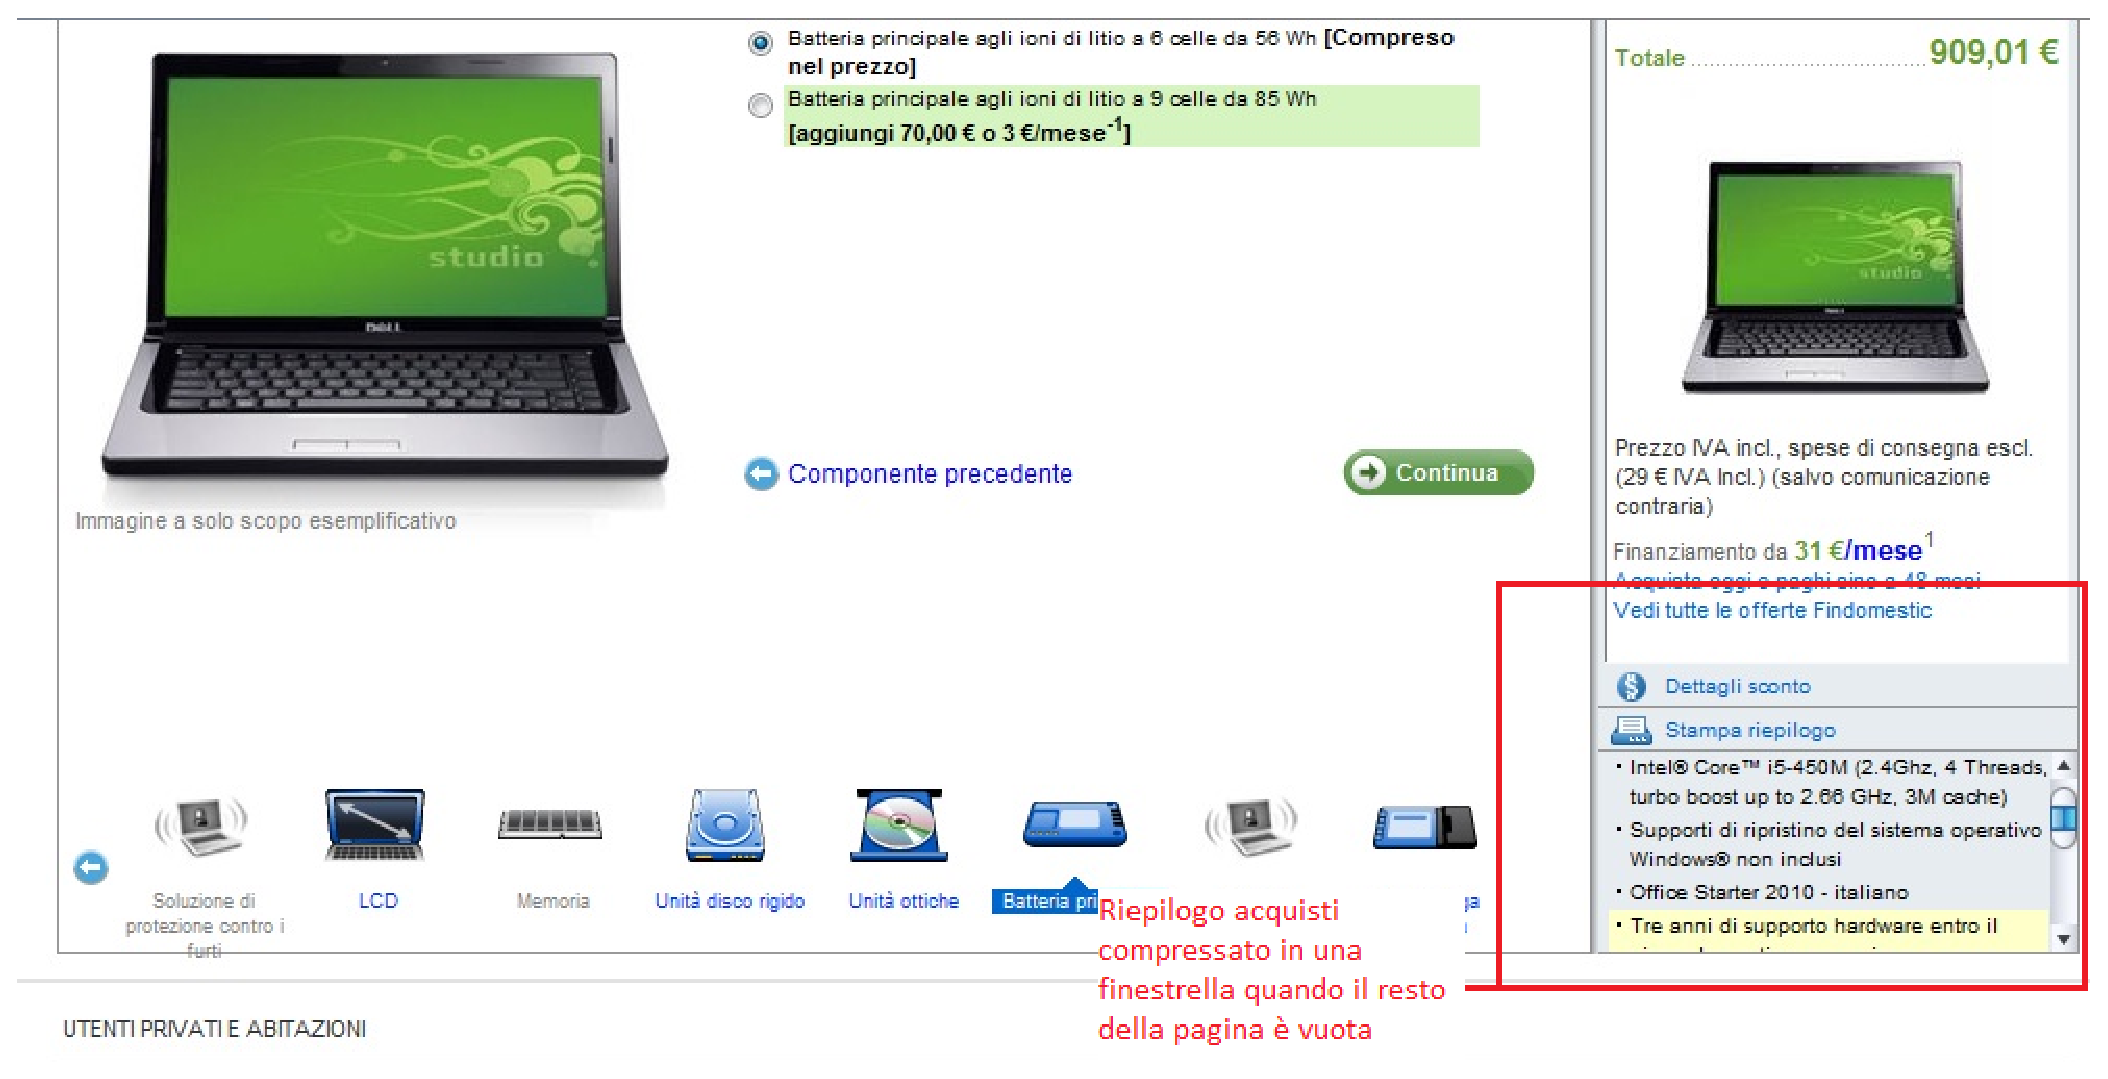
\includegraphics[scale=0.45]{figure/riepilogo1.eps}
\caption{La figura mette in evidenza come sia mal gestito lo spazio della pagina}
\label{fig:riepilogo1}
\end{figure}
\item \underline{Cassa}\\
{\bf Descrizione:} Una volta arrivati nella sezione del pagamento (cassa) non c'� un link di annullamento (figura: \ref{fig:cassa1}).\\
{\bf Violazione:} 3 Controllo dell'utente e libert� (uscite indicate chiaramente)\\
{\bf Criticit�:} 2
\begin{figure}[!h]
\centering
\includegraphics[scale=0.45]{figure/cassa1.eps}
\caption{Nella pagina di cui sopra si ha uno scorcio, non ha alcun link d'annullamento, ma mostra solo un form per i dati dell'utente}
\label{fig:cassa1}
\end{figure}
\item \underline{Incompatibilit� colore}\\
{\bf Descrizione:} Scelta del colore del modello ``studio 15 (649euro)'' segnala una incompatibilit� nella scelta del colore ``black chainlink''\\
{\bf Violazione:} 7 Visualizzazione di tutte e sole le informazioni necessarie, 8 Prevenire gli errori\\
{\bf Criticit�:} 2
\begin{figure}[!h]
\centering
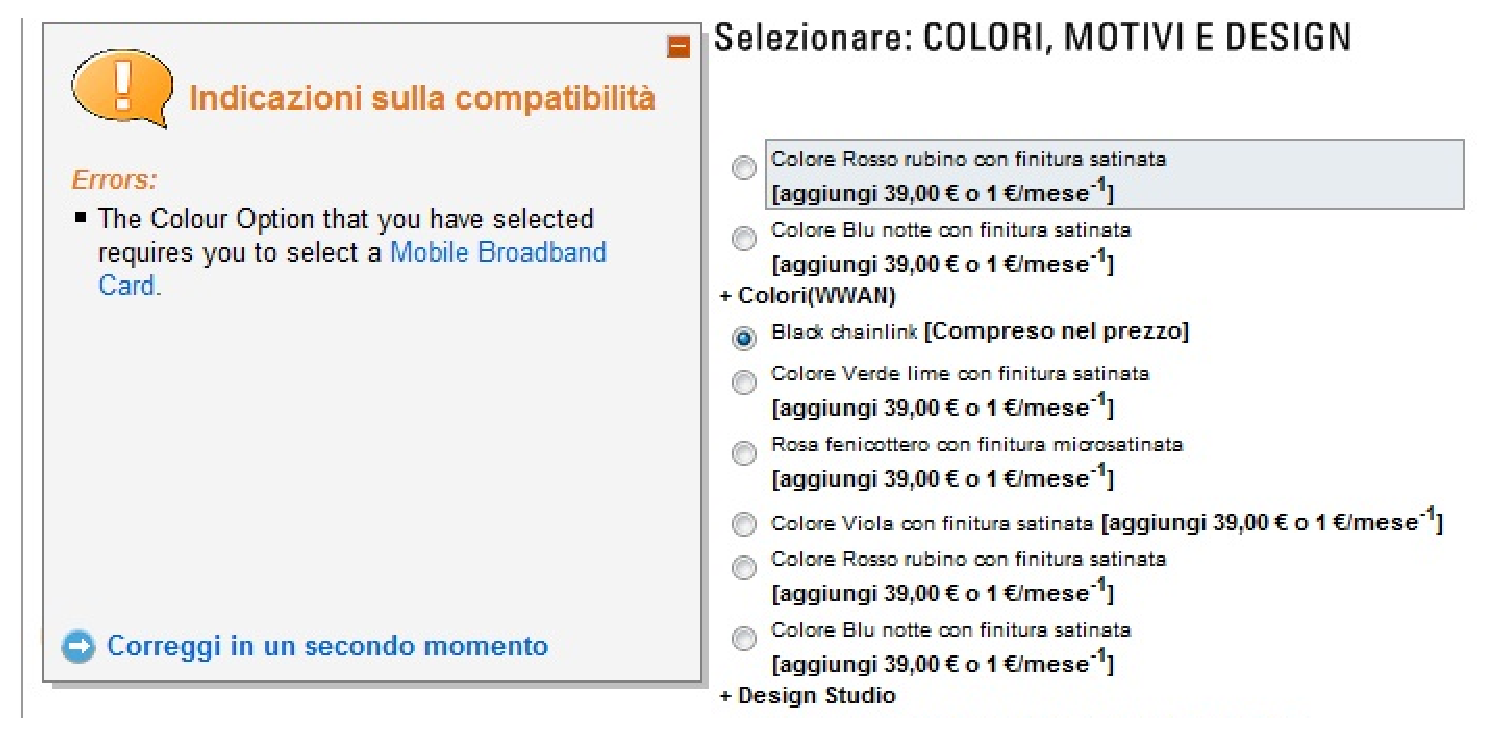
\includegraphics[scale=0.55]{figure/chainlink.eps}
\caption{La figura mostra come un'opzione consentita all'utente produca un errore d'incompatibilit�}
\label{fig:chainlink}
\end{figure}
\item \underline{Mancata traduzione}\\
{\bf Descrizione:}Quando si controlla lo stato del proprio ordine e si inseriscono dati errati, il messaggio d'errore riporta i nomi dei campi in inglese, quando in compilazione essi sono in italiano (figura: \ref{fig:stato_ordine}).\\
{\bf Violazione:} 2 Adeguare il sistema al mondo reale (parlare il linguaggio
dell'utente)\\
{\bf Criticit�:} 1
\begin{figure}[!h]
\centering
\includegraphics[scale=0.65]{figure/stato_ordine.eps}
\caption{La figura mostra in evidenza che alcuni campi non vengono tradotti}
\label{fig:stato_ordine}
\end{figure}
\item \underline{Coupon}\\
{\bf Descrizione:} Errore di inserimento coupon quando scaduto
``Il codice del coupon immesso non � valido. Verificate di aver inserito correttamente il codice e la data di scadenza del coupon''. La dicitura risulta essere fuorviante: la data di scadenza non va inserita, bisogna verificare che il coupon cartaceo sia ancora valido.\\
{\bf Violazione:} 2 Adeguare il sistema al mondo reale (parlare il linguaggio
dell'utente), 8 Prevenire gli errori\\
{\bf Criticit�:} 1
\item \underline{Stato dell'ordine}\\
{\bf Descrizione:} Quando un utente controlla lo stato del proprio ordine, nella sezione ``stato del mio ordine'', il sistema richiede tramite un form i dati dell'ordine da verificare. In tale form � consetito all'utente l'inserimento di caratteri speciali che provocano un errore interno al sistema.\\
{\bf Violazione:} 8 Prevenire gli errori\\
{\bf Criticit�:} 1
\item \underline{Carrello}\\
{\bf Descrizione:} Non sempre possibile tornare allo stato del carrello precedente. Dopo aver cliccato su ``Elimina articolo'' l'articolo in questione viene eliminato senza chiedere alcuna conferma e senza la possibilit� di annullare la scelta.\\
{\bf Violazione:} 3 Controllo dell'utente e libert� (uscite indicate chiaramente), 8 Prevenire gli errori, 9 Permettere all'utente di correggere gli errori e non solo di rilevarli\\
{\bf Criticit�:} 2
\item \underline{Pagina non trovata}\\
{\bf Descrizione:} Per il prodotto ``PowerVault 160T LTO2 (Tape Library)'' selezionando la parte di spiegazione ``cos'� RAID 0 e RAID1'' viene  comunicato che il file di spiegazione non � stato trovato (figure \ref{fig:raid1} e \ref{fig:raid2}).\\
{\bf Violazione principi:} 10 Help e documentazione\\
{\bf Criticit�:} 2
\begin{figure}[!h]
\centering
\includegraphics[scale=0.5]{figure/supporto_raid1.eps}
\caption{La pagina di supporto. In \href{url}{http://www1.euro.dell.com/it/it/abitazioni/laptops\_great}\\
\href{url}{\_deals/fs.aspx?refid=laptops\_great\_deals\&s=dhs\&cs=itdhs1\&\~ck=mn} � evidenziato il link citato nella descrizione del problema}
\label{fig:raid1}
\end{figure}
\\
\begin{figure}[!h]
\centering
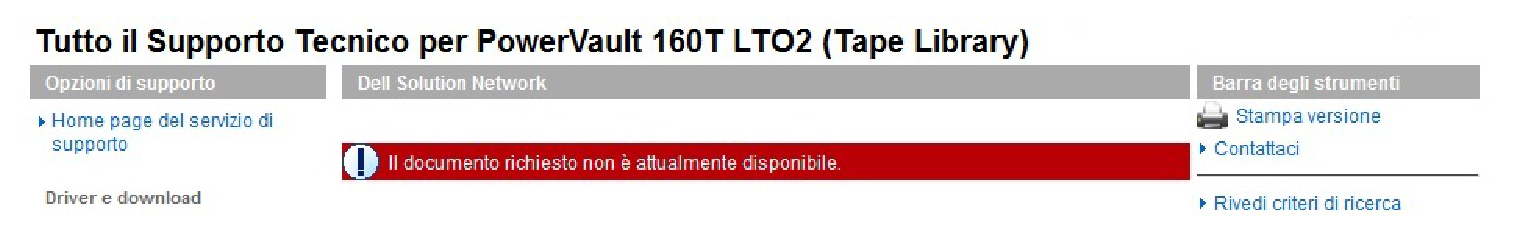
\includegraphics[scale=0.5]{figure/supporto_raid2.eps}
\caption{La pagina di spiegazioni riportante l'errore di documento non trovato}
\label{fig:raid2}
\end{figure}
\item \underline{Privilegi utente}\\
{\bf Descrizione:} Proseguendo nella sezione di supporto e provando ad effettuare delle ricerche all'interno di alcuni prodotti, succede che viene aperta una pagina di errore che comunica all'utente che non ha i privilegi necessari alla visualizzazione della pagina stessa (figura \ref{fig:privilegi}). Inoltre l'avviso di errore � scritto in una lingua di default (inglese) contrariamente a quanto scelto dell'utente\\
{\bf Violazione principi:} 2 Adeguare il sistema al mondo reale (parlare il linguaggio dell'utente), 4 Assicurare consistenza (nell'applicazione, sistema, ambiente), 8 Prevenire gli errori\\
{\bf Criticit�:} 2
\begin{figure}[!h]
\centering
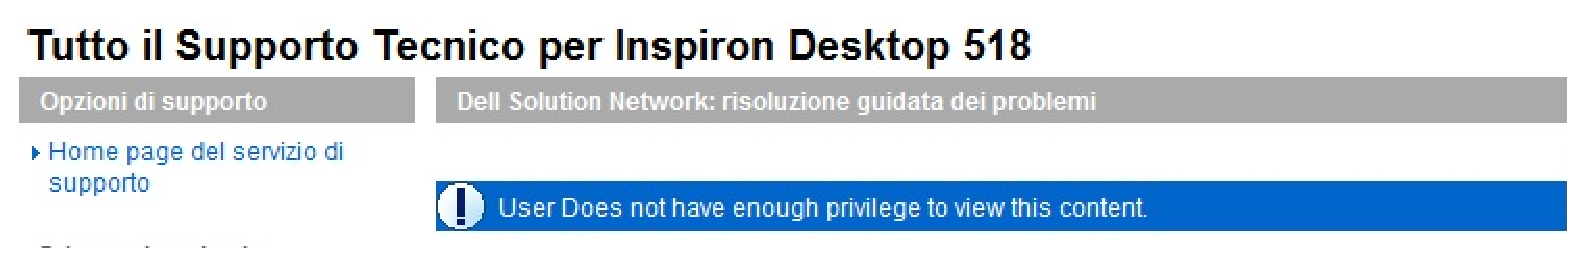
\includegraphics[scale=0.5]{figure/privilegi.eps}
\caption{La pagina di errore per privilegi mancanti}
\label{fig:privilegi}
\end{figure}
\item \underline{Altoparlanti stereo e tv}\\
{\bf Descrizione:} Selezionando ``Altoparlanti stereo e TV'' si ottiene solamente un cavo ``TV Sintonizzatore : Cavo digitale adattatore audio (kit)''. Non pare essere collocato nella categoria adeguata oppure il nome della categoria � inappropriato e poco esplicativo.\\
{\bf Violazione principi:} 4 Assicurare consistenza (nell'applicazione, sistema, ambiente)\\
{\bf Criticit�:} 0
\begin{figure}[!h]
\centering
\includegraphics[scale=0.5]{figure/sintonizzatore.eps}
\caption{Elementi costitutivi della categoria degli ``Altoparlanti stereo e TV''}
\label{fig:sintonizzatore}
\end{figure}
\item \underline{Sezione TVs, Home Theater e audio}\\
{\bf Descrizione:} Selezionando ``TVs, Home Theater e audio'' e cercando i modelli di ``blu-ray'' non si ottiene la pagina voluta, non si ha nemmeno un avviso che non ci sono modelli disponibili \\
{\bf Violazione principi:} 4 Assicurare consistenza (nell'applicazione, sistema, ambiente)\\
{\bf Criticit�:} 1
\item \underline{Riciclaggio Dell}\\
{\bf Descrizione:} Nella sezione privati e cliccando su ``ricicla con Dell'' si accede a una pagina con un form da compilare per poter riciclare. In alto cliccando su ``chiudi'' non succede nulla, pur essendo tale scritta un link attivo.\\
{\bf Violazione principi:} 3 Controllo dell'utente e libert� (uscite indicate chiaramente), 4 Assicurare consistenza (nell'applicazione, sistema, ambiente)\\
{\bf Criticit�:} 2
\item \underline{Riciclaggio Dell}\\
{\bf Descrizione:} Cliccando su uno dei link in azzurro sopra a ``riciclo con Dell'' si apre una nuova finestra di informazioni. Tuttavia � possibile eseguire  il login da tale finestra. Chiudendola e tornando sulla pagina precedente non � segnalato che si � loggati.\\
{\bf Violazione principi:} 1 Far vedere lo stato del sistema (feedback), 4 Assicurare consistenza (nell'applicazione, sistema, ambiente)\\
{\bf Criticit�:} 3
\begin{figure}[!h]
\centering
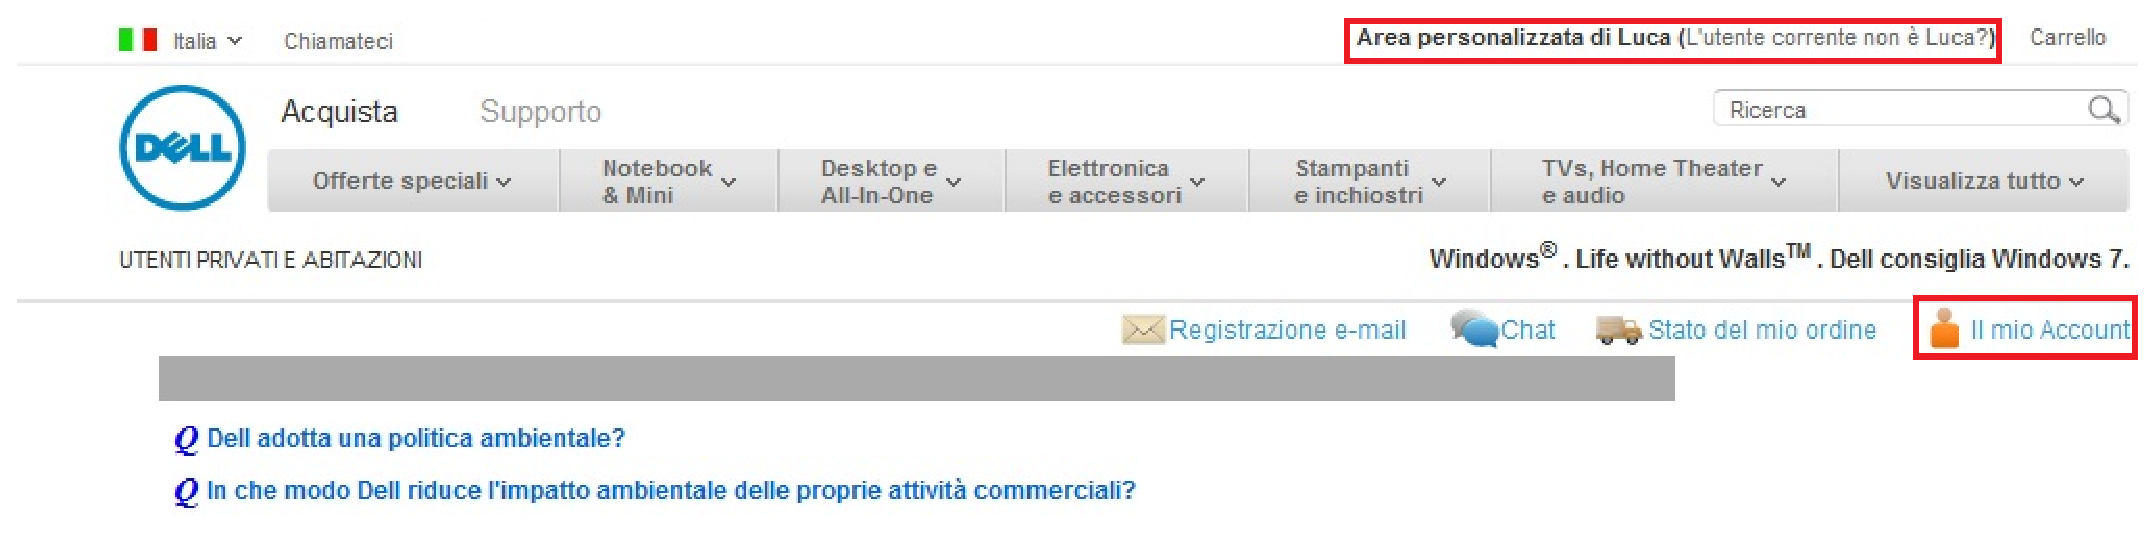
\includegraphics[scale=0.45]{figure/riciclo1.eps}
\caption{Nella nuova finestra si effettua il login, e lo stato dell'utente � modificato come si pu� notare nel riquadro rosso}
\label{fig:riciclo1}
\end{figure}
\begin{figure}[!h]
\centering
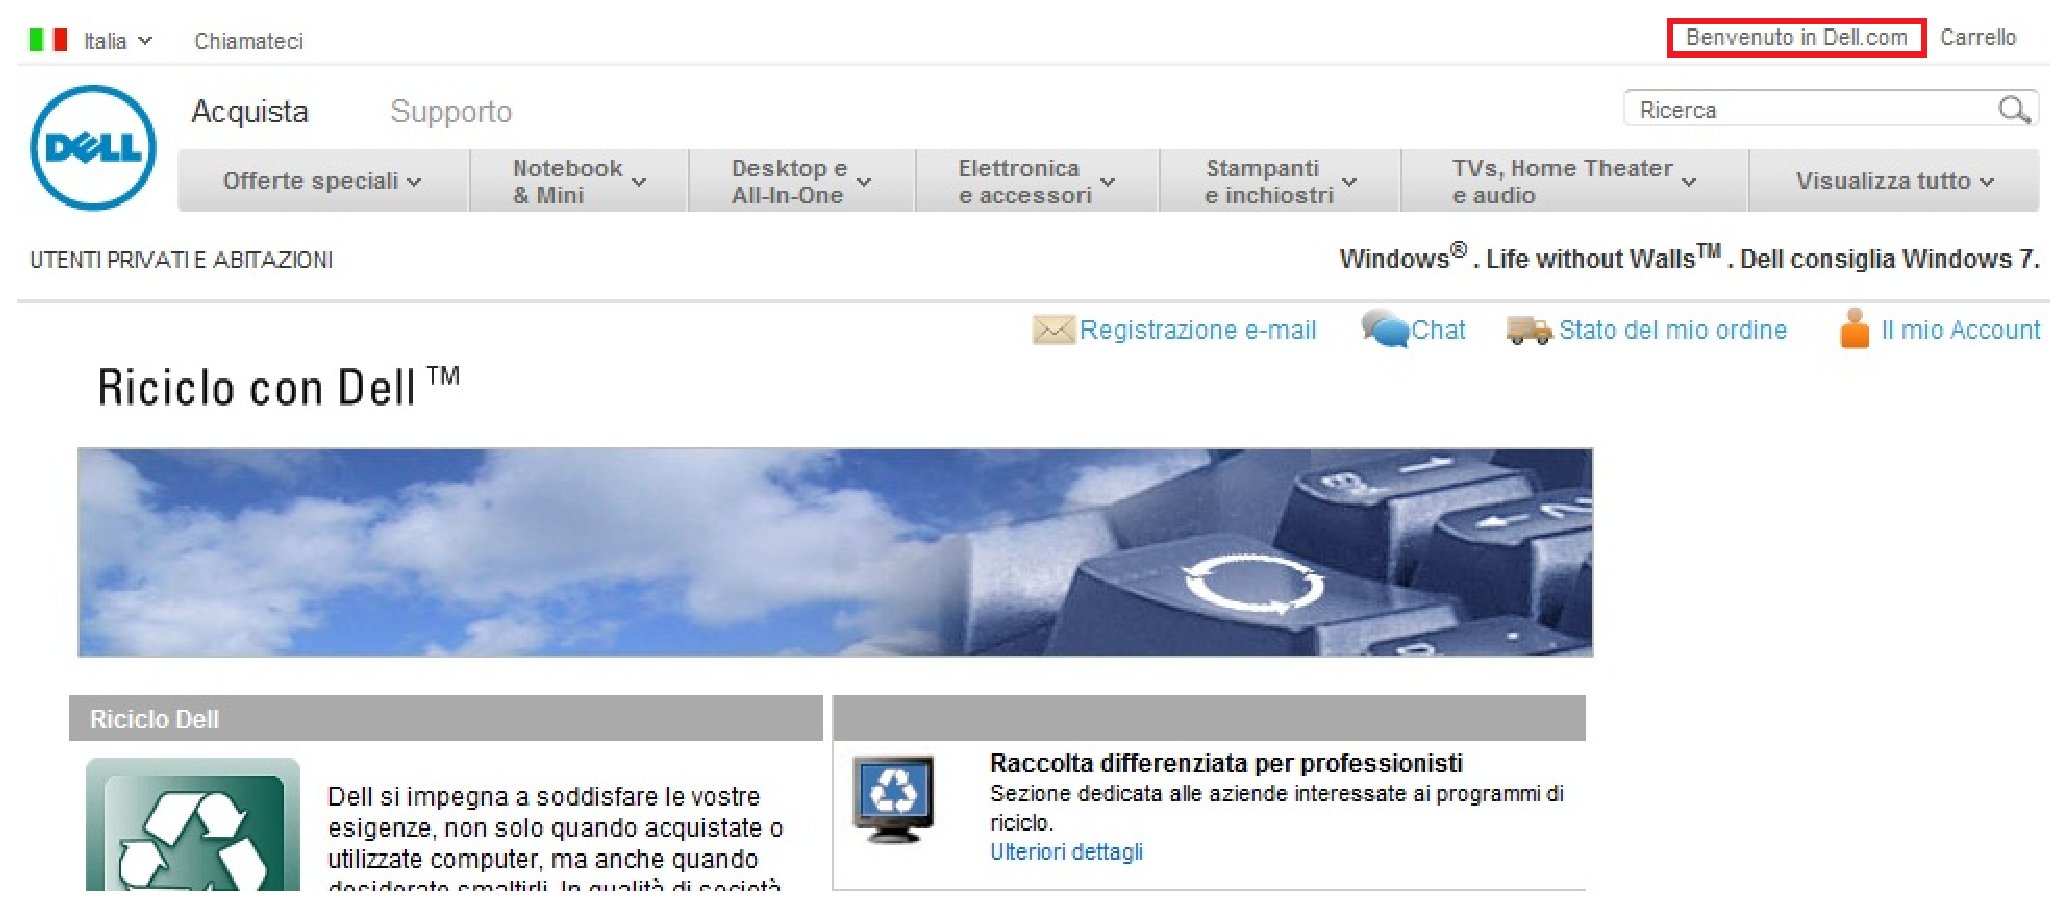
\includegraphics[scale=0.45]{figure/riciclo2.eps}
\caption{Tornando alla pagina si pu� notare in rosso che lo stato dell'utente non � stato aggiornato}
\label{fig:riciclo2}
\end{figure}
\item \underline{Componenti aggiuntivi/essenziali}\\
{\bf Descrizione:} Nella barra di destra sotto ``COMPONENTI AGGIUNTIVI essenziali'' � presente un'immagine che ricorda un messaggio d'errore, quando non dovrebbe. Inoltre i componenti dovrebbero essere ``aggiuntivi'', in quanto opzionali o ``essenziali'', ossia senza i quali il sistema non pu� funzionare; avere entrambe le situazione contemporaneamente � un paradosso.\\
{\bf Violazione principi:} 2 Adeguare il sistema al mondo reale (parlare il linguaggio dell'utente)\\
{\bf Criticit�:} 1
\item \underline{Identificazione prodotto nella sezione ``SUPPORTO''}\\
{\bf Descrizione:} Nella sezione identificazione prodotto per ottenere drivers, nella pagina con la scritta ``identificare il prodotto prima di continuare'' se sceglie il prodotto tramite ``selezione modello'' il redo non � presente\\
{\bf Violazione:} 3 Controllo dell'utente e libert� (uscite indicate chiaramente)\\
{\bf Criticit�:} 1
\item \underline{Opzioni di download}\\
{\bf Descrizione:} Nella sezione di supporto, quando l'utente si trova nella sottosezione ``download option'', la pagina richiede di fornire informazioni riguardanti il proprio sistema operativo ed il proprio browser. Se si sbaglia, in particolare cliccando sul primo bottone di download (che serve solo per windows), tutti i seguenti downloads restano con i parametri inseriti e non � possibile modificarli per ottenere drivers per altri sistemi operativi.\\
{\bf Violazione:} 2 Adeguare il sistema al mondo reale (parlare il linguaggio
dell'utente), 3 Controllo dell'utente e libert� (uscite indicate chiaramente)\\
{\bf Criticit�:} 2
\item \underline{Formato file}\\	
{\bf Descrizione:} Nella descrizione del file ``formato file: disco rigido''. Normalmente nel formato file si indica l'estensione del file o la sua natura (installatore o altro)\\
{\bf Violazione:} 2 Adeguare il sistema al mondo reale (parlare il linguaggio
dell'utente), 7 Visualizzare tutte e sole le informazioni necessarie (figura: \ref{fig:drivers})\\
{\bf Criticit�:} 1
\begin{figure}[!h]
\centering
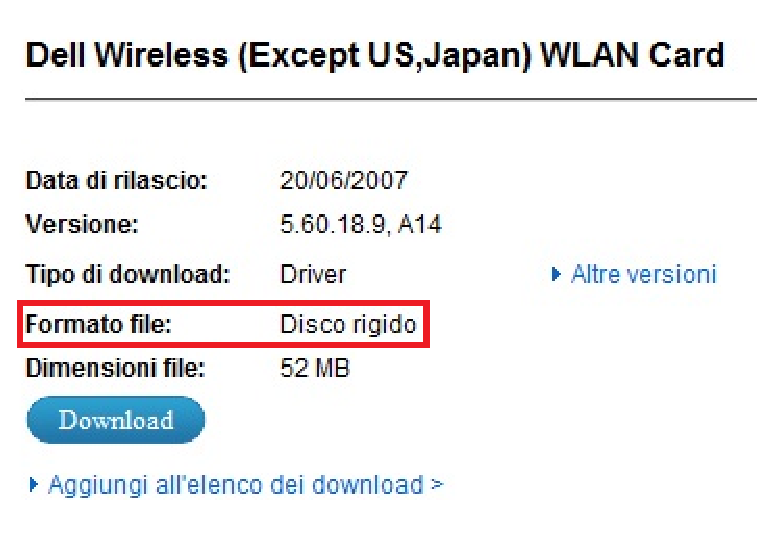
\includegraphics[scale=0.7]{figure/driver.eps}
\caption{Errore di dicitura: solitamente per ``tipo file'' non si esprime il supporto, ma l'estensione}
\label{fig:drivers}
\end{figure}
\item \underline{Download manuali}\\
{\bf Descrizione:} Nella sezione di download dei manuali c'� una scritta che sembra un link ma � solo un'impressione: il click su di esso non produce alcun effetto (figura: \ref{fig:manuali1})\\
{\bf Violazione:} 4 Assicurare consistenza (nell'applicazione, sistema, ambiente)\\
{\bf Criticit�:} 1
\begin{figure}[!h]
\centering
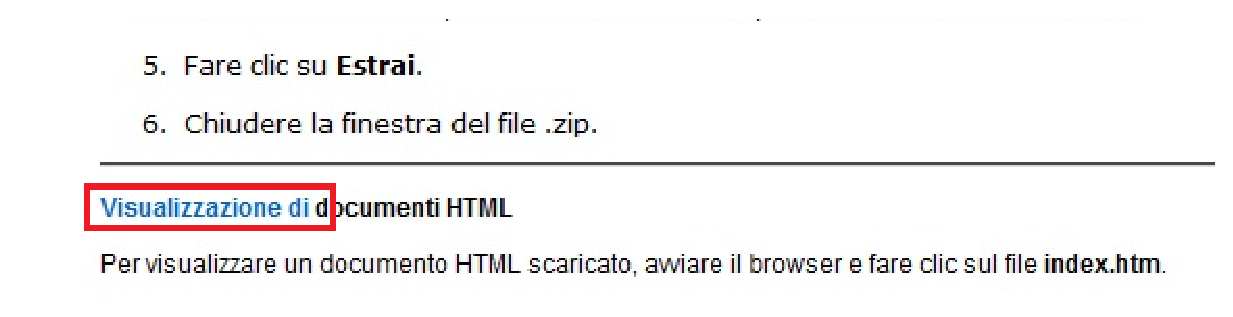
\includegraphics[scale=0.6]{figure/manuali1.eps}
\caption{Evidenziata in rosso la scritta che ha la stessa colorazione di un link}
\label{fig:manuali1}
\end{figure}
\begin{figure}[!h]
\centering
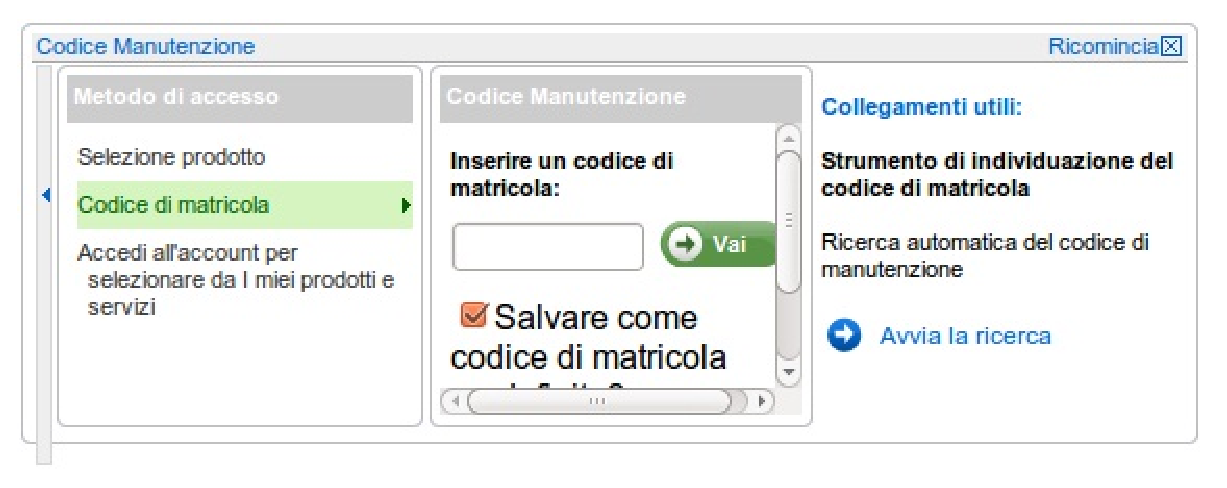
\includegraphics[scale=0.75]{figure/manutenzione.eps}
\caption{Si nota come la tabella sia formattata in modo troppo piccolo, tuttavia si ricorre allo scroll per visualizzare il resto del contenuto}
\label{fig:manutenzione}
\end{figure}
\item \underline{Identificazione prodotto}\\ 
{\bf Descrizione:} Lo schema per identificare un prodotto � una tabellina formattata in modo troppo piccolo. Il resto della pagina � completamente vuoto e di conseguenza non si da risalto al link di aiuto per trovare il codice matricola (figura \ref{fig:manutenzione})\\
{\bf Violazione:} 7 Visualizzare tutte e sole le informazioni necessarie\\
{\bf Criticit�:} 1
\item \underline{Cartina geografica del mondo}\\
{\bf Descrizione:} Nella sezione ``Opportunit� di lavoro'' viene mostrata la cartina mondiale. Posizionando anche il cursore sulla cartina nella zona asiatica viene comunque scritto ``Europe, Middle east, Africa''\\
{\bf Violazione:} 2 Adeguare il sistema al mondo reale (parlare il linguaggio
dell'utente), 7 Visualizzare tutte e sole le informazioni necessarie\\
{\bf Criticit�:} 0
\begin{figure}[!h]
\centering
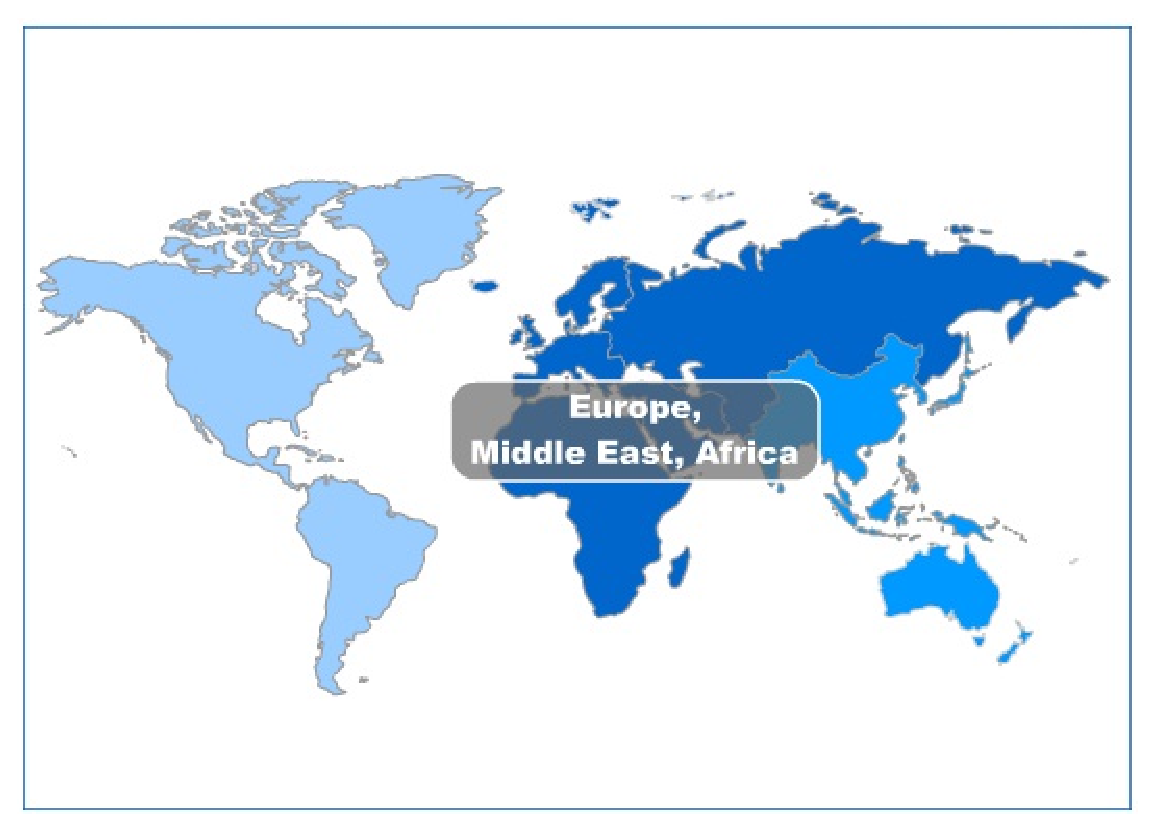
\includegraphics[scale=0.65]{figure/cartina.eps}
\caption{La cartina con evidenziata l'area asiatica che per� viene riconosciut� come ``Europa, Medio Oriente, Africa''}
\label{fig:cartina}
\end{figure}
\item \underline{Banner pubblicitario}\\
{\bf Descrizione:} Talvolta all'interno della pagina ''LINKROSSO APPUNTI'' compare un banner di help che si posiziona sopra al contenuto della pagina, coprendo le informazioni sottostanti, restando in una posizione fissa rispetto alla finestra del browser.\\
{\bf Violazione:} 7 Visualizzare tutte e sole le informazioni necessarie\\
{\bf Criticit�:} 1
\item \underline{Mancata traduzione}\\
{\bf Descrizione:} Quando si passa col cursore sulla scritta carrello in alto a destra  durante il caricamento viene riportata la scritta ``Loading'' e quando c'� qualcosa nel carrello a indicare il numero di pezzi scelti c'� ``Quantity''.\\
{\bf Violazione:} 2 Adeguare il sistema al mondo reale (parlare
\input{section2_5.tex}


\cleardoublepage
\chapter{Esperimento con gli utenti}
Successivamente all'analisi euristica abbiamo deciso di effettuare l'esperimento con gli utenti. Questa fase del lavoro � stata impiegata per poter avere un maggiore riscontro rispetto ad un analisi effettuata dai soli valutatori, in questo modo si � potuto vedere quali sono state le effettive problematiche incontrate dagli utenti durante la navigazione del sito web.

\subsection*{Scelta degli utenti}
Innanzitutto abbiamo deciso quale dovesse essere il campione di utenti al quale sottoporre il test in questione. Siccome la sezione del sito Dell riguardante i privati pu� essere ,in genere, acceduta da utenti di tipo piuttosto eterogeneo si � scelto un campione di utenti con differenti capacit�, per cercare di rispecchiare al meglio le tipologie di utenti che accedono al sito.
Gli utenti sono stati suddivisi in due categorie:
\begin{itemize}
\item utenti esperti, ossia con buone conoscenze informatiche e abituato a navigare il web per diversi usi
\item utenti non esperti, ossia con poche conoscenze informatiche
\end{itemize}
Abbiamo quindi deciso di effettuare il test su 20 utenti per esaminatore, di cui la met� esperti e l'altra con discrete conoscenze informatiche. 
Pi� nel dettaglio abbiamo stabilito che gli utenti ``esperti'' avessero precedenti esperienze nell'ambito di acquisti on-line e che siano abituati a navigare il web per leggere la posta o per cercare informazioni. Gli utenti che invece non rispettano questi requisiti ricadono nella classe da noi definito come utenti ``non esperti'', abbiamo giudicato che per poter svolgere il test essi dovessero avere conoscenze informatiche di base, ossia che sappiano accedere ad un sito web dicendo loro l'indirizzo a cui accedere ed abbiano una, seppur minima, capacit� di navigarlo.\\
Questa divisione � stata effettuata per cercare di valutare se conoscenze pregresse aiutassero in maniera decisiva a sfruttare gli acceleratori del sito o se restassero prevalentemente inutilizzati anche per essi.\\
\subsection*{Criteri di definizione del test}
Per quanto riguarda il test vero e proprio, come prima cosa abbiamo cercato di immaginare uno scenario di utilizzo tipico, che coprisse le attivit� che presumibilmente un utente svolge quando utilizza il sito Dell. In seguito a ci� abbiamo stabilito di quali parti dovesse essere formato. L'idea � che il sito venga impiegato per effettuare l'acquisto di un computer e per attivit� correlate come cercare driver e software accessorio.
Come risultato di queste analisi abbiamo quindi deciso di prendere in considerazione uno scenario nel quale l'utente accede al sito Dell per la prima volta (importante) e, nell'ordine, si registra, confronta alcuni computer, ne compra uno (tenendo in considerazione che nel nostro caso l'acquisto non avviene effettivamente) ed effettua il logout. Oltre a queste operazioni ne sono state inserite altre non strettamente inerenti all'acquisto di una macchina, per osservare come l'utente si destreggiasse nel passare dall'area acquisto a quella di supporto.

\subsection*{Fase preliminare}
Ai fini di ottenere dei risultati quanto pi� veritieri possibile abbiamo cercato di mettere l'utente a suo agio, affinch� l'agitazione non influisse sugli esiti dei test. Per cercare di mettere l'utente nelle condizioni ottimali di fruizione del sito Dell, gli abbiamo lasciato libert� riguardo la scelta della piattaforma sulla quale eseguire il test. Non sono quindi stati posti vincoli sulla natura del calcolatore, ne del sistema operativo utilizzato, ne del browser con il quale il sito � stato navigato. Agli utenti � stato inoltre premesso di impiegare il proprio calcolatore, in modo che fossero nelle condizioni in cui si trova ad interagire solitamente con i siti web.  Nei casi in cui ci� non � stato possibile si � optato per macchine con le quali l'utente avesse familiarit�, affinch� i risultati del test non fossero falsati da quest'ultima.\\
Infine abbiamo verificato che le connessioni ad internet fossero adeguate ad una navigazione del sito senza introdurre ritardi nel passaggio da una pagina a quella successiva.
Prima di iniziare la prova abbiamo spiegato ad ogni utente che l'oggetto della valutazione era il sito Dell e non le prestazioni da loro ottenute nello svolgere i task, o un eventuale fallimento nel portarlo a termine. � stato inoltre spiegato che il test sarebbe dovuto essere svolto senza fretta alcuna, procedendo alla velocit� che pi� gli si confaceva, e che procedesse come se volesse effettivamente svolgere i task di propria iniziativa.\\
\newline
Prima dell'esecuzione vera e propria abbiamo anche verificato che l'utente conoscesse la nomenclatura utilizzata per esprimere i vari task, e comprendesse quale fosse l'obiettivo di ognuno, chiarendo quindi gli eventuali dubbi.

\section{Task}
I vari task sono stati scelti in modo che l'utente avesse ben chiaro quale fosse l'obiettivo da raggiungere. Inoltre ognuno di essi doveva rispettare alcuni criteri:
\begin{itemize}
\item Il task deve poter essere svolto a partire da una qualsiasi pagina del sito
\item l'obiettivo del task deve essere chiaro all'utente
\item non devono essere presenti vicoli ciechi dai quali l'utente non possa pi� tornare in dietro
\end{itemize}
Oltre a questo alcuni task sono stati scelti per poter essere svolti in modi differenti. Per ogni task � stata decisa la massima durata entro la quale dovesse essere svolto, senza tuttavia comunicarla agli utenti, in modo da non metterli sotto pressione. Qualora il tempo massimo stabilito dai valutatori venisse sforato il task viene considerato fallito, stessa cosa anche nei casi in cui il task � stato svolto in modo incompleto, o non svolto del tutto.\\
\newline
Il primo task non � significativo dal punto di vista dell'esaminatore, � stato inserito solamente per mettere l'utente a proprio agio.\\
Elenco dei task:
\begin{enumerate}
\item {\it Accesso al sito www.dell.it}, compito elementare, non utile ai fini della valutazione
\item  {\it Ricerca prodotto}, visualizzare i prodotti Blu-ray. Task semplice.\\
Quando il task si ritiene concluso: nel momento in cui l'utente accede alla pagina riguardante i prodotti Blu-ray.\\
Tempo massimo previsto:2 minuti
\item {\it Confronto notebook}, accedere alla pagina di confronto dei due notebook ``{\bf Inspiron 15R}'' e ``{\bf Inspiron M501R}''. Test di media difficolt� richiede di accedere alla pagina di confronto, e poi di selezionare i due notebook e confermare.\\
Quando il task si ritiene concluso: quando l'utente visualizza la pagina di confronto tra i due notebook.\\
Tempo massimo previsto: 3min.
\item {\it Registrazione di un nuovo account}, creare un nuovo account utente. Task di media difficolt� prevede il raggiungimento della pagina di registrazione e la compilazione di un form.\\ 
Quando il task si ritiene concluso: quando l'utente ha registrato un nuovo utente.\\
Tempo massimo previsto: 4 minuti
\item {\it Ricerca drivers}, visualizzare tutti i driver disponibili per il laptop modello ``{\bf Studio XPS Laptop 1645}''. Task di difficolt� medio alta, composto da diverse fasi: bisogna innanzitutto entrare nell'area di supporto, passare alla sottosezione drivers, identificare il modello corretto e scegliere di mostrare il software disponibile per il modello in questione.\\
Quando il task si ritiene concluso: quando l'utente visualizza i drivers per il suddetto Laptop.\\
Tempo massimo previsto: 4 minuti.
\item {\it Aggiunta al carrello di un computer}, personalizzare e mettere nel carrello un desktop ``Inspiron M501R'' con le seguenti caratteristiche:
\begin{itemize}
\item Processore AMD Phenom II Triple-Core N850 
\item Microsoft Office 2007 Home and Student
\end{itemize}
Task di difficolt� medio alta, dovuta al numero di step da percorrere per portarlo a termine.\\
Quando il task si ritiene concluso: nel momento in cui un computer viene aggiunto al carrello, nel caso in cui il computer non corrisponda alle caratteristiche sopra definite il task � considerato fallito.\\
Tempo massimo previsto: 5 minuti.
\item {\it Logout}, effetuare il logout senza chiudere il browser. Task rapido, ma non banale in quanto in molte pagine non � presente il link per il logout e pu� inoltre avere un aspetto diverso a seconda della pagina nella quale ci si trova.\\ 
Quando il task si ritiene concluso: nel momento in cui si � effettuato il logout.\\
Tempo massimo previsto: 1 minuto.
\item {\it Aggiunta al carrello di un secondo computer}, di tipo ``{\bf Dell Studio 15''} personalizzato con le seguenti caratteristiche:
\begin{itemize}
\item Intel core i3 Windows 7 Home Premiom;
\item Colore Blu ;
\item Microsoft Office 2010 Professional;
\item Supporti di ripristino del sistema operativo: DVD di risorse di Windows 7 Home Premium;
\item Quattro anni di supporto hardware entro il giorno lavorativo successivo, con protezione contro danni accidentali;
\item Backup Online 50Gb;
\item Valigetta;
\item Unit� di storage esterna di almeno 250Gb;
\item Alimentatore di riserva;
\end{itemize}
Task di difficolt� medio alta, dovuta prevalentemente all'elevata sequenza di passaggi che l'utente deve svolgere per arrivare a termine e al numero di caratteristiche da configurare correttamente: entrare nella sezione notebook, scegliere il calcolatore, configurarlo in vari passi, senza omettere nessuna caratteristica.\\
Quando il task si ritiene concluso: nel momento in cui un computer viene aggiunto al carrello, nel caso in cui il computer non corrisponda alle caratteristiche sopra definite il task � considerato fallito.\\
Tempo massimo previsto: 7 minuti.
\item {\it Salvataggio del nuovo portatile nel proprio account}\\ 
Task di media difficolt�, bisogna salvare la configurazione in modo corretto, essendo possibile effettuare il log-in senza salvarla perdendo tutti i dati della configurazione.\\
Quando il task � considerato concluso: quando la configurazione del portatile  Dell Studio15 viene salvata all'interno dell'account creato in precedenza.\\
Tempo massimo previsto 3 minuti.
\item {\bf Eliminazione prodotto}, ``{\bf Inspiron M501R}'' dal carrello,  cancellare il prodotto inserito in precedenza nel carrello. Task semplice, pu� essere eseguito tramite il baloon che appare passando su ``carrello'' in alto a destra, oppure dall'apposita sezione. Task di bassa difficolt�.\\
Quando il task si ritiene concluso: nel momento in cui il computer aggiunto al carrello al punto precedente viene rimosso dal carrello (nel caso in cui il punto precedente non fosse stato portato a termine il valutatore deve provvedere ad aggiungere al carrello un computer prima dell'inizio di questo punto).\\
Tempo massimo previsto: 1 minuto.

\end{enumerate}

\section{Documento presentato agli utenti}
Come detto nei precedenti paragrafi il documento presentato agli utenti � stato scritto in modo da mettere l'utente quanto pi� a suo agio possibile. Per perseguire questo fine abbiamo deciso di scrivere il documento in maniera informale, tenendo conto anche del fatto che gli utenti sono persone conosciute dai valutatori, sarebbe stato perci� una forzatura rivolgersi ad essi in maniera formale.\\
\newline
Di seguito � riportato il documento sottoposto agli utenti:\\
\newline
QUI C'� UN PEZZO VUOTO NELLA PARTE 3 DI RIZZARDI CHE NON SO COSA CI VADA\\
\newline
Esperimento - Valutazione sito www.dell.it\\
\newline
Innanzitutto ti ringraziamo per la partecipazione.\\
\newline
Lo scopo di questo test � quello di valutare l'usabilit� del sito www.dell.it  e non giudicare le tue abilit� nel portare a termine i vari compiti.\\
Affronta i vari quesiti con calma, senza preoccuparti di portare a termine ogni compito.\\
\newline
Istruzioni per lo svolgimento:
\begin{itemize}
\item cerca di svolgere i compiti riportati di seguito uno alla volta, nell'ordine in cui sono elencati;
\item quando giungi al termine di ogni singolo compito indica il grado di difficolt� che hai incontrato durante lo svolgimento;
\item quando hai terminato ogni singolo compito avverti il valutatore;
\item prima dell'inizio dei vari compiti puoi chiedere chiarimenti, ma non suggerimenti su come portarlo a termine.
\end{itemize}
Ti ricordiamo ancora una volta che lo scopo di questo test � valutare il sito Dell, non le tue capacit�. Ora puoi iniziare a leggere i quesiti, se hai dei dubbi sentiti libero di chiedere chiarimenti al valutatore.\\
\begin{enumerate}
\item {\it Accedi al sito www.dell.it};\\
Indica la difficolt� di questo compito:\\
-banale \hspace{1cm} -facile \hspace{1cm} -medio \hspace{1cm} -impegnativo \hspace{1cm} -difficile 
\item {\it Visualizza i prodotti Blu-Ray};\\
Indica la difficolt� di questo compito:\\
-banale \hspace{1cm} -facile \hspace{1cm} -medio \hspace{1cm} -impegnativo \hspace{1cm} -difficile 
\item 1. Confronta i due notebook ``Inspiron 15R'' e ``Inspiron M501R'';\\
Indica la difficolt� di questo compito:\\
-banale \hspace{1cm} -facile \hspace{1cm} -medio \hspace{1cm} -impegnativo \hspace{1cm} -difficile
\item {\it Registra un nuovo account};\\
Indica la difficolt� di questo compito:\\
-banale \hspace{1cm} -facile \hspace{1cm} -medio \hspace{1cm} -impegnativo \hspace{1cm} -difficile 
\item {\it Trova i drivers disponibili per il laptop ``Studio XPS Laptop 1645''};\\
Indica la difficolt� di questo compito:\\
-banale \hspace{1cm} -facile \hspace{1cm} -medio \hspace{1cm} -impegnativo \hspace{1cm} -difficile
\item {\it Aggiunta al carrello del computer}, ``Inspiron M501R'' con le seguenti caratteristiche:
\begin{itemize}
\item Processore AMD Phenom II Triple-Core N850 
\item Microsoft Office 2007 Home and Student
\end{itemize}
Indica la difficolt� di questo compito:\\
-banale \hspace{1cm} -facile \hspace{1cm} -medio \hspace{1cm} -impegnativo \hspace{1cm} -difficile
\item {\it Effetuare il logout senza chiudere il browser};\\
Indica la difficolt� di questo compito:\\
-banale \hspace{1cm} -facile \hspace{1cm} -medio \hspace{1cm} -impegnativo \hspace{1cm} -difficile
\item {\it Aggiungi al carrello un computer, di tipo ``Dell Studio 15'' con le seguenti caratteristiche}:
\begin{itemize}
\item Intel core i3 Windows 7 Home Premiom;
\item Colore Blu ;
\item Microsoft Office 2010 Professional;
\item Supporti di ripristino del sistema operativo: DVD di risorse di Windows 7 Home Premium;
\item Quattro anni di supporto hardware entro il giorno lavorativo successivo, con protezione contro danni accidentali;
\item Backup Online 50Gb;
\item Valigetta;
\item Unit� di storage esterna di almeno 250Gb;
\item Alimentatore di riserva;
\end{itemize}
Indica la difficolt� di questo compito:\\
-banale \hspace{1cm} -facile \hspace{1cm} -medio \hspace{1cm} -impegnativo \hspace{1cm} -difficile
\item {\it Salva il portatile appena aggiunto al carrello nell'account che hai creato prima};\\
Indica la difficolt� di questo compito:\\
-banale \hspace{1cm} -facile \hspace{1cm} -medio \hspace{1cm} -impegnativo \hspace{1cm} -difficile
\item {\it Elimina il prodotto ``Inspiron M501R'' dal carrello}.
Indica la difficolt� di questo compito:\\
-banale \hspace{1cm} -facile \hspace{1cm} -medio \hspace{1cm} -impegnativo \hspace{1cm} -difficile
\end{enumerate}

\section{Debriefing ed esiti dell'esperimento}
Lo scopo di questo paragrafo � quello di analizzare i dati raccolti dall'esperimento con l'utente ed esplicitarne gli esiti. Nelle varie analisi i dati verranno mostrati suddivisi per categoria di utente (che ricordiamo aver definito come ``esperti'' e ``non esperti'') in un unico grafico, per mostrare meglio le differenze nei tempi in cui vengono portati a termine i compiti, a seconda delle categorie di utenti.
\subsection*{Giudizio espresso dall'utente}
Grafico riguardante la valutazione degli utenti in riferimento ai vari task, nel seguente grafico (figura:\ref{fig:grafico_difficolta}) sono mostrate le valutazioni medie di difficolt�, utilizzando i seguenti valori come pesi: banale 0; facile 1; medio 2; impegnativo 3; difficile 4.
\begin{figure}[!h]
\centering
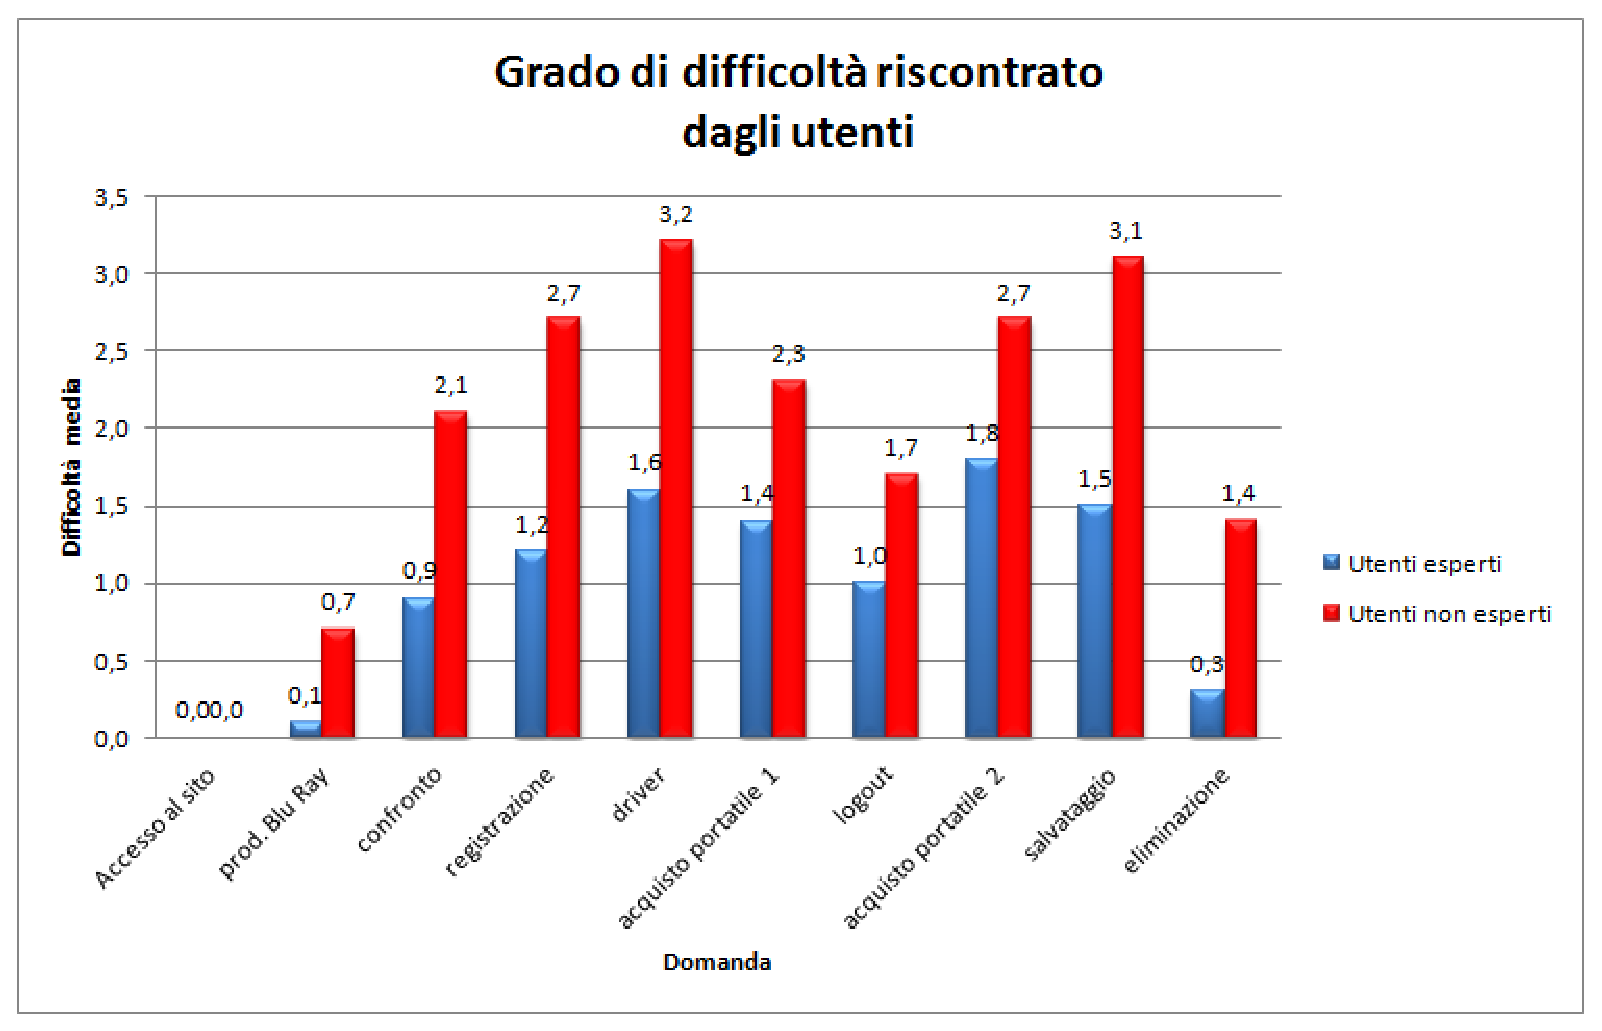
\includegraphics[angle=90,scale=0.75]{figure/grafico_difficolta.eps}
\caption{Grafico media delle difficolt� dei due gruppi d'utenti esaminati}
\label{fig:grafico_difficolta}
\end{figure}
Come evidenziato dal grafico gli utenti esperti considerano i compiti a loro assegnato notevolmente pi� semplici dei loro corrispettivi non esperti. In particolare si evidenzia che la fase di registrazione e di salvataggio della configurazione del secondo portatile risultano avere una valutazione di difficolt� pi� che doppia. Si nota inoltre che alcuni compiti che dovrebbero risultare semplici in realt� non siano tali, come ad esempio la registrazione ed il salvataggio delle proprie impostazioni. Inoltre alcuni utenti hanno valutato la difficolt� di compiti da loro eseguiti fuori tempo massimo o in maniera errata come facile o media.

\subsection*{Valutazione di tempi ed errori}
Esponiamo ora i dati oggettivi raccolti dai due valutatori ossia il tempo impiegato per risolvere i vari task, e gli errori riscontrati per ogni singolo task. Nei seguenti diagrammi si � deciso di mantenere i dati di utenti esperti e non esperti separati, come abbiamo fatto nel paragrafo precedente.


\begin{figure}[!h]
\centering
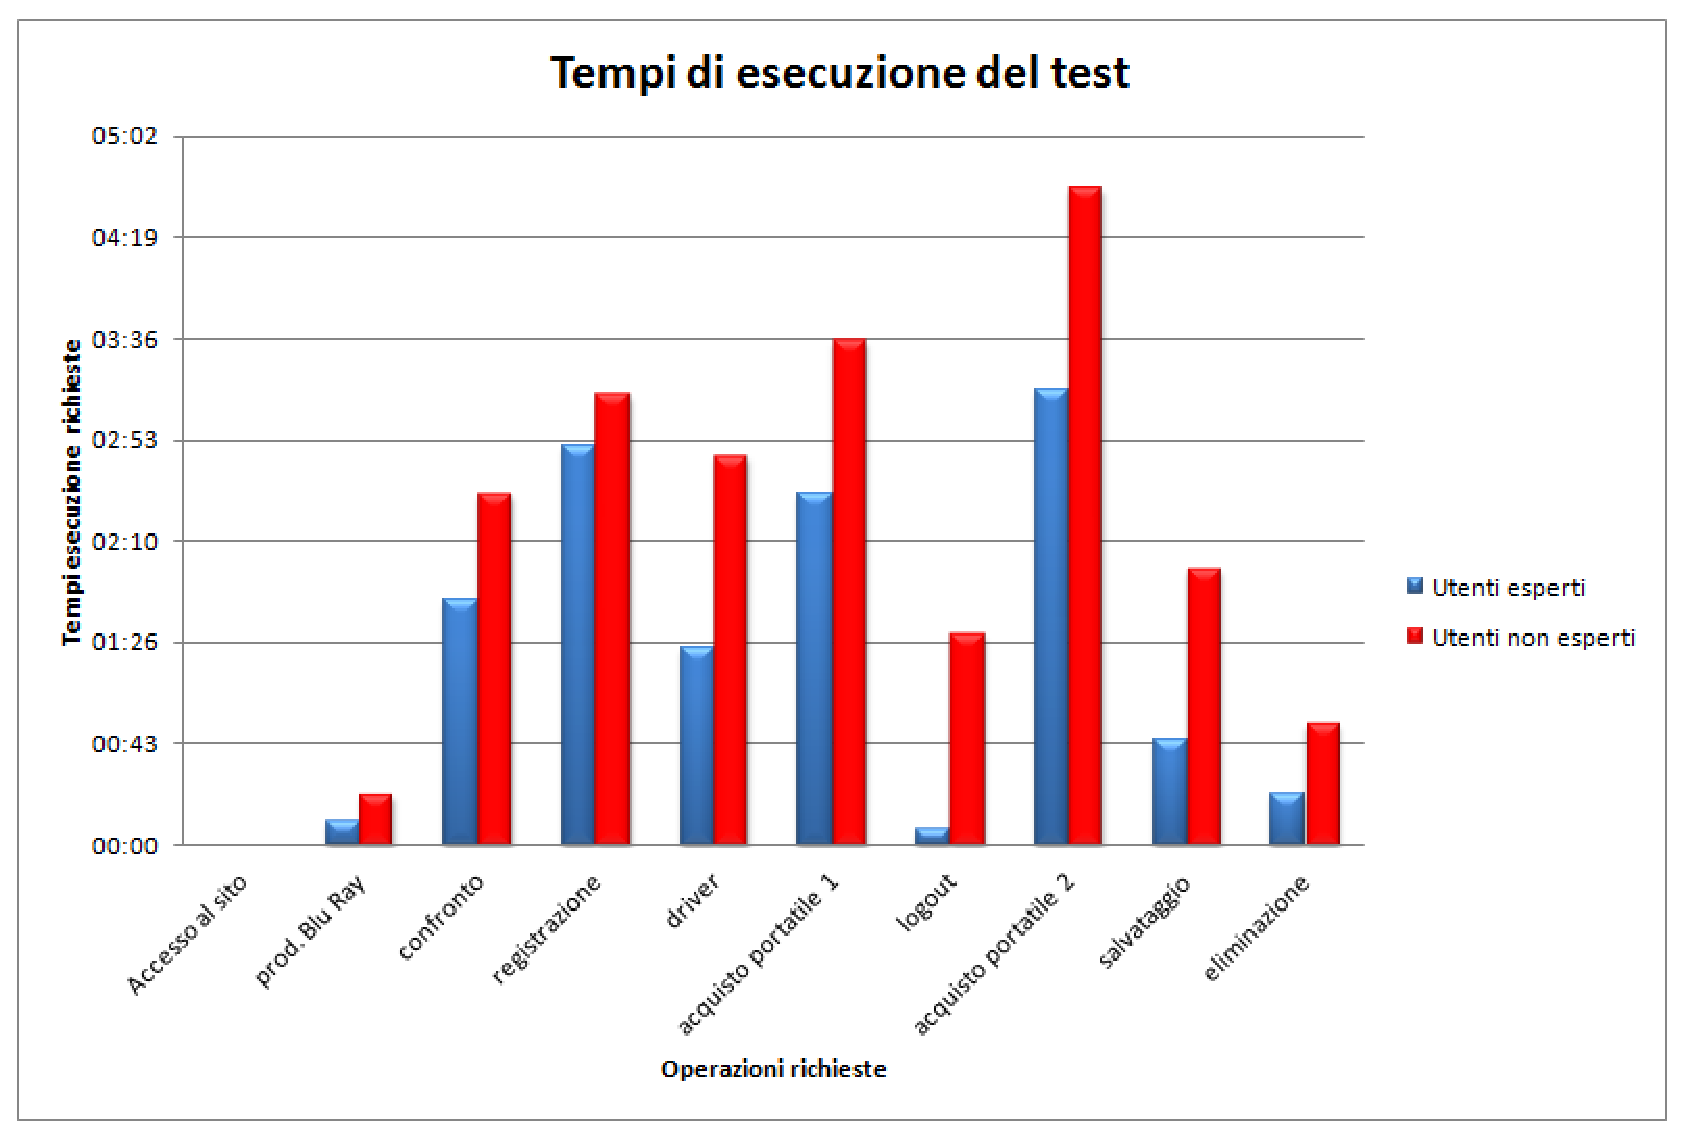
\includegraphics[angle=90, scale=0.75]{figure/grafico_tempi_esecuzione.eps}
\caption{Grafico riportante i tempi di esecuzione delle varie domande del test}
\label{fig:tempi_esecuzione_test}
\end{figure}

Dopo il grafico riguardante i tempi medi passiamo a vedere quello riguardante la quantit� di errori:

\begin{figure}[!h]
\centering
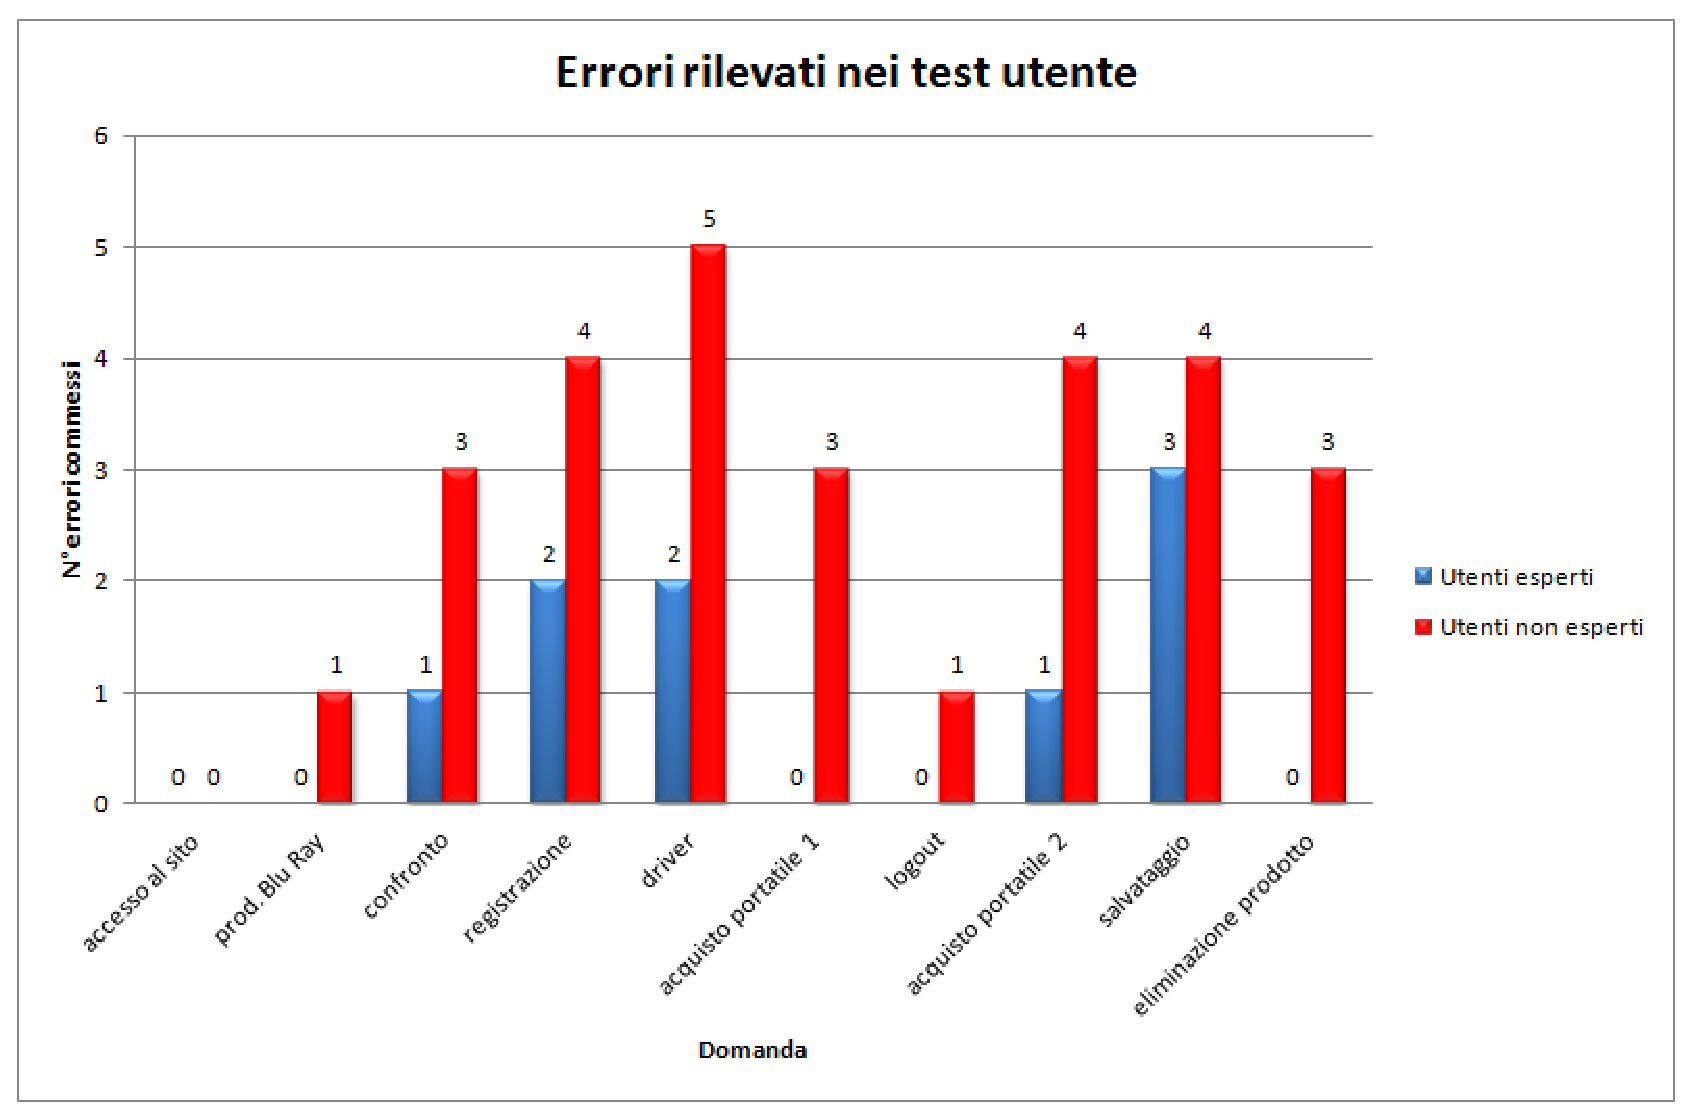
\includegraphics[angle=90, scale=0.75]{figure/grafico_errori_test_utente.eps}
\caption{rafico riportante il numero di errori commessi dagli utenti nella risoluzione dei vari task}
\label{fig:errori_test}
\end{figure}

Dal primo grafico(figura: \ref{fig:tempi_esecuzione_test}) si evince che i tempi impiegati dagli utenti non esperti siano spesso inaccettabili: la ricerca di drivers e software per il computer, cos� come la registrazione hanno comportato lo sforamento del tempo massimo. \\ 
In particolare la registrazione � stata particolarmente ostica per gli utenti non esperti, dovuta a pi� problemi sovrapposti: in primo luogo  non � immediatamente visibile alcun bottone di registrazione, portando l'utente a perdersi all'interno del sito alla ricerca di un link che mandi alla registrazione. Dopo ci� lo scoglio successivo � stata la compilazione dei vari form: ha spesso costretto a ricompilare pi� volte i campi errati, resettando i campi della password ogni iterazione, cosicch� gli utenti che avevano gi� commesso un errore (o pi� errori) hanno avuto un ulteriore rischio di sbagliare nei casi in cui la password fosse stata giusta. Infine le diciture d'errore in lingua inglese non hanno aiutato in alcun modo gli utenti che non parlano questa lingua.\\
Altra operazione che comporta notevole spreco di tempo � la configurazione dei computer da acquistare: la pagina degli acquisti per privati � piuttosto caotica, non � immediato capire che alcuni passi del wizard possono essere saltati e l'utente � portato a seguire sempre il wizard in maniera lineare; spesso anche gli utenti esperti non si sono resi conto del fatto che fossero presenti scorciatoie.\\
Talvolta anche compiti come la rimorzione di elementi dal carrello si � rivelata pi� lenta del previsto: gli utenti meno esperti hanno spesso perso tempo per cercare di cancellare il portatile dal carrello, uno ha addirittura effettuato il log-out.\\
Pi� in generale va sottolineato che gli strumenti offerti dal sito spesso sono di poco aiuto, caso eclatante � il form per la ricerca libera, il quale avrebbe dovuto velocizzare diversi task, soprattutto per i pi� esperti, purtroppo spesso i risultati delle ricerche avevano poco o nulla a che vedere con quanto desiderato dagli utenti. Un'utente esperto per ovviare al problema ha utilizzato il motore di ricerca google per effetturare ricerche all'interno del sito Dell, funzionando dove il search engine di Dell aveva fallito.
Gli help e le sezioni di aiuto non sono mai state usate da nessun utente, nemmeno dai meno esperti quando letteralmente si ``perdevano'' all'interno del sito Dell. Ci� sta ad indicare che essi hanno poca visibilit� all'interno della pagina, oppure non sono dove ci si aspetterebbe.\\
Si nota infine che gli utenti meno esperti oltre ad impiegare pi� tempo dei loro colleghi pi� abituati a navigare facciano anche pi� errori, e in alcuni casi hanno pensato di aver concluso il compito senza invece averlo portato a termine (caso del punto 9, dove era richiesto il salvataggio della configurazione).


\cleardoublepage
\chapter{Mock-up}
A seguito dei problemi di usabilità evidenziati nei capitoli precedenti, siamo passati alla fase di stesura di possibili soluzioni. L'elaborazione di modelli, grafici che mirano a risolvere i problemi riscontrati, o che quantomeno ne riducano drasticamente la criticità, prendono il nome di mock-up.\\
\'E da sottolineare come i mock-up siano un'astrazione e spesso siano un compromesso atto a  migliorare l'usabilità del sito web in esame; la scelta di tale compromesso è influenzata dalle conoscenze del gruppo e dalle rispettive esperienze pregresse.\\
Prima di intervenire abbiamo stabilito l'approccio col quale affrontare i problemi:
\begin{itemize}
\item Singolarmente: ha il vantaggio di trattare modularmente ogni problema e ridurre cos il rischio di generare nuovi problemi, durante la risoluzione. Lo svantaggio maggiore  rappresentato dal fatto che con questo metodo si rischia di generare ridondanza e di creare confusione per l'utente.
\item Per gruppi o collezioni:  l'opposto del caso precedente. Si riduce la ridondanza, mirando a ottenere una visone più ampia dei problemi per trovare  soluzioni che possano andare bene per pi problemi contemporaneamente. In questo modo invece aumenta il rischio di generare nuovi problemi.
\end{itemize}
Nel nostro caso  stata scelta la seconda tecnica, in quanto trattandosi spesso di gruppi di pagine, era preferibile avere una visione d'insieme e trattare errori trasversali a pi pagine, piuttosto che concentrarsi su errori di visibilit limitata.\\
C'è anche un altro aspetto da mettere in evidenza, che spesso viene trascurato: il mock-up, inteso come strumento di presentazione solamente grafico, pertanto si potranno avere solo degli screenshot di quello che potrebbe essere il risultato, nel caso la modifica riguardi il layout della pagina, ma come si è spesso notato, alcuni degli errori più gravi, riguardano l'aspetto implementativo; su tali errori si può solamente ragionare a livello teorico, ma l'implementazione di una soluzione non è fattibile in quanto mancano gli strumenti necessari alla realizzazione.\\ 
Verrà poi ricordato che nelle varie sottosezioni, spesso vengono proposte soluzioni, che andrebbero replicate su molte pagine del sistema. In genere si tratta di link dai nomi non chiari, o la mancanza di collegamenti che, se inseriti nel posto corretto, migliorerebbero l'usabilità.\\
\newline
Per poter iniziare la concettualizzazione dei mock-up è stato necessario lavorare in due fasi:
\begin{itemize}
\item Durante la prima fase abbiamo lavorato direttamente sul codice HTML e sui fogli di stile, i cosiddetti CSS. Per modificarli abbiamo impiegato FireBug, un debugger JavaScript, che, tra le altre cose, permette di modificare "a caldo" il codice interpretato dal browser, vedendo immediatamente risultati delle modifiche. Inoltre l'uso di FireBug ci ha permesso di inserire nuovi link e nuovo testo, col medesimo stile del sito Dell. Più nel dettaglio i font utilizzati, i colori di sfondo e altri aspetti legati ai CSS sono rimasti invariati, avendo un riscontro immediato della pagina mostrata all'utente.
\item Durante la seconda fase invece abbiamo impiegato programmi di grafica (Gimp, Paint, Photoshop), utilizzandoli per i ritocchi più pesanti apportati alle pagine. Sono stati utilizzati prevalentemente, quando la modifica del codice avrebbe richesto troppo tempo. Ad esempio per posizionare immagini e blocchi di testo in determinate posizioni all'interno della pagina, o creare riquadri con gli angoli smussati, che in HTML avrebbero richiesto uno sforzo eccessivo. in tal modo, tramite ``taglia e incolla'' abbiamo potuto disporre rapidamente gli elementi nella maniera che si è ritenuta più oppurtuna
\end{itemize}
\section{Mock-up home page sezione casa}
Prima di procedere con la presentazione dei mock-up ideati per questa sezione vi � un concetto che � bene ricordare: alcuni dei cambiamenti illustrati in questa sezione andrebbero riportati su tutte le pagine del sito web, poich� il problema di usabilit� evidenziato � talvolta presente su tutte le pagine del sito web, in questi casi verr� esplicitamente .\\
\begin{figure}[!h]
\centering
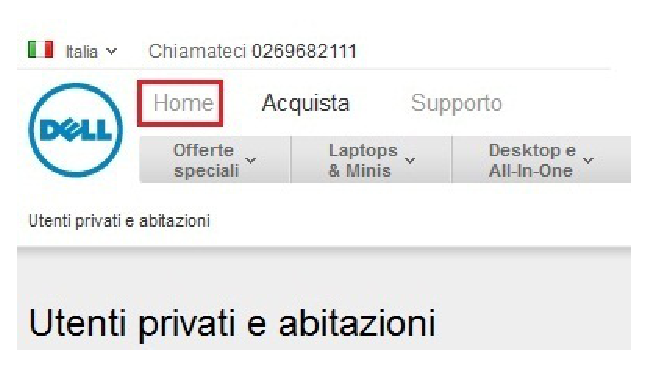
\includegraphics[scale=0.8]{figure/mock_up_home_page.eps}
\caption{Evidenziato in rosso il nuovo link all'Home page. Questo mock-up si applica a tutte le pagine del sito.}
\label{fig:mock_up_non_loggato}
\end{figure}
\begin{figure}[!h]
\centering
\includegraphics[scale=0.8]{figure/mock_up_home_page2.eps}
\caption{Evidenziato in rosso il nuovo link all'Home page. Questo mock-up si applica a tutte le pagine del sito.}
\label{fig:mock_up_non_loggato2}
\end{figure}
\begin{figure}[!h]
\centering
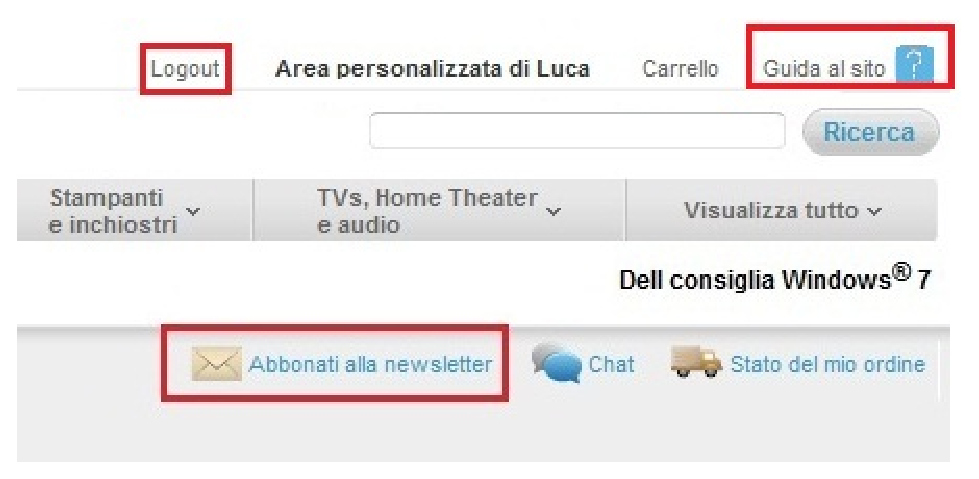
\includegraphics[scale=0.8]{figure/mock_up_home_page_loggato.eps}
\caption{Evidenziate in rosso le modifiche apportate alla home page quando l'utente � loggato.}
\label{fig:mock_up_loggato}
\end{figure}
{\bf Descrizione:} non � immediatamente visibile un link per il ritorno all'home page, non c'� un link diretto che permetta a un nuovo utente di registrarsi e infine il link che punta alla guida al sito � posto in fondo alla pagina, nascosto tra altri link e senza essere posto in evidenza in alcun modo. Il link ``Registrazione e-mail'' non fornisce sufficienti informazioni sull'effetto di tale registrazione.\\
{\bf Proposta di soluzione:} le soluzioni introdotte sono mostrate nelle figure \ref{fig:mock_up_non_loggato} e \ref{fig:mock_up_non_loggato2}. Pi� nel dettaglio abbiamo aggiunto un link ``Home'' sotto al logo Dell, che punta all'home page. La idea di metterlo sotto � stata concepita per separarlo spazialmente dai due link che portano alla sezione per gli acquisti e per il supporto, per marcare ulteriormente questa differenza � stato inoltre impiegato il medesimo colore del logo Dell.\\
A destra del logo sono posizionati due link: ``Registrati'' e ``Guida al sito'', i quali sono stati incorniciati in due linguette, ispirandoci all'idea delle cosiddette tab utilizzate nei moderni web browser (in Firefox e in Chrome, per citarne alcuni). Ci� serve a dare un'idea intuitiva che ci siano due sezioni separate, ma immediatamente accessibili tramite queste linguette. Per completare il mock-up che fa riferimente alla pagina visualizzata quando l'utente non � ancora loggato (figura: \ref{fig:mock_up_non_loggato2}) abbiamo anche pensato di modificare la dicitura ``Sign In'' con ``Accedi''. Nella parte sottostante il link ``Registrazione e-mail'' � stato sostituito con ``Abbonati alla newsletter'', con l'intento di fugare ogni dubbio riguardo allo scopo della sottoscrizione.\\
Per quanto riguarda i link che fanno riferimento alla pagina personale e al logout, abbiamo pensato di rimuovere la parte tra parentesi della dicitura ``Area personalizzata di Luca (L'utente corrente non � Luca?)'', ritenuta ridondante, e affiancarla da un opportuno link di logout.\\
\newline
In questa sezione abbiamo deciso d'inserire anche il mock-up del form di login, modificato come in figura \ref{fig:form_login}.\\
{\bf Descrizione:} Il form del login � di per s� molto semplice e non ha avuto bisogno di un restyling degno di nota. Ci� che rappresenta il problema fondamentale, � il corretto funzionamento del sistema a fronte di due casi:
\begin{itemize}
\item Se si chiude la finestra di login durante la visualizzazione della progress bar, e successivamente si richiede un nuovo login il sitema � ancora in attesa della verifica dei dati inseriti precedentemente. A questo punto viene mostrata una pagina che riporta "caricamento in corso", tuttavia lo stato del sistema non cambia fintanto che l'utente non carica un'altra pagina o non effettua il refresh della pagina corrente.
\item Dopo sei tentativi errati d'inserimento delle credenziali il sistema dovrebbe procedere alla disattivazione dell'account. Tuttavia inserendo le credenziali corrette, anche dopo sei tentativi errati l'account continua a funzionare.
\end{itemize} 
{\bf Proposta di soluzione:} come accennato in precedenza l'aspetto grafico della finestra non necessita di grossi cambiamenti, e l'unico ad essere introdotto � una label che spiega il significato degli asterischi.\\ 
Diverso � l'intervento implementabile:
\begin{itemize}
\item Durante la fase di autenticazione, mentre � mostrata la progress bar, se la finestra viene chiusa, il sistema dovrebbe cercare di ritornare allo stato precedente a quello dell'inserimento dei dati, nel caso il browser non reindirizzasse l'utente � invtato a cliccare su un apposito link (descrizione e mock-up pi� avanti AAAAAAAAAAAAAAAAAAAAAAAAAAAAAAAAAAAAAAAAAAAAAAAAAAAAAAAAAAA\\AAAAAAAAAAAAAAAAAAAAAAAAAAAAAAAAAAAAAAAAAAAAAAAAAAAAA sarebbe meglio dare un riferimento). 
\item Per quanto riguarda la disattivazine dell'account abbiamo invece pensato che che sarebbe pi� opportuno disattivare temporaneamente la possibilit� di login dall'indirizzo ip dal quale sono provenuti i tentativi di login falliti. Questo per prevenire che utenti malintenzionati falliscano intenzionalmente il login per bloccare l'account. Il nostro approccio limiterebbe comunque la portata di attacchi di tipo brute-force.\\ 
\end{itemize}
\begin{figure}[!h]
\centering
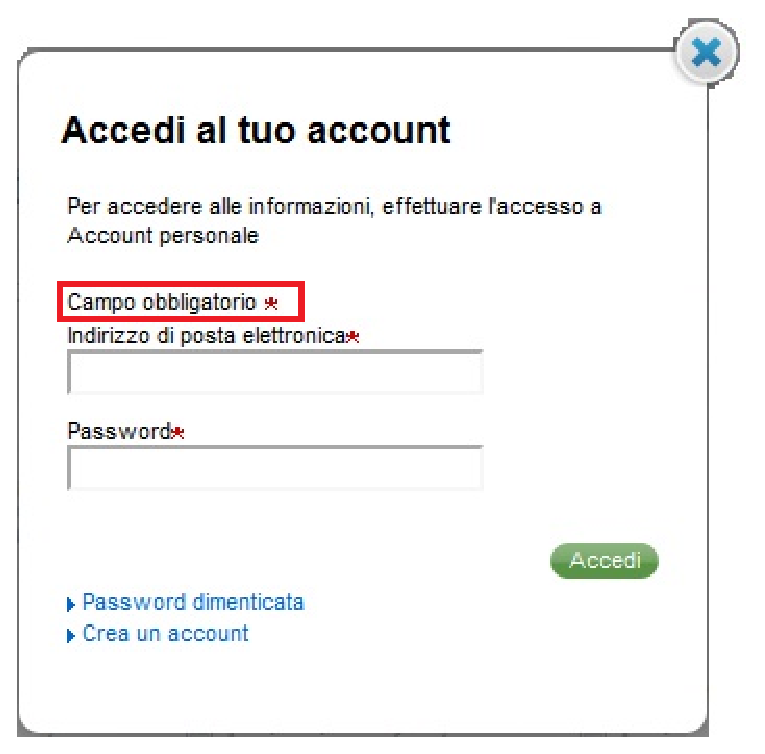
\includegraphics[scale=0.65]{figure/mock_up_fom_login.eps}
\caption{Evidenziate in rosso le modifiche apportate alla home page quando l'utente � loggato}
\label{fig:form_login}
\end{figure}

{\bf Descrizione}: all'interno della pagina relativa ai dati personali dell'utente non esiste un link che rimandi alla pagina in cui l'utente pu� cancellare il proprio account. Ci� pu� essere vincolante poich�, a nostro avviso, un utente dovrebbe avere la libert� di potersi ritirare la propria iscrizione in ogni momento.
{\bf Proposta di soluzione}: all'interno della pagina contenente i dati personali viene aggiunta una voce al men� di sinistra chiamata ``cancellazione account''. In tal modo si pu� accedere a una sezione, che verr� aperta sulla destra rispetto al men�, in cui l'utente potr� cancellare il proprio account. Dal punto di vista implementativo, si � pensato che fosse opportuno far comparire un popup che chieda l'inserimento della password dell'utente per confermare la cancellazione,come vincolo di sicurezza contro cancellazioni accidentali.(figura \ref{fig:mockup_cancellazione_account}).

\begin{figure}[!h]
\centering
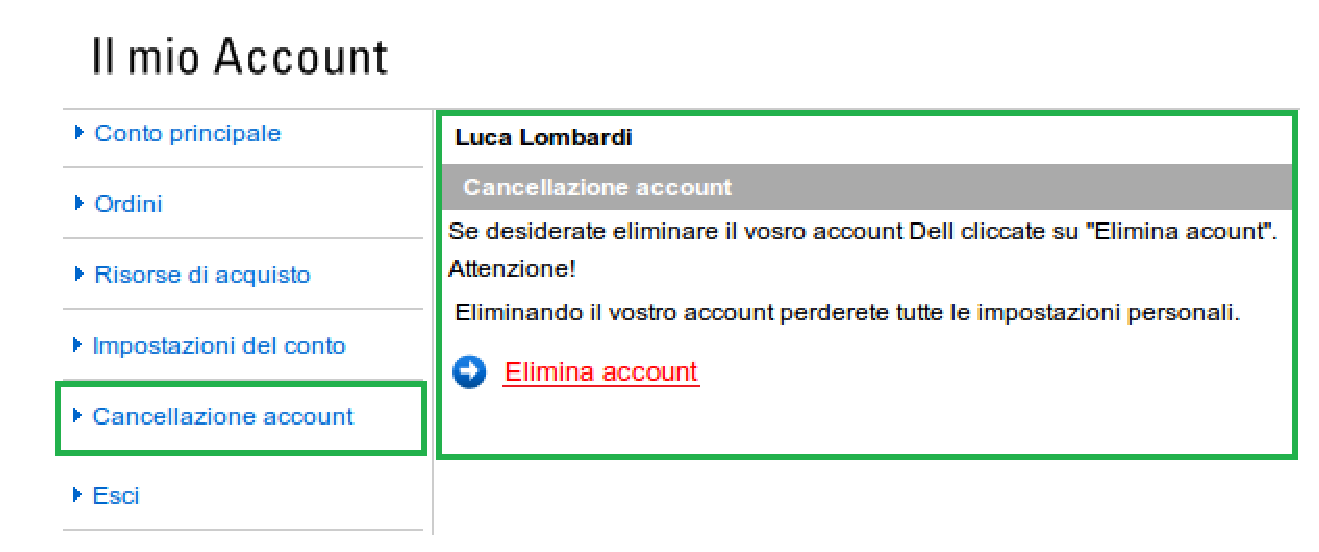
\includegraphics[scale=0.7]{figure/mock_up_cancellazione.eps}
\caption{In verde sono evidenziate le parti aggiunte che consentono all'utente di cancellare il proprio account.}
\label{fig:mockup_cancellazione_account}
\end{figure}

{\bf Descrizione}: come anticipato nella sezione dedicata ai problemi di usabilit�, se l'utente chiude la finestra di dialogo, nel momento in cui il sistema sta verificando le credenziali, il sitema rimane in uno stato ibrido in cui l'utente non pu� effettuare un nuovo login e il sistema non riconosce ancora l'utente.\\
{\bf Proposte di soluzione}: per ovviare a tale problema abbiamo pensato di introdurre una redirezione automatica dalla pagina che compare alla chiusura della finestra di dialogo, nel caso in cui il browser fallisse la redirezione diamo all'utente la possibilit� di forzare il sistema ad uscire dallo stato nel quale � caduto. Mock-up mostrato in figura \ref{fig:mock_up_login_reindirizzo}. \\

\begin{figure}[!h]
\centering
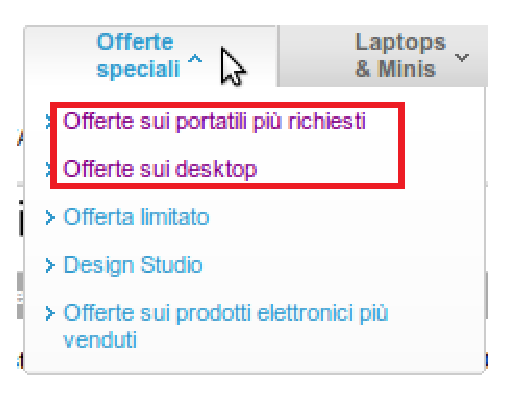
\includegraphics[scale=0.6]{figure/mock_up_link_usati.eps}
\caption{Riquadrati in rosso la modfica del colo dei link gi� selezionati dall'utente}
\label{fig:mock_up_link_usati}
\end{figure}

{\bf Descrizione}: come segnalato in precedenza, il sistema spesso non offre all'utente un riscontro sui link gi� usati (per esempio nei menu a tendina in cima alla pagina), all'interno di una stessa sessione di lavoro.\\
{\bf Proposte di soluzione}: come riportato in figura \ref{fig:mock_up_link_usati} si pu� notare come i link selezionati almeno una volta siano colorati in modo diverso, dando all'utente un aiuto qualora cerchi una pagina visitata in precedenza e l'operatore di BACK del browser non gli possa essere d'aiuto.

\begin{figure}[!h]
\centering
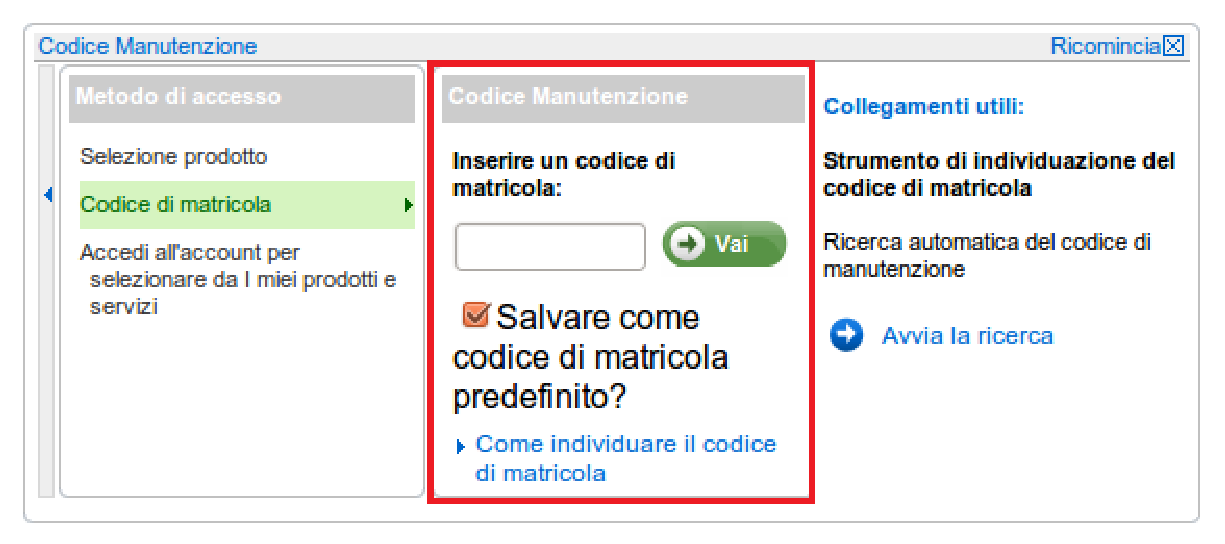
\includegraphics[scale=0.75]{figure/mock_up_manutenzione.eps}
\caption{il men� viene espanso leggermente per evitare la scroll bar, come invece era fatto nella versione originale (figura:\ref{fig:manutenzione})}
\label{fig:mock_up_manutenzione}
\end{figure}

{\bf Descrizione}: dalla figura \ref{fig:manutenzione} si pu� vedere che l'area dedicata al ``Codice di matricola'', � estramente ridotta e si deve ricorrere a una scroll bar per consentire all'utente di visualizzare tutto il contenuto: abbiamo in questo caso un help nascosto, ci� risulta estremamente scomodo, considerato che nella pagina � presente molto spazio inutilizzato.\\
{\bf Proposte di soluzioni}: viene ampliata l'intera area, fino a che la scroll bar non scompare, in tal modo l'utente pu� accedere a tutte le informazioni in modo diretto.


\begin{figure}[!h]
\centering
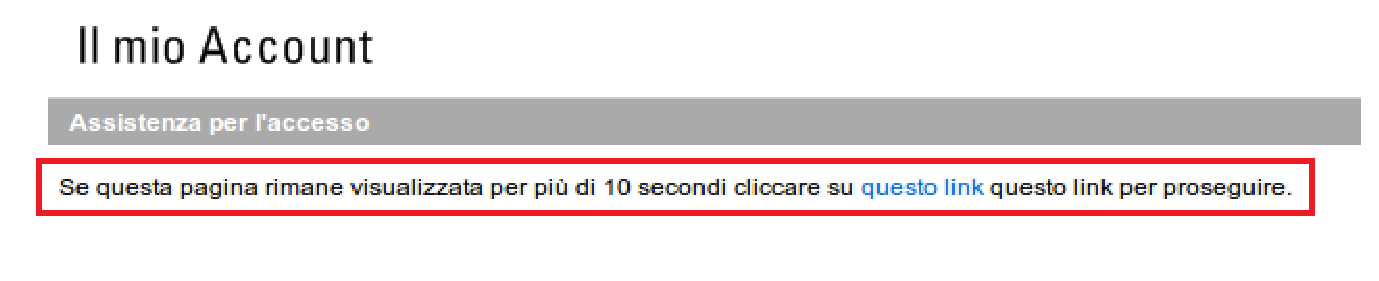
\includegraphics[scale=0.6]{figure/mock_up_login_reindirizzo.eps}
\caption{Nel caso il form del login non reindirizzi automaticamente, viene data la possibilit� all'utente di agire manualmente}
\label{fig:mock_up_login_reindirizzo}
\end{figure}
{\bf Descrizione}: nella figura \ref{fig:mock_up_riepilogo} sono evidenziate le modifiche apportate alla pagina di configurazione del propriro sistema Dell. Come anticipato nella sezione relativa ai problemi di usabilit�, la pagina relativa alla scelta per la copertura sui danni accidentali, non ha alcun riferimento alle condizioni contrattuali, ma solo vaghe spiegazioni dal carattere pubblicitario. Inoltre la finestra di riepilogo delle componenti scelte per la personalizzazione � molto ristretta, costringendo l'utente a un continuo uso dello scroll per scorrere tale riassunto.\\
{\bf Proposta di soluzione}: viene aggiunto un link alla documentazione per gli esatti termini contrattuali dell'estensione di garanzia proposta. Inoltre la finestra di riepilogo dei componenti selezionati dall'utente, posta nella parte destra della pagina, viene espansa in modo da mostrare pi� componenti contemporaneamente.
\begin{figure}[!h]
\centering
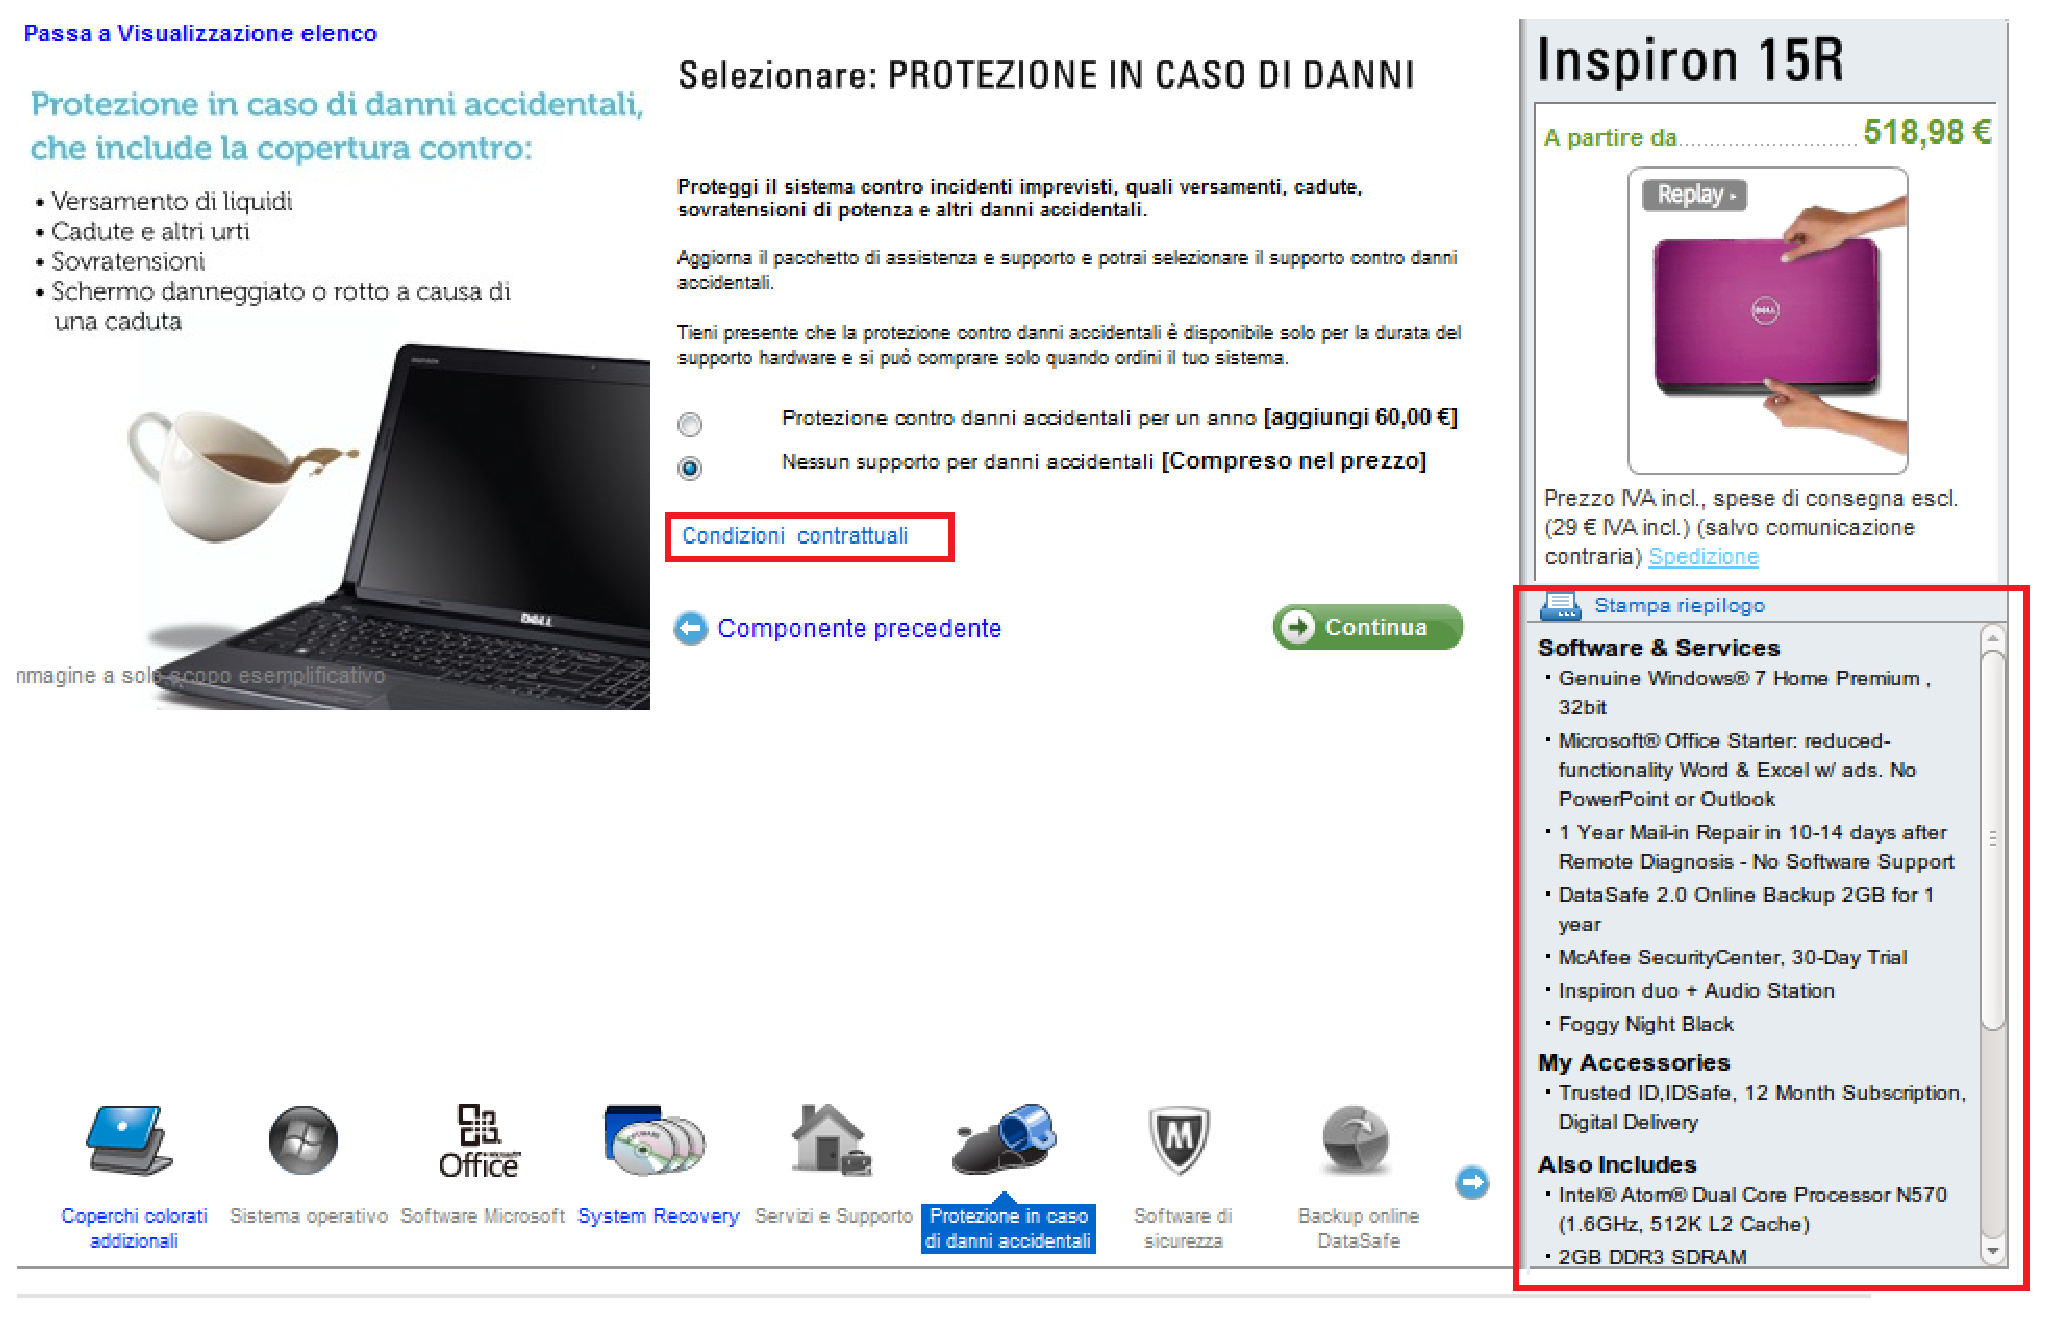
\includegraphics[scale=0.7,angle=90]{figure/mock_up_riepilogo.eps}
\caption{Mock-up sulla pagina di configurazione del computer}
\label{fig:mock_up_riepilogo}
\end{figure}
\newline
{\bf Descrizione}: come anticipato nella sezione relativa ai problemi di usabilit�, un problema di un certo rilievo � il sovraffollamento delle due sezioni ``Acquista'' e ``Supporto'', che rendono difficoltosa la navigazione. 
Di seguito analizzeremo le due soluzioni proposte, motivando le scelte effettuate.
\begin{itemize}
\item {\bf Sezione Acquisti}: innanzitutto � stata analizzata la home page della sezione degli acquisti. Come si pu� notare dalle figura mostrata nella sezione relativa ai problemi di usabilit�, in figura \ref{fig:schermata_incasinata}, la pagina mostrata all'utente � troppo densa densa di informazioni, i titoli delle macrosezioni non sono cliccabili, sono presenti link duplicati che puntano alle medesime sezioni e al tutto sono mescolati banner pubblicitari. Sicuramente � utile usare banner pubblicitari per mettere in risalto alcuni prodotti, siccome il sito ha anche lo scopo di essere una vetrina d'esposizione per i propri prodotti, tuttavia la loro collocazione spaziale inficia la navigabilit�.\\

{\bf Proposte di soluzione}: per ovviare a tali problemi si � pensato a una totale riorganizzazione e razionalizzazione dei contenuti, senza la contempo precludere la possibilit� di aggiungere della pubblicit�. \\
Nella figura \ref{fig:mockup_sez_acquisti_pagina_intera} si pu� vedere come si � pensato di riorganizzare il tutto:
\begin{itemize}
Di seguito elenchiamo i cambiamenti introdotti dal mock-up:
\item Innanzitutto spariscono tutte le immagini pubblicitarie che, eventualmente, potranno essere poste ai lati del corpo centrale della pagina.
\item Delle sei sezioni presenti in precedenza (vedere figura:\ref{fig:schermata_incasinata}) ne manteniamo solo quattro, scelte in modo tale che racchiudano tutti i prodotti: ``Notebook \& Mini'', ``Desktop e All-in-One'', ``Monitor'', ``Elettronica e Accessori''. Tramite esse si accede alle varie sottosezioni. Si � ritenuto utile porre al di sotto di ogni immagine alcuni link, come acceleratori per accedere direttamente alle pagine relative alle principali sotto-categorie. In ogni caso abbiamo cercato di fare si che tali link non costituiscono la parte preponderante della pagina e non siano d'intralcio durante la navigazione.
\item Al di sotto di questa sezione vengono proposte due sezioni in chiara evidenza, nel caso l'utente necessitasse di assistenta per l'acquisto di un prodotto. Le due aree scelte sono dedicate all'assistenza tramite chat, oppure assistenza telefonica. L'assistenza tramite chat rimanda all'apposita sezione, all'assistenza telefonica invece non ne � dedicata nessuna, riportando solo il numero di telefono.  
\end{itemize}

\begin{figure}[!h]
\centering
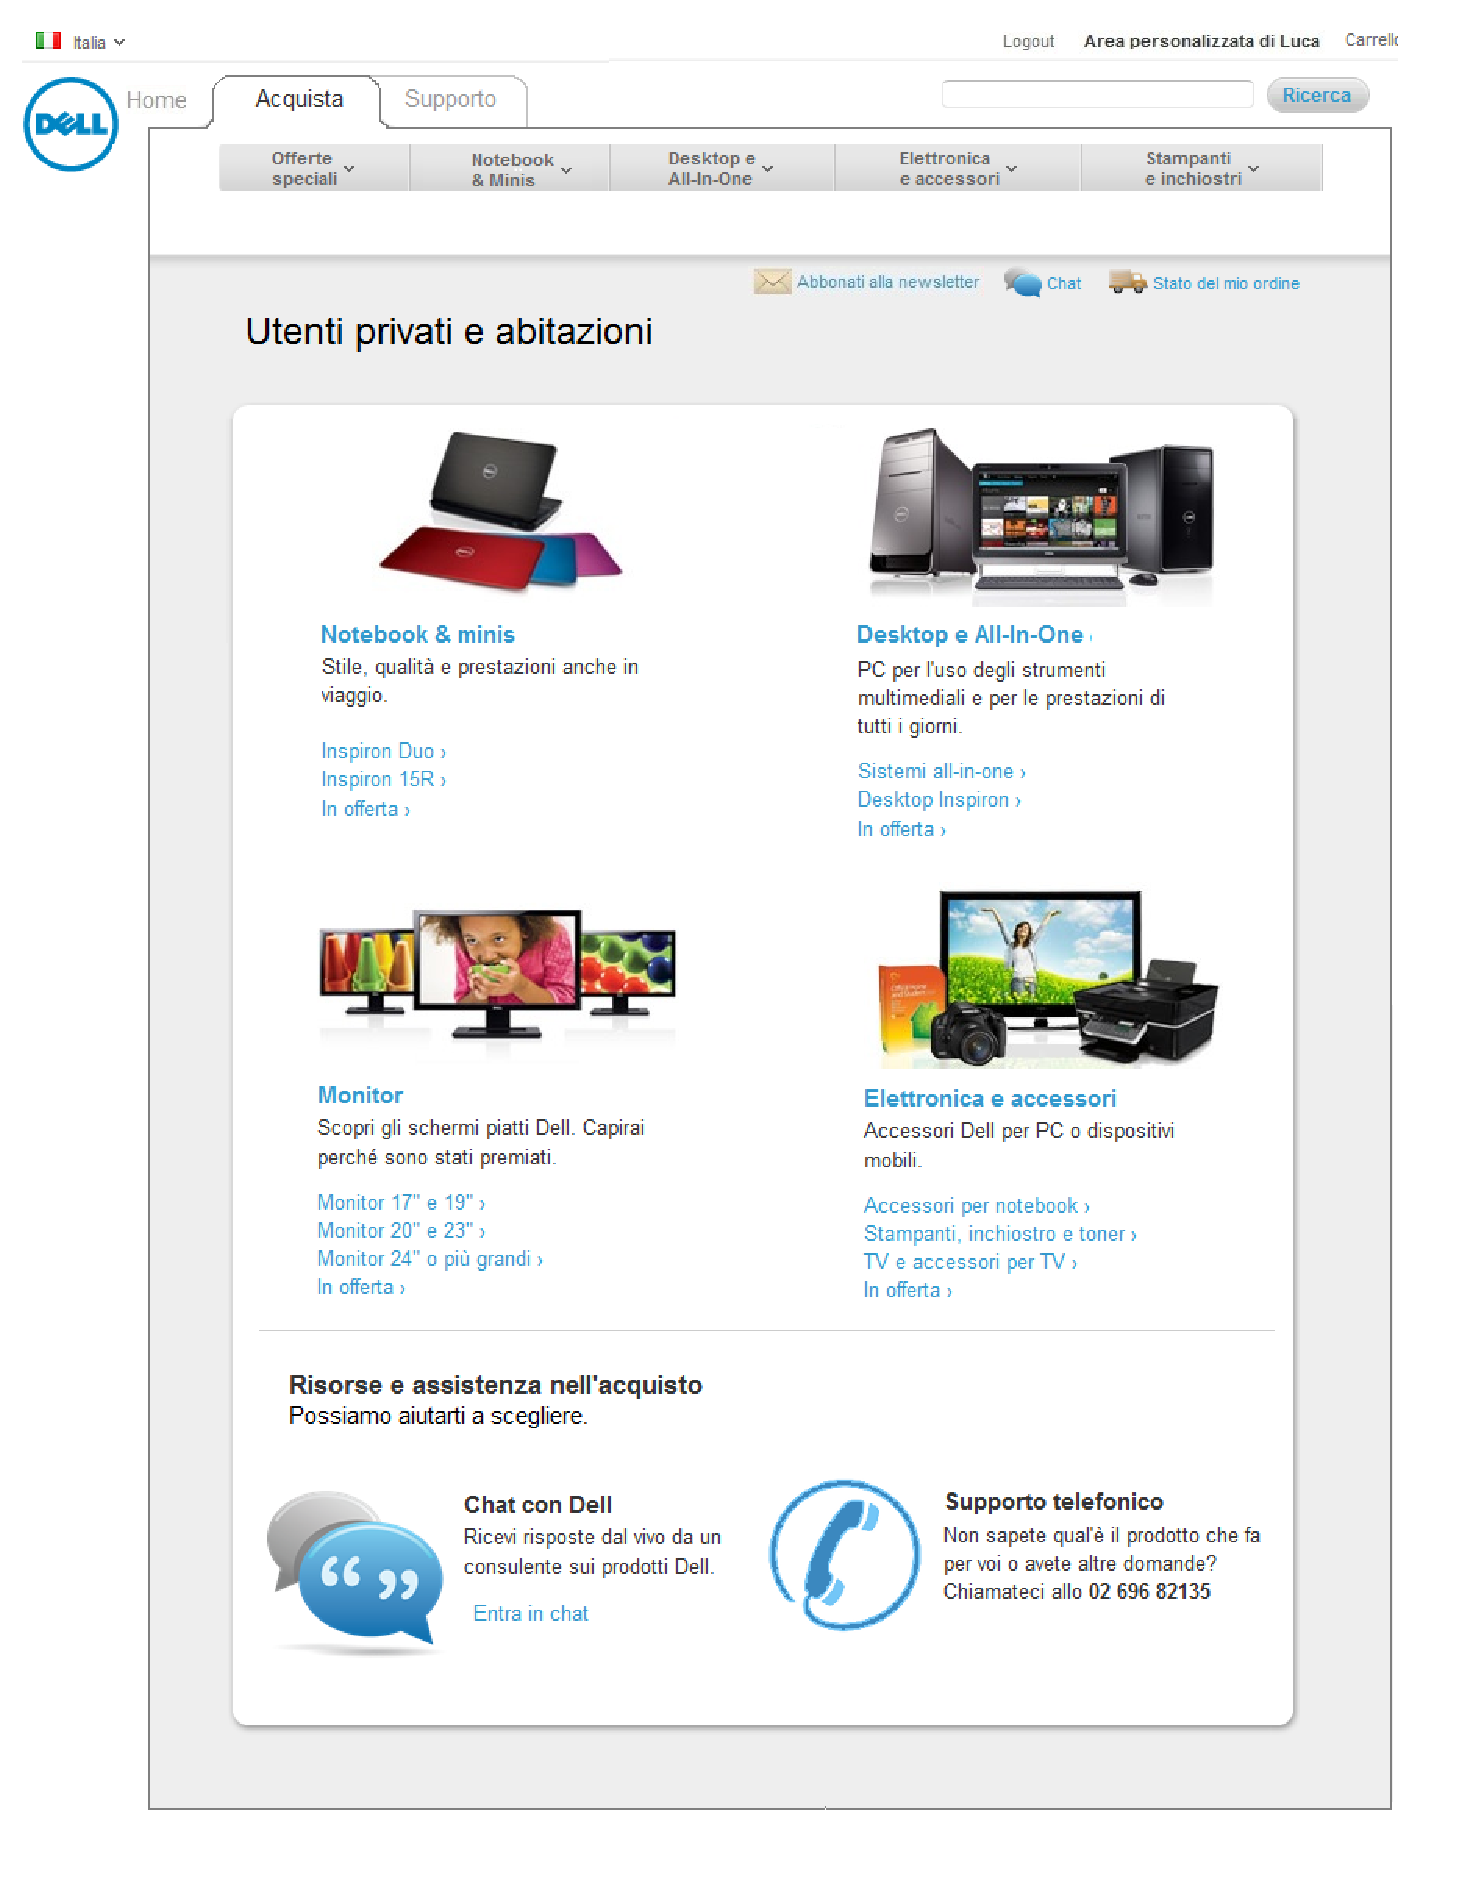
\includegraphics[scale=0.52]{figure/mockup_sez_acquisti_pagina_intera.eps}
\caption{Mock-up della sezione acquisti}
\label{fig:mockup_sez_acquisti_pagina_intera}
\end{figure}

\item{\bf Descrizione}: la sezione di supporto, soffre anch'essa di sovraffollamento di link, spesso ripetuti, che disorientano l'utente meno esperto. In questa sezione non ci sono banner pubblicitari, ma la pagine risultano essere dense di link e testo. Sotto le immagini spesso vengono proposte lunghe liste di link, che rallentano la ricerca dei contenuti desiderati.
{\bf Proposte di soluzione}: per migliorare la pagina sono state introdotte radicali modifiche al layout:
\begin{itemize}
\item I quattro gruppi principali di icone poste a centro pagina, sono stati unite ai sei che si trovano poco pi� sotto, all'interno della parte ``Altri strumenti di supporto''. In tal modo si sono ottenuti sette macro sezioni, che racchiudono e suddividono in categorie le tipologie di problemi che potrebbe avere l'utente. Tali categorie sono:
\begin{itemize}
\item Driver e Hardware: sezione dedicata ai driver, aggiornamenti e richiesta di assistenza per  l'hardware del computer. Da tale sezione di pu� accedere alla sezione di download di aggiornamenti per firmware e altro software strttamente legato al funzionamento dei componenti fisici del computer.
\item Guide e Tutorial: sezione dedicata alla documentazione per poter consentire all'utente di consultare manuali e trovare risposte alla domande pi� frequenti.
\item Supporto per Windows: sezione che riguarda tutti i sistemi Microsoft che sono venduti sulle macchine Dell. All'interno si accede a una pagina che permette all'utente di scegliere fra i vari sistemi operativi, trovare risposte che riguardano il buon funzionamento del sistema operativo.
\item Stato dell'ordine e supporto: sezione rivolta a chi necessita di avere risposte e assistenza per effettuare correttamente un ordine, avere notizie riguardate lo stato si un ordine gi� effettuato.
\item Sicurezza e virus: sezione dedicata alla sicurezza del sistema Dell acquistato.
\item Connettivit� e reti: sezione dedicata alla configurazione e gestione di una rete domestica, sia calbata che wireless.
\item Stampanti e altre periferiche: sezione dedicata all'installazione e configurazione in una periferica collegata poi a un sistema Dell. In tale sezione si trova anche supporto per le periferiche di marchio Dell.
\end{itemize}
\item Sotto alle sette categorie di cui sopra ne abbiamo poste altre quattro che non accorpabili alle  precedenti, e sono meno importanti delle precedenti:
\begin{itemize}
\item Forum Dell: link dedicato all'accesso alla community per avere assistenza da altri utenti.
\item Informazioni sulla garanzia: link che permette di accedere alla visione del contratto di garanzia che l'utente stipula al momento dell'acquisto di un prodotto Dell.
\item Cronologia e stato di supporto: qualora la richiesta di assistenza non fosse immediatamente soddisfatta, in questa sezione l'utente pu� avere informazioni e aggiornamenti sulla propria domanda di supporto.
\item Strumenti e applicazioni: sezione dedicata a come trovare i vari codici, e diciture dei compoenti hardware e software che sono spesso richiesti dall'assistenza.
\end{itemize}
\item A fianco del corpo centrale, a sinistra � riproposta una colonna di link, che a dispetto della versione precedente (figura: \ref{fig:supporto_senza_modifiche}), ha molti meno link. Nella nuova versione infatti sono stati riportati solamente:
\begin{itemize}
\item un link all'home page della sezione di supporto;
\item una serie di contatti diretti con gli operatori specializzati (vendita, ordine, tecnici).
\item una lista composta da otto link, che riportano le otto domande pi� frequenti poste nell'ultimo periodo. Tale lista � variabile, in quanto le domande poste pi� spesso cambieranno nel tempo, abbiamo ritenuto utile mostrarle come acceleratori.
\end{itemize}
\end{itemize}
\end{itemize}
\begin{figure}[t]
\centering
\includegraphics[scale=0.5]{figure/supporto_senza_modifiche.eps}
\caption{Home page della sezione di supporto prima delle modifiche}
\label{fig:supporto_senza_modifiche}
\end{figure}

\begin{figure}[!h]
\centering
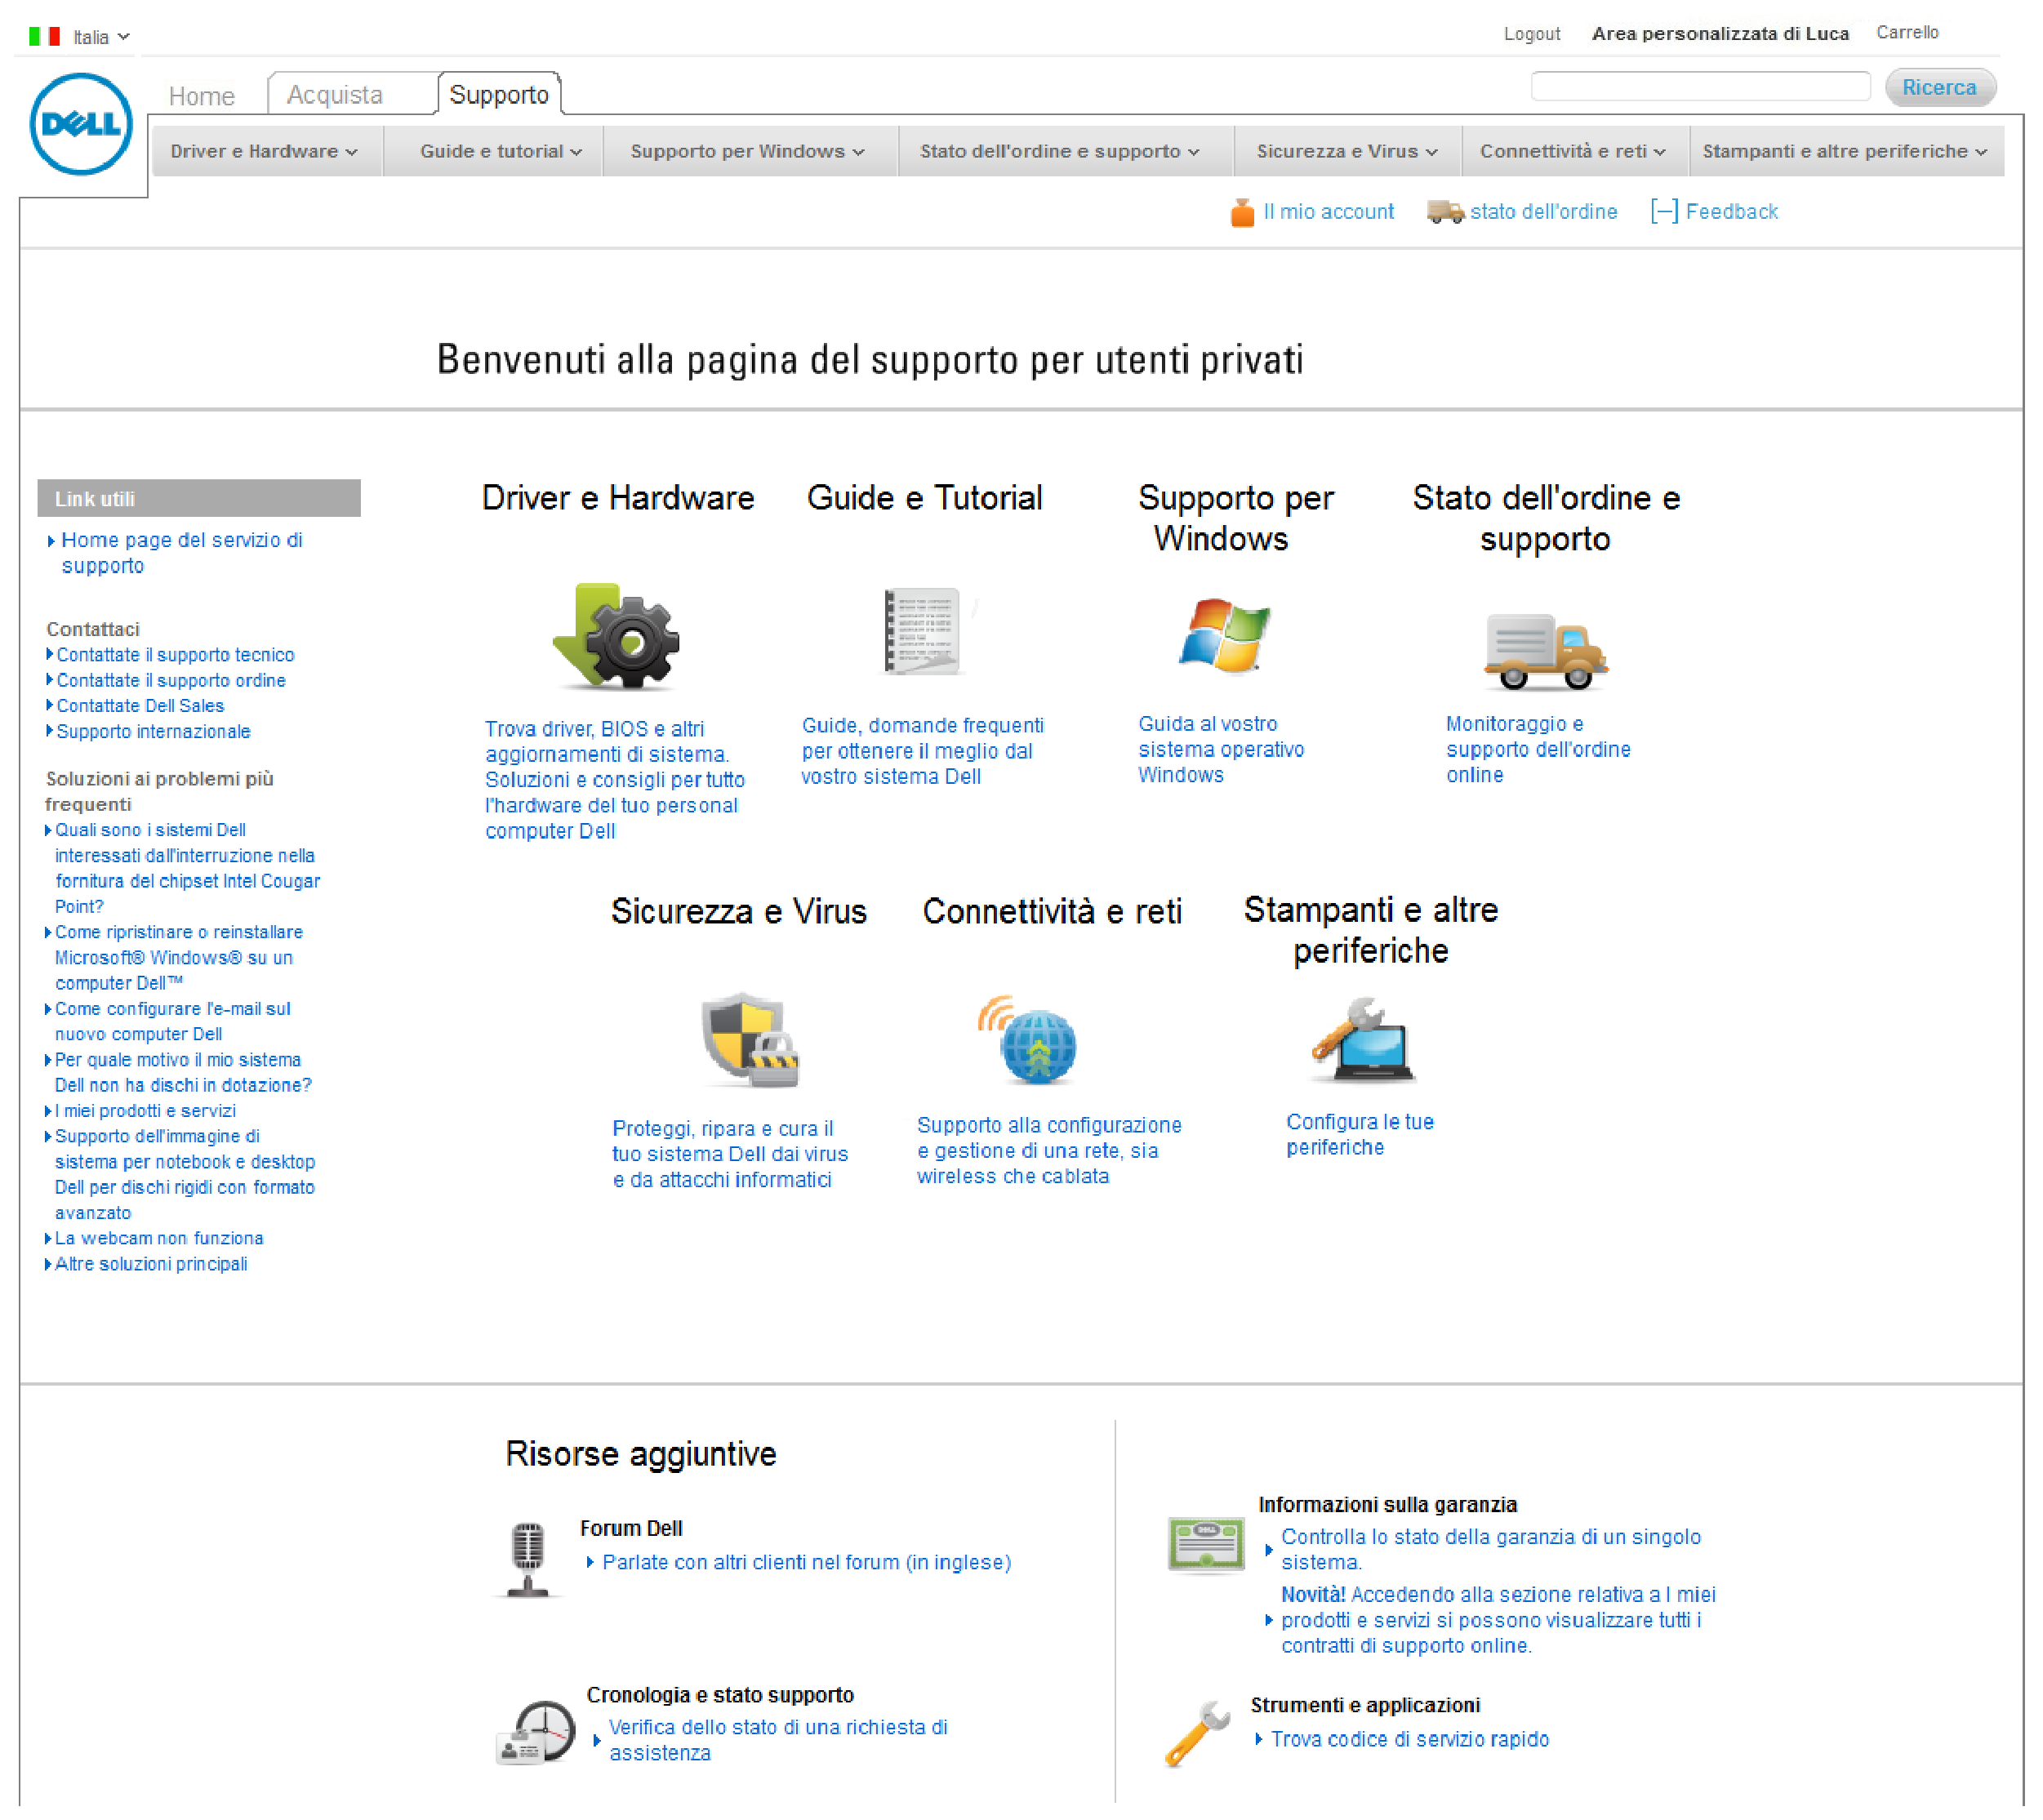
\includegraphics[angle=90,scale=0.45]{figure/mock_up_home_supporto.eps}
\caption{Mock-up della home page della sezione di supporto}
\label{fig:mock_up_home_supporto}
\end{figure}



% ----- appendici  -----

%\appendix

%\cleardoublepage
%\input{appendixA.tex}

%\cleardoublepage
%\input{appendixB.tex}

% ----------------------------

\end{document}
